 
% easychair.tex,v 3.5 2017/03/15

\documentclass{easychair}
%\documentclass[EPiC]{easychair}
%\documentclass[EPiCempty]{easychair}
%\documentclass[debug]{easychair}
%\documentclass[verbose]{easychair}
%\documentclass[notimes]{easychair}
%\documentclass[withtimes]{easychair}
%\documentclass[a4paper]{easychair}
%\documentclass[letterpaper]{easychair}

\usepackage{pifont}
\usepackage{xcolor}
\usepackage{comment}

\definecolor{second}{HTML}{007000}

\usepackage{doc}

\usepackage{cite}

% pretty tables defined with data files
\usepackage{booktabs}
\usepackage{longtable}
\usepackage{pgfplotstable}
\usepackage{titlesec}
\usepackage{multirow}
\usepackage{subcaption}
\usepackage{fancyvrb}
\usepackage{cleveref}

\pgfplotsset{compat=1.16}


% long table macro for pgfplotstable
% see https://tex.stackexchange.com/questions/66504/pgfplotstable-longtable-with-caption-and-repeating-header
\pgfkeysifdefined{/pgfplots/table/output empty row/.@cmd}{
    % upcoming releases offer this more convenient option:
    \pgfplotstableset{
        empty header/.style={
          every head row/.style={output empty row},
        }
    }
}{
    % versions up to and including 1.5.1 need this:
    \pgfplotstableset{
        empty header/.style={
            typeset cell/.append code={%
                \ifnum\pgfplotstablerow=-1 %
                    \pgfkeyssetvalue{/pgfplots/table/@cell content}{}%
                \fi
            }
        }
    }
}
%%%-----------------------------------------------

% use this if you have a long article and want to create an index
% \usepackage{makeidx}

% In order to save space or manage large tables or figures in a
% landcape-like text, you can use the rotating and pdflscape
% packages. Uncomment the desired from the below.
%
% \usepackage{rotating}
% \usepackage{pdflscape}

% Some of our commands for this guide.
%
\newcommand{\easychair}{\textsf{easychair}}
\newcommand{\miktex}{MiK{\TeX}}
\newcommand{\texniccenter}{{\TeX}nicCenter}
\newcommand{\makefile}{\texttt{Makefile}}
\newcommand{\latexeditor}{LEd}

\newcommand{\todoForParticipants}[1]{\textcolor{red}{TODO-PARTICIPANTS: #1}}

\newcommand{\todo}[1]{\textcolor{red}{TODO: #1}}

\titlespacing*{\paragraph}
{0pt}{2pt}{5pt}
%\makeindex

%% Front Matter
%%
% Regular title as in the article class.
%
\title{The Third International Verification of Neural Networks Competition (VNN-COMP 2022): Summary and Results%
%\thanks{Other people who contributed to this document include Maria Voronkov   (Imperial College and EasyChair) and Graham Gough (The University of Manchester).}
}

% Authors are joined by \and. Their affiliations are given by \inst, which indexes
% into the list defined using \institute
%
\author{Stanley Bak\thanks{S. Bak is with Stony Brook University, \tt stanley.bak@stonybrook.edu.}, Changliu Liu\thanks{C. Liu is with Carnegie Mellon University, \tt cliu6@andrew.cmu.edu.}, Taylor Johnson\thanks{T. Johnson is with Vanderbilt University, \tt taylor.johnson@vanderbilt.edu.}
%Serguei A. Mokhov\inst{1}\thanks{Designed and implemented the class style}
%\and
%    Geoff Sutcliffe\inst{2}\thanks{Did numerous tests and provided a lot of suggestions}
%\and
%   Andrei Voronkov\inst{3}\inst{4}\inst{5}\thanks{Masterminded EasyChair and created versions
%     3.0--3.5 of the class style}
}

% Institutes for affiliations are also joined by \and,
\institute{
%  Concordia University,
%  Montreal, Quebec, Canada\\
%  \email{mokhov@cse.concordia.ca}
%\and
%   University of Miami,
%   Miami, Florida, U.S.A.\\
%   \email{geoff@cs.miami.edu}\\
%\and
%   University of Manchester,
%   Manchester, U.K.\\
%   \email{andrei@voronkov.com}\\
%\and
%   Chalmers University of Technology,
%   Gothenburg, Sweden
%\and
%   EasyChair
 }

%  \authorrunning{} has to be set for the shorter version of the authors' names;
% otherwise a warning will be rendered in the running heads. When processed by
% EasyChair, this command is mandatory: a document without \authorrunning
% will be rejected by EasyChair

\authorrunning{}
\date{\phantom{date}\\}
% \titlerunning{} has to be set to either the main title or its shorter
% version for the running heads. When processed by
% EasyChair, this command is mandatory: a document without \titlerunning
% will be rejected by EasyChair
\titlerunning{VNN-COMP 2022 Report}

\begin{document}

\maketitle

\begin{abstract}
This report summarizes the third International Verification of Neural Networks Competition (VNN-COMP 2021), held as a part of the 5th Workshop on Formal Methods for ML-Enabled Autonomous Systems (FOMLAS) that was collocated with the 34th International Conference on Computer-Aided Verification (CAV).
%
%Twelve teams participated in this competition.
%
The goal of the competition is to provide an objective comparison of the state-of-the-art methods in neural network verification, in terms of scalability and speed.
%
Along this line, we used standard formats (ONNX for neural networks and VNNLIB for specifications), standard hardware (all tools are run by the organizers on AWS), and tool parameters provided by the tool authors.
%
This report summarizes the rules, benchmarks, participating tools, results, and lessons learned from this competition.
\end{abstract}



%------------------------------------------------------------------------------
%\input{tables}
\section{Total Score}

%Total Score:

\begin{table}[h]
\begin{center}
\caption{Overall Score} \label{tab:score}
{\setlength{\tabcolsep}{2pt}
\begin{tabular}[h]{@{}lll@{}}
\toprule
\textbf{\# ~} & \textbf{Tool} & \textbf{Score}\\
\midrule
1 & $\alpha$,$\beta$ Crown & 1099.5 \\
2 & Neuralsat & 883.1 \\
3 & Pyrat & 613.6 \\
4 & Nnenum & 442.8 \\
5 & Nnv & 240.4 \\
6 & Fastbatllnn & 100.0 \\
\bottomrule
\end{tabular}
}
\end{center}
\end{table}



\begin{figure}[h]
\centerline{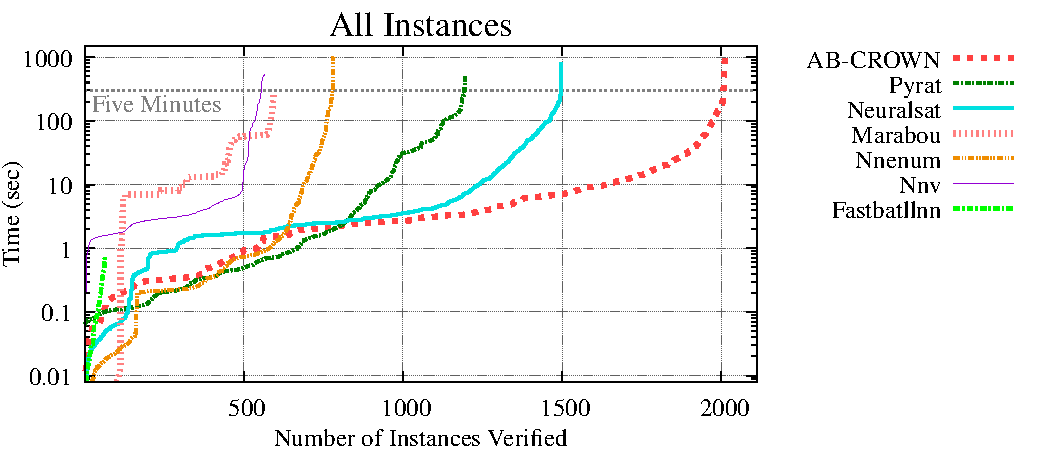
\includegraphics[width=\textwidth]{cactus/all.pdf}}
\caption{Cactus Plot for All Instances.}
\label{fig:quantPic}
\end{figure}





\clearpage
\section{Scored Benchmarks}

% Category 2023_acasxu (single_overhead=True):

\begin{table}[h]
\begin{center}
\caption{Benchmark \texttt{2023-acasxu}} \label{tab:cat_{cat}}
{\setlength{\tabcolsep}{2pt}
\begin{tabular}[h]{@{}llllllrr@{}}
\toprule
\textbf{\# ~} & \textbf{Tool} & \textbf{Verified} & \textbf{Falsified} & \textbf{Fastest} & \textbf{Penalty} & \textbf{Score} & \textbf{Percent}\\
\midrule
1 & nnenum & 139 & 47 & 0 & 0 & 1860 & 100.0\% \\
2 & $\alpha$-$\beta$-CROWN & 139 & 47 & 0 & 0 & 1860 & 100.0\% \\
3 & NeuralSAT & 138 & 46 & 0 & 0 & 1840 & 98.9\% \\
4 & PyRAT & 137 & 45 & 0 & 0 & 1820 & 97.8\% \\
5 & Marabou & 135 & 46 & 0 & 0 & 1810 & 97.3\% \\
6 & NNV & 68 & 27 & 0 & 0 & 950 & 51.1\% \\
\bottomrule
\end{tabular}
}
\end{center}
\end{table}



\begin{figure}[h]
\centerline{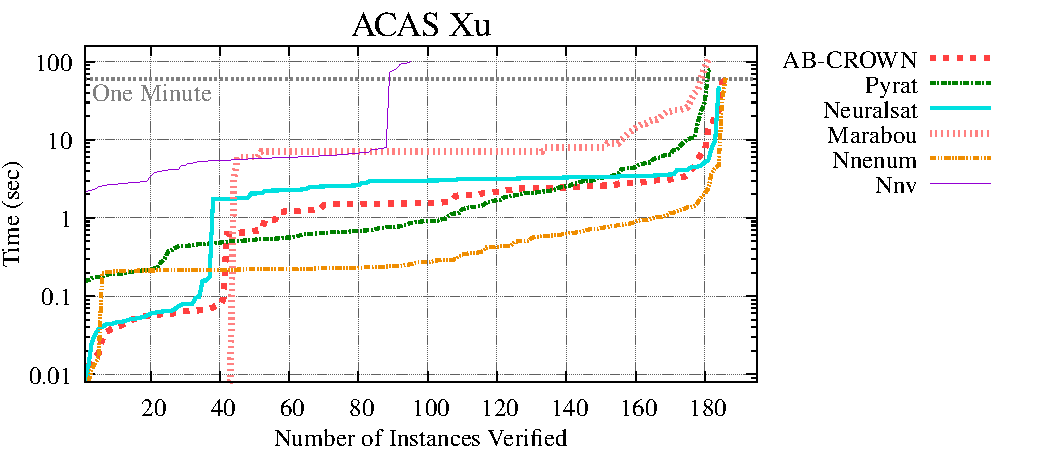
\includegraphics[width=\textwidth]{cactus/2023_acasxu.pdf}}
\caption{Cactus Plot for ACAS Xu.}
\label{fig:quantPic}
\end{figure}


% Category 2023_cgan (single_overhead=True):

\begin{table}[h]
\begin{center}
\caption{Benchmark \texttt{2023-cgan}} \label{tab:cat_{cat}}
{\setlength{\tabcolsep}{2pt}
\begin{tabular}[h]{@{}llllllrr@{}}
\toprule
\textbf{\# ~} & \textbf{Tool} & \textbf{Verified} & \textbf{Falsified} & \textbf{Fastest} & \textbf{Penalty} & \textbf{Score} & \textbf{Percent}\\
\midrule
1 & $\alpha$-$\beta$-CROWN & 8 & 13 & 0 & 0 & 210 & 100.0\% \\
2 & PyRAT & 8 & 11 & 0 & 0 & 190 & 90.5\% \\
3 & nnenum & 6 & 11 & 0 & 0 & 170 & 81.0\% \\
4 & NeuralSAT & 3 & 11 & 0 & 0 & 140 & 66.7\% \\
5 & NNV & 3 & 11 & 0 & 0 & 140 & 66.7\% \\
6 & Marabou & 0 & 13 & 0 & 0 & 130 & 61.9\% \\
\bottomrule
\end{tabular}
}
\end{center}
\end{table}



\begin{figure}[h]
\centerline{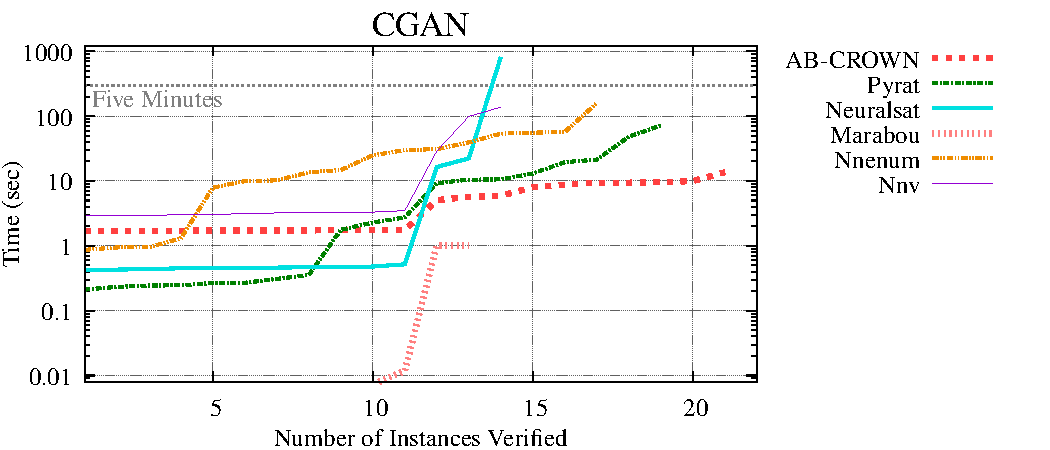
\includegraphics[width=\textwidth]{cactus/2023_cgan.pdf}}
\caption{Cactus Plot for CGAN.}
\label{fig:quantPic}
\end{figure}


% Category 2023_collins_rul_cnn (single_overhead=True):

\begin{table}[h]
\begin{center}
\caption{Benchmark \texttt{2023-collins-rul-cnn}} \label{tab:cat_{cat}}
{\setlength{\tabcolsep}{2pt}
\begin{tabular}[h]{@{}llllllrr@{}}
\toprule
\textbf{\# ~} & \textbf{Tool} & \textbf{Verified} & \textbf{Falsified} & \textbf{Fastest} & \textbf{Penalty} & \textbf{Score} & \textbf{Percent}\\
\midrule
1 & nnenum & 35 & 27 & 0 & 0 & 620 & 100.0\% \\
2 & NeuralSAT & 35 & 27 & 0 & 0 & 620 & 100.0\% \\
3 & Marabou & 35 & 27 & 0 & 0 & 620 & 100.0\% \\
4 & $\alpha$-$\beta$-CROWN & 35 & 27 & 0 & 0 & 620 & 100.0\% \\
5 & PyRAT & 33 & 27 & 0 & 0 & 600 & 96.8\% \\
6 & NNV & 23 & 27 & 0 & 0 & 500 & 80.6\% \\
\bottomrule
\end{tabular}
}
\end{center}
\end{table}



\begin{figure}[h]
\centerline{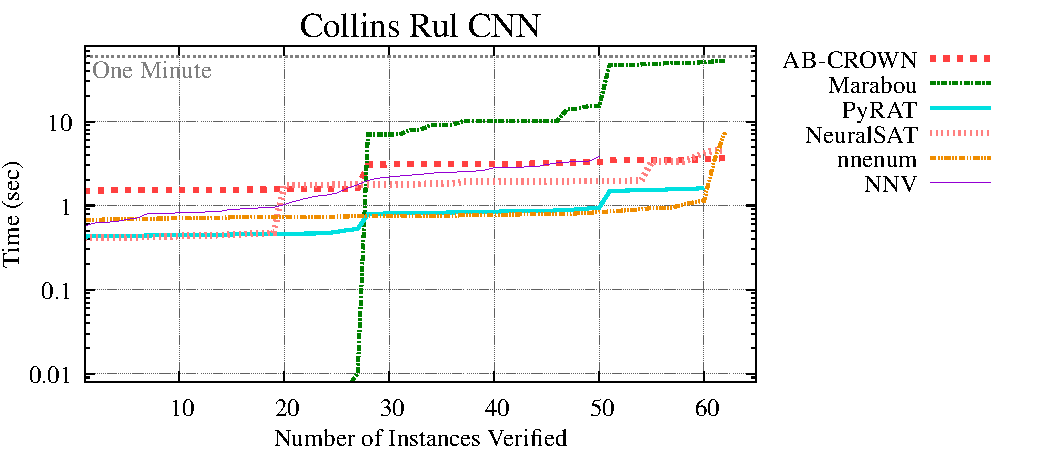
\includegraphics[width=\textwidth]{cactus/2023_collins_rul_cnn.pdf}}
\caption{Cactus Plot for Collins Rul CNN.}
\label{fig:quantPic}
\end{figure}


% Category 2023_dist_shift (single_overhead=True):

\begin{table}[h]
\begin{center}
\caption{Benchmark \texttt{2023-dist-shift}} \label{tab:cat_{cat}}
{\setlength{\tabcolsep}{2pt}
\begin{tabular}[h]{@{}llllllrr@{}}
\toprule
\textbf{\# ~} & \textbf{Tool} & \textbf{Verified} & \textbf{Falsified} & \textbf{Fastest} & \textbf{Penalty} & \textbf{Score} & \textbf{Percent}\\
\midrule
1 & $\alpha$-$\beta$-CROWN & 67 & 5 & 0 & 0 & 720 & 100.0\% \\
2 & PyRAT & 66 & 5 & 0 & 0 & 710 & 98.6\% \\
3 & NeuralSAT & 66 & 5 & 0 & 0 & 710 & 98.6\% \\
4 & Marabou & 55 & 5 & 0 & 0 & 600 & 83.3\% \\
5 & NNV & 0 & 4 & 0 & 0 & 40 & 5.6\% \\
\bottomrule
\end{tabular}
}
\end{center}
\end{table}



\begin{figure}[h]
\centerline{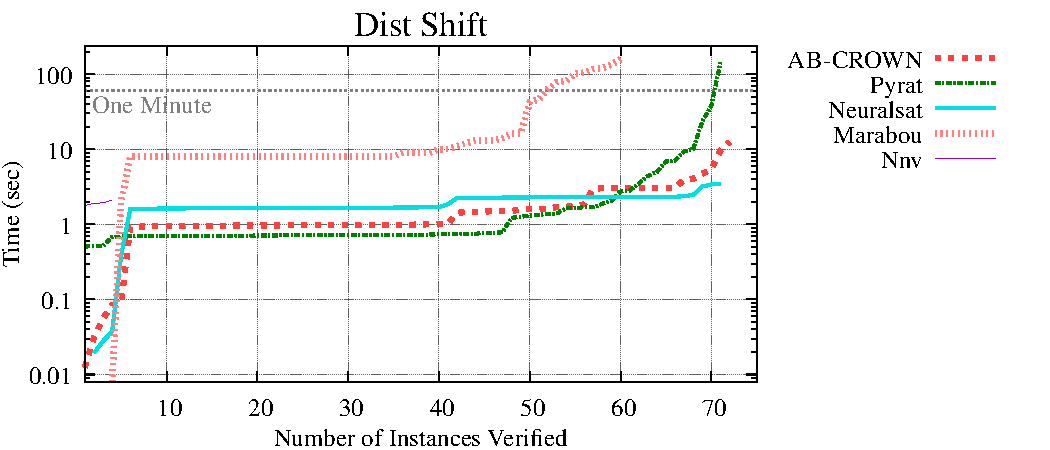
\includegraphics[width=\textwidth]{cactus/2023_dist_shift.pdf}}
\caption{Cactus Plot for Dist Shift.}
\label{fig:quantPic}
\end{figure}


% Category 2023_ml4acopf (single_overhead=True):

\begin{table}[h]
\begin{center}
\caption{Benchmark \texttt{2023-ml4acopf}} \label{tab:cat_{cat}}
{\setlength{\tabcolsep}{2pt}
\begin{tabular}[h]{@{}llllllrr@{}}
\toprule
\textbf{\# ~} & \textbf{Tool} & \textbf{Verified} & \textbf{Falsified} & \textbf{Fastest} & \textbf{Penalty} & \textbf{Score} & \textbf{Percent}\\
\midrule
1 & $\alpha$-$\beta$-CROWN & 18 & 1 & 0 & 0 & 190 & 100.0\% \\
\bottomrule
\end{tabular}
}
\end{center}
\end{table}



\begin{figure}[h]
\centerline{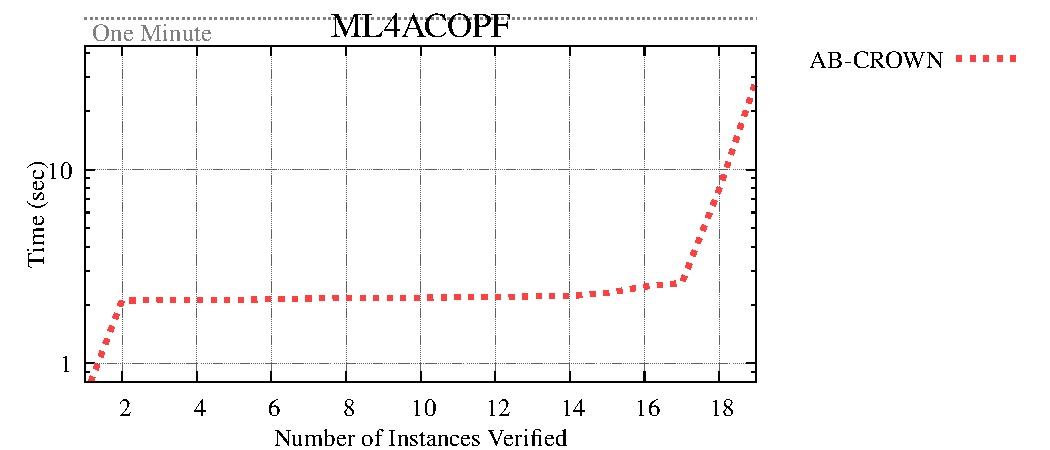
\includegraphics[width=\textwidth]{cactus/2023_ml4acopf.pdf}}
\caption{Cactus Plot for ML4ACOPF.}
\label{fig:quantPic}
\end{figure}


% Category 2023_nn4sys (single_overhead=True):

\begin{table}[h]
\begin{center}
\caption{Benchmark \texttt{2023-nn4sys}} \label{tab:cat_{cat}}
{\setlength{\tabcolsep}{2pt}
\begin{tabular}[h]{@{}llllllrr@{}}
\toprule
\textbf{\# ~} & \textbf{Tool} & \textbf{Verified} & \textbf{Falsified} & \textbf{Fastest} & \textbf{Penalty} & \textbf{Score} & \textbf{Percent}\\
\midrule
1 & $\alpha$-$\beta$-CROWN & 192 & 0 & 0 & 2 & 1620 & 100.0\% \\
2 & NeuralSAT & 81 & 0 & 0 & 2 & 510 & 31.5\% \\
3 & Marabou & 33 & 0 & 0 & 1 & 180 & 11.1\% \\
4 & PyRAT & 38 & 0 & 0 & 2 & 80 & 4.9\% \\
5 & nnenum & 20 & 0 & 0 & 2 & -100 & 0\% \\
6 & NNV & 0 & 2 & 0 & 8 & -1180 & 0\% \\
\bottomrule
\end{tabular}
}
\end{center}
\end{table}



\begin{figure}[h]
\centerline{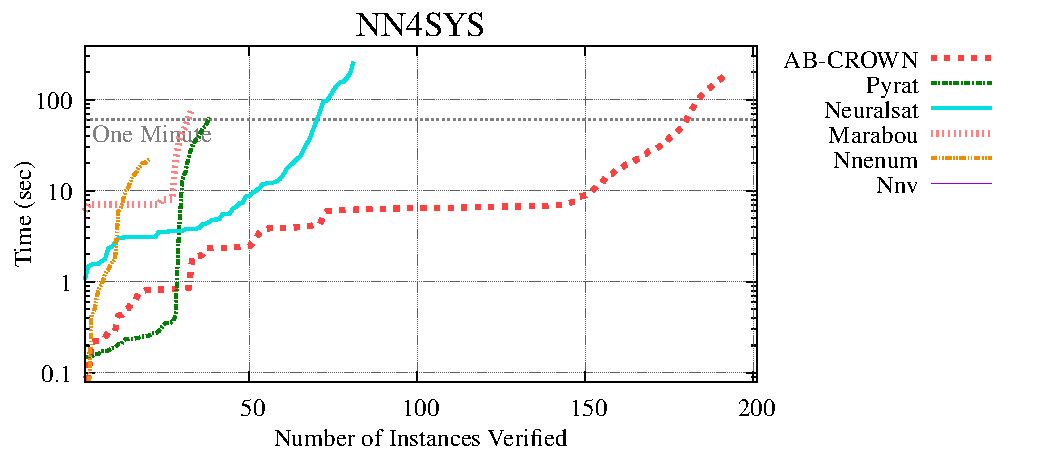
\includegraphics[width=\textwidth]{cactus/2023_nn4sys.pdf}}
\caption{Cactus Plot for NN4SYS.}
\label{fig:quantPic}
\end{figure}


% Category 2023_tllverifybench (single_overhead=True):

\begin{table}[h]
\begin{center}
\caption{Benchmark \texttt{2023-tllverifybench}} \label{tab:cat_{cat}}
{\setlength{\tabcolsep}{2pt}
\begin{tabular}[h]{@{}llllllrr@{}}
\toprule
\textbf{\# ~} & \textbf{Tool} & \textbf{Verified} & \textbf{Falsified} & \textbf{Fastest} & \textbf{Penalty} & \textbf{Score} & \textbf{Percent}\\
\midrule
1 & NeuralSAT & 15 & 17 & 0 & 0 & 320 & 100.0\% \\
2 & FastBATLLNN & 15 & 17 & 0 & 0 & 320 & 100.0\% \\
3 & $\alpha$-$\beta$-CROWN & 15 & 17 & 0 & 0 & 320 & 100.0\% \\
4 & PyRAT & 10 & 12 & 0 & 0 & 220 & 68.8\% \\
5 & Marabou & 5 & 17 & 0 & 0 & 220 & 68.8\% \\
6 & nnenum & 2 & 16 & 0 & 0 & 180 & 56.2\% \\
7 & NNV & 1 & 16 & 0 & 0 & 170 & 53.1\% \\
\bottomrule
\end{tabular}
}
\end{center}
\end{table}



\begin{figure}[h]
\centerline{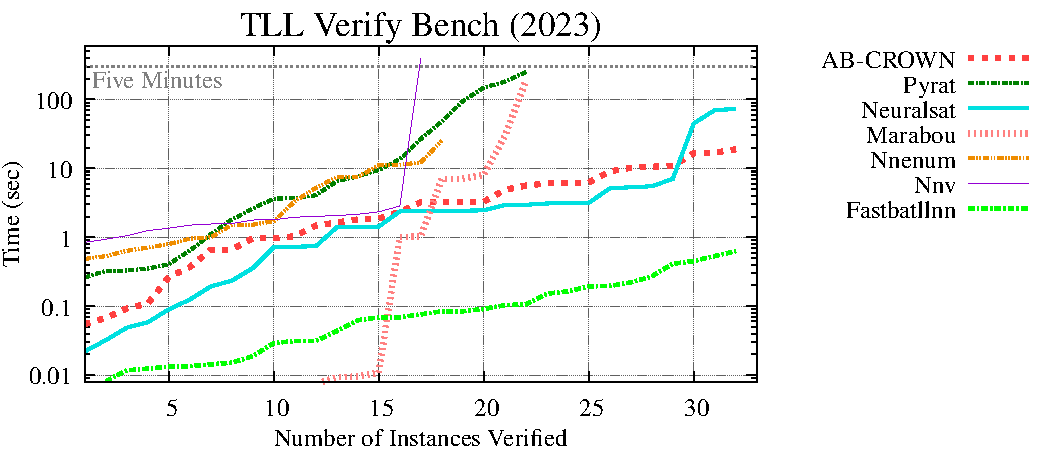
\includegraphics[width=\textwidth]{cactus/2023_tllverifybench.pdf}}
\caption{Cactus Plot for TLL Verify Bench (2023).}
\label{fig:quantPic}
\end{figure}


% Category 2023_traffic_signs_recognition (single_overhead=True):

\begin{table}[h]
\begin{center}
\caption{Benchmark \texttt{2023-traffic-signs-recognition}} \label{tab:cat_{cat}}
{\setlength{\tabcolsep}{2pt}
\begin{tabular}[h]{@{}llllllrr@{}}
\toprule
\textbf{\# ~} & \textbf{Tool} & \textbf{Verified} & \textbf{Falsified} & \textbf{Fastest} & \textbf{Penalty} & \textbf{Score} & \textbf{Percent}\\
\midrule
1 & Marabou & 0 & 18 & 0 & 1 & 30 & 100.0\% \\
2 & PyRAT & 0 & 7 & 0 & 1 & -80 & 0\% \\
3 & NeuralSAT & 0 & 31 & 0 & 4 & -290 & 0\% \\
4 & $\alpha$-$\beta$-CROWN & 0 & 39 & 0 & 3 & -60 & 0\% \\
\bottomrule
\end{tabular}
}
\end{center}
\end{table}



\begin{figure}[h]
\centerline{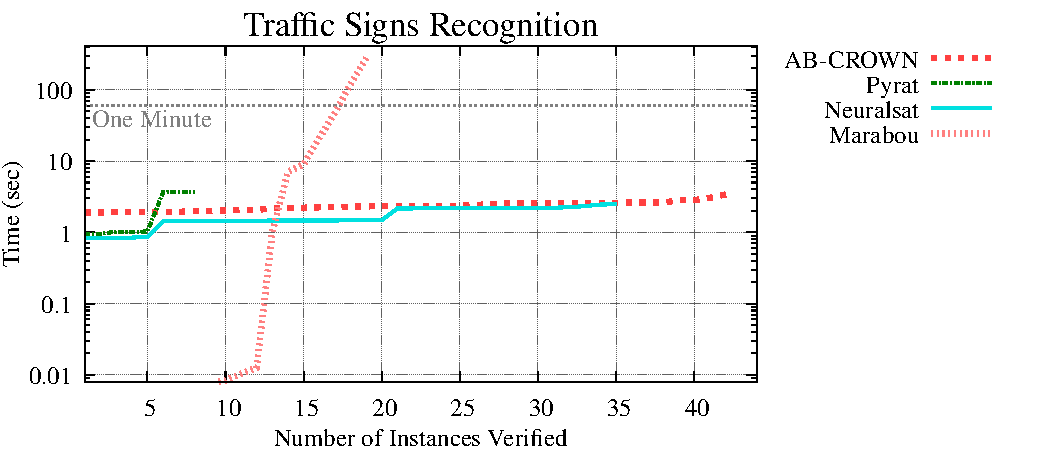
\includegraphics[width=\textwidth]{cactus/2023_traffic_signs_recognition.pdf}}
\caption{Cactus Plot for Traffic Signs Recognition.}
\label{fig:quantPic}
\end{figure}


% Category 2023_vggnet16 (single_overhead=True):

\begin{table}[h]
\begin{center}
\caption{Benchmark \texttt{2023-vggnet16}} \label{tab:cat_{cat}}
{\setlength{\tabcolsep}{2pt}
\begin{tabular}[h]{@{}llllllrr@{}}
\toprule
\textbf{\# ~} & \textbf{Tool} & \textbf{Verified} & \textbf{Falsified} & \textbf{Fastest} & \textbf{Penalty} & \textbf{Score} & \textbf{Percent}\\
\midrule
1 & $\alpha$-$\beta$-CROWN & 15 & 0 & 0 & 0 & 150 & 100.0\% \\
2 & nnenum & 14 & 0 & 0 & 0 & 140 & 93.3\% \\
3 & PyRAT & 13 & 1 & 0 & 0 & 140 & 93.3\% \\
4 & NeuralSAT & 5 & 1 & 0 & 0 & 60 & 40.0\% \\
5 & Marabou & 2 & 1 & 0 & 0 & 30 & 20.0\% \\
\bottomrule
\end{tabular}
}
\end{center}
\end{table}



\begin{figure}[h]
\centerline{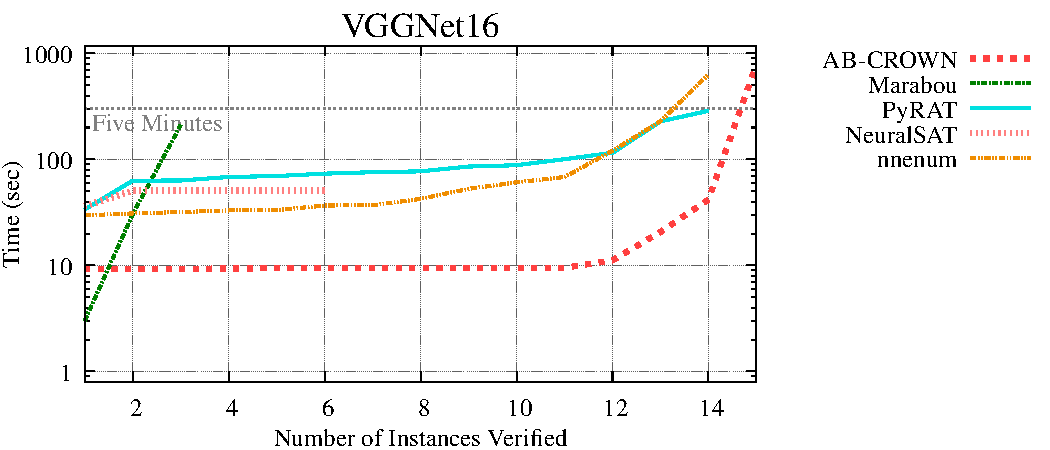
\includegraphics[width=\textwidth]{cactus/2023_vggnet16.pdf}}
\caption{Cactus Plot for VGGNet16.}
\label{fig:quantPic}
\end{figure}


% Category 2023_vit (single_overhead=True):

\begin{table}[h]
\begin{center}
\caption{Benchmark \texttt{2023-vit}} \label{tab:cat_{cat}}
{\setlength{\tabcolsep}{2pt}
\begin{tabular}[h]{@{}llllllrr@{}}
\toprule
\textbf{\# ~} & \textbf{Tool} & \textbf{Verified} & \textbf{Falsified} & \textbf{Fastest} & \textbf{Penalty} & \textbf{Score} & \textbf{Percent}\\
\midrule
1 & Marabou & 200 & 0 & 0 & 0 & 2000 & 100.0\% \\
2 & $\alpha$-$\beta$-CROWN & 79 & 0 & 0 & 0 & 790 & 39.5\% \\
\bottomrule
\end{tabular}
}
\end{center}
\end{table}



\begin{figure}[h]
\centerline{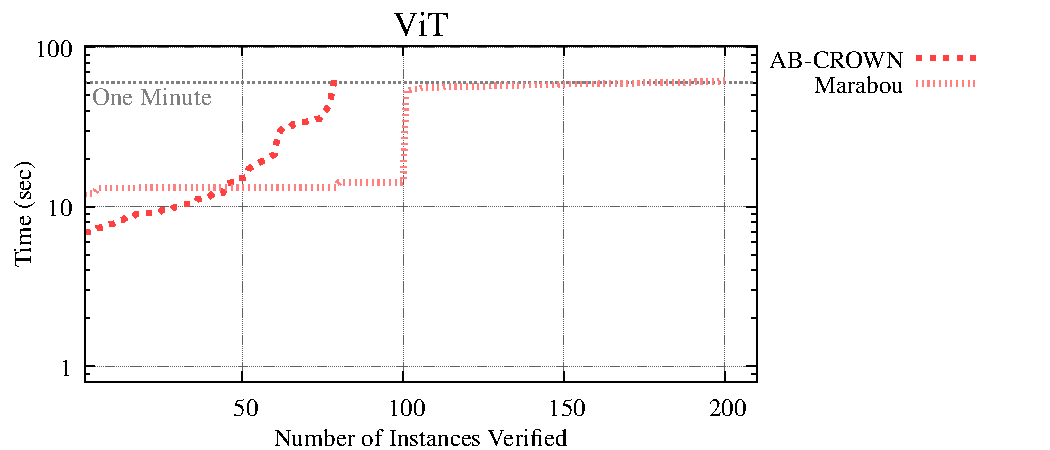
\includegraphics[width=\textwidth]{cactus/2023_vit.pdf}}
\caption{Cactus Plot for ViT.}
\label{fig:quantPic}
\end{figure}



\clearpage
\section{Unscored Benchmarks}

% Category 2022_carvana_unet_2022 (single_overhead=True):

\begin{table}[h]
\begin{center}
\caption{Benchmark \texttt{2022-carvana-unet-2022}} \label{tab:cat_{cat}}
{\setlength{\tabcolsep}{2pt}
\begin{tabular}[h]{@{}llllllrr@{}}
\toprule
\textbf{\# ~} & \textbf{Tool} & \textbf{Verified} & \textbf{Falsified} & \textbf{Fastest} & \textbf{Penalty} & \textbf{Score} & \textbf{Percent}\\
\midrule
1 & $\alpha$-$\beta$-CROWN & 39 & 0 & 0 & 0 & 390 & 100.0\% \\
\bottomrule
\end{tabular}
}
\end{center}
\end{table}



\begin{figure}[h]
\centerline{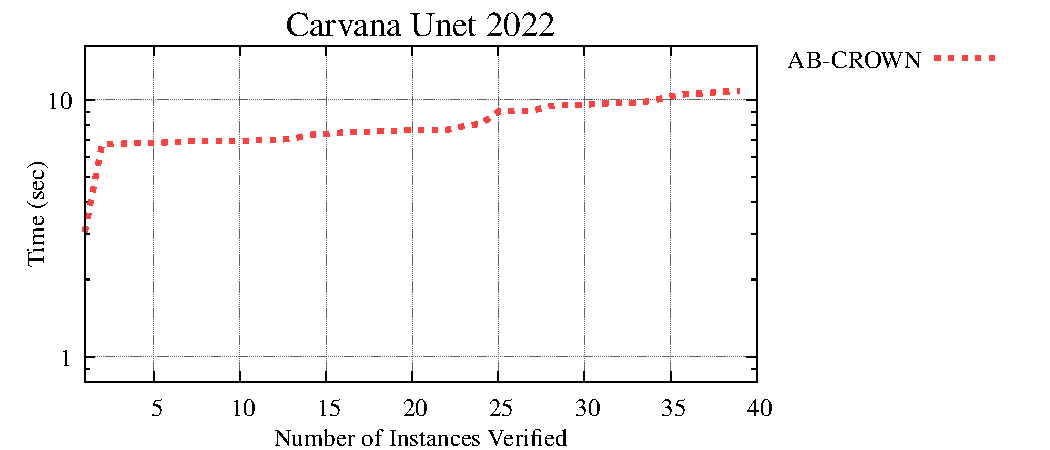
\includegraphics[width=\textwidth]{cactus/2022_carvana_unet_2022.pdf}}
\caption{Cactus Plot for Carvana Unet 2022.}
\label{fig:quantPic}
\end{figure}


% Category 2022_cifar100_tinyimagenet_resnet (single_overhead=True):

\begin{table}[h]
\begin{center}
\caption{Benchmark \texttt{2022-cifar100-tinyimagenet-resnet}} \label{tab:cat_{cat}}
{\setlength{\tabcolsep}{2pt}
\begin{tabular}[h]{@{}llllllrr@{}}
\toprule
\textbf{\# ~} & \textbf{Tool} & \textbf{Verified} & \textbf{Falsified} & \textbf{Fastest} & \textbf{Penalty} & \textbf{Score} & \textbf{Percent}\\
\midrule
1 & $\alpha$-$\beta$-CROWN & 69 & 3 & 0 & 0 & 720 & 100.0\% \\
2 & NeuralSAT & 56 & 3 & 0 & 0 & 590 & 81.9\% \\
\bottomrule
\end{tabular}
}
\end{center}
\end{table}



\begin{figure}[h]
\centerline{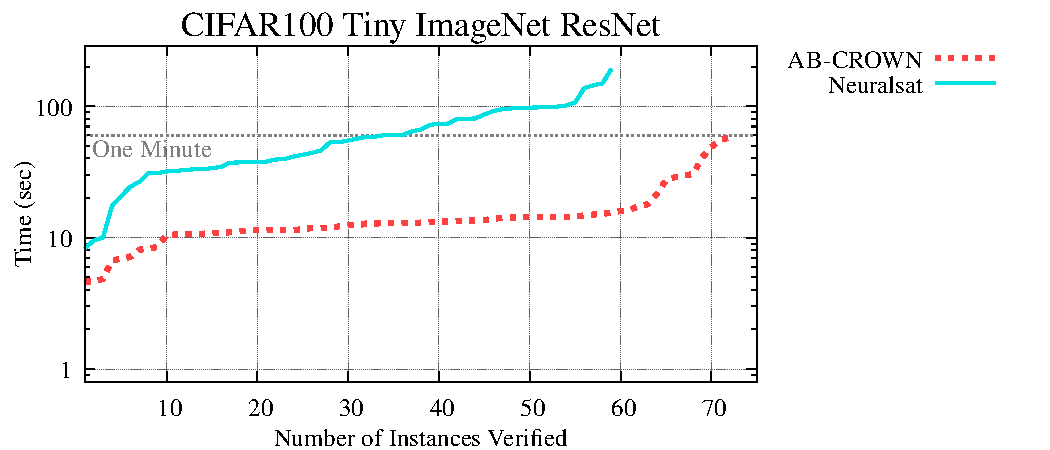
\includegraphics[width=\textwidth]{cactus/2022_cifar100_tinyimagenet_resnet.pdf}}
\caption{Cactus Plot for CIFAR100 Tiny ImageNet ResNet.}
\label{fig:quantPic}
\end{figure}


% Category 2022_cifar2020 (single_overhead=True):

\begin{table}[h]
\begin{center}
\caption{Benchmark \texttt{2022-cifar2020}} \label{tab:cat_{cat}}
{\setlength{\tabcolsep}{2pt}
\begin{tabular}[h]{@{}llllllrr@{}}
\toprule
\textbf{\# ~} & \textbf{Tool} & \textbf{Verified} & \textbf{Falsified} & \textbf{Fastest} & \textbf{Penalty} & \textbf{Score} & \textbf{Percent}\\
\midrule
1 & NeuralSAT & 148 & 42 & 0 & 0 & 1900 & 100.0\% \\
2 & $\alpha$-$\beta$-CROWN & 148 & 41 & 0 & 0 & 1890 & 99.5\% \\
3 & PyRAT & 96 & 39 & 0 & 0 & 1350 & 71.1\% \\
4 & nnenum & 66 & 19 & 0 & 0 & 850 & 44.7\% \\
5 & NNV & 32 & 6 & 0 & 0 & 380 & 20.0\% \\
\bottomrule
\end{tabular}
}
\end{center}
\end{table}



\begin{figure}[h]
\centerline{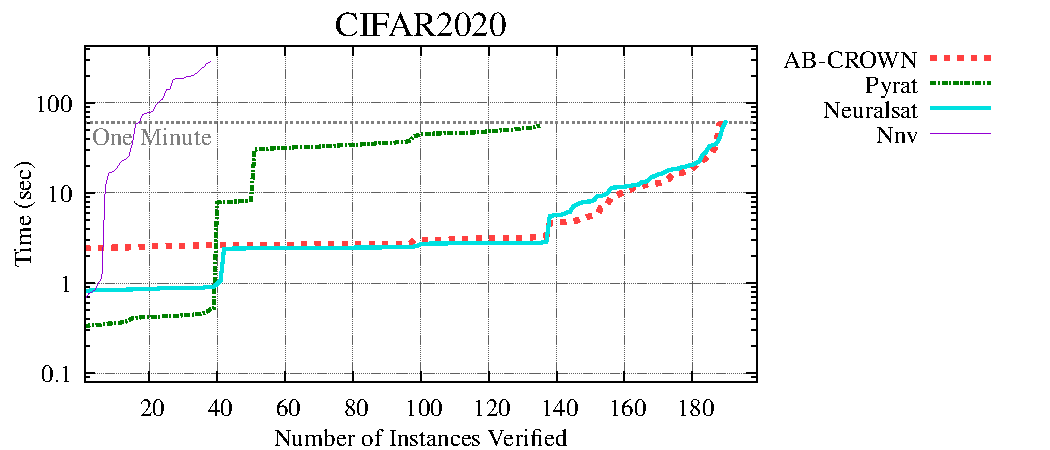
\includegraphics[width=\textwidth]{cactus/2022_cifar2020.pdf}}
\caption{Cactus Plot for CIFAR2020.}
\label{fig:quantPic}
\end{figure}


% Category 2022_cifar_biasfield (single_overhead=True):

\begin{table}[h]
\begin{center}
\caption{Benchmark \texttt{2022-cifar-biasfield}} \label{tab:cat_{cat}}
{\setlength{\tabcolsep}{2pt}
\begin{tabular}[h]{@{}llllllrr@{}}
\toprule
\textbf{\# ~} & \textbf{Tool} & \textbf{Verified} & \textbf{Falsified} & \textbf{Fastest} & \textbf{Penalty} & \textbf{Score} & \textbf{Percent}\\
\midrule
1 & $\alpha$-$\beta$-CROWN & 68 & 1 & 0 & 0 & 690 & 100.0\% \\
2 & NeuralSAT & 67 & 1 & 0 & 0 & 680 & 98.6\% \\
3 & PyRAT & 51 & 1 & 0 & 0 & 520 & 75.4\% \\
4 & nnenum & 18 & 0 & 0 & 0 & 180 & 26.1\% \\
\bottomrule
\end{tabular}
}
\end{center}
\end{table}



\begin{figure}[h]
\centerline{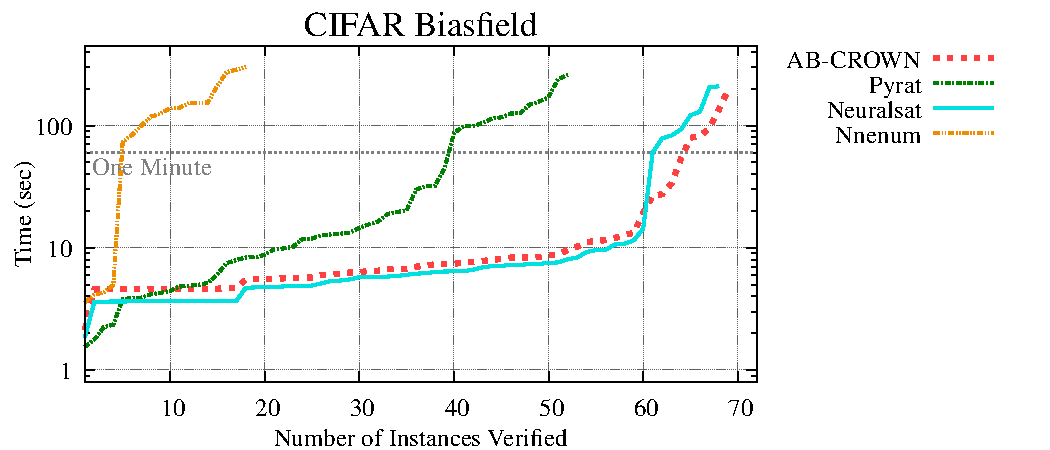
\includegraphics[width=\textwidth]{cactus/2022_cifar_biasfield.pdf}}
\caption{Cactus Plot for CIFAR Biasfield.}
\label{fig:quantPic}
\end{figure}


% Category 2022_mnist_fc (single_overhead=True):

\begin{table}[h]
\begin{center}
\caption{Benchmark \texttt{2022-mnist-fc}} \label{tab:cat_{cat}}
{\setlength{\tabcolsep}{2pt}
\begin{tabular}[h]{@{}llllllrr@{}}
\toprule
\textbf{\# ~} & \textbf{Tool} & \textbf{Verified} & \textbf{Falsified} & \textbf{Fastest} & \textbf{Penalty} & \textbf{Score} & \textbf{Percent}\\
\midrule
1 & $\alpha$-$\beta$-CROWN & 68 & 18 & 0 & 0 & 860 & 100.0\% \\
2 & NeuralSAT & 46 & 18 & 0 & 0 & 640 & 74.4\% \\
3 & nnenum & 48 & 11 & 0 & 0 & 590 & 68.6\% \\
4 & PyRAT & 35 & 16 & 0 & 0 & 510 & 59.3\% \\
5 & NNV & 30 & 4 & 0 & 0 & 340 & 39.5\% \\
\bottomrule
\end{tabular}
}
\end{center}
\end{table}



\begin{figure}[h]
\centerline{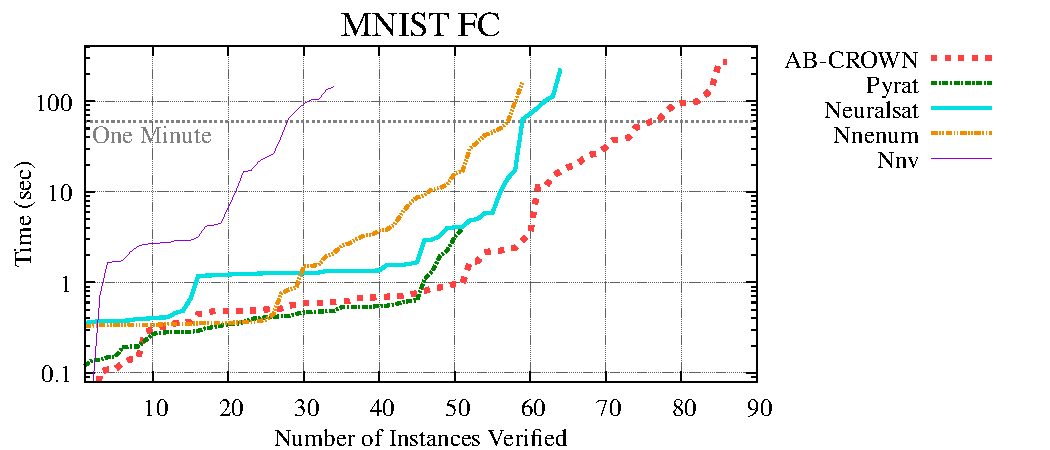
\includegraphics[width=\textwidth]{cactus/2022_mnist_fc.pdf}}
\caption{Cactus Plot for MNIST FC.}
\label{fig:quantPic}
\end{figure}


% Category 2022_nn4sys (single_overhead=True):

\begin{table}[h]
\begin{center}
\caption{Benchmark \texttt{2022-nn4sys}} \label{tab:cat_{cat}}
{\setlength{\tabcolsep}{2pt}
\begin{tabular}[h]{@{}llllllrr@{}}
\toprule
\textbf{\# ~} & \textbf{Tool} & \textbf{Verified} & \textbf{Falsified} & \textbf{Fastest} & \textbf{Penalty} & \textbf{Score} & \textbf{Percent}\\
\midrule
1 & $\alpha$-$\beta$-CROWN & 150 & 0 & 0 & 2 & 1200 & 100.0\% \\
2 & NeuralSAT & 76 & 0 & 0 & 2 & 460 & 38.3\% \\
3 & nnenum & 20 & 0 & 0 & 2 & -100 & 0\% \\
4 & PyRAT & 12 & 0 & 0 & 2 & -180 & 0\% \\
5 & NNV & 0 & 2 & 0 & 8 & -1180 & 0\% \\
\bottomrule
\end{tabular}
}
\end{center}
\end{table}



\begin{figure}[h]
\centerline{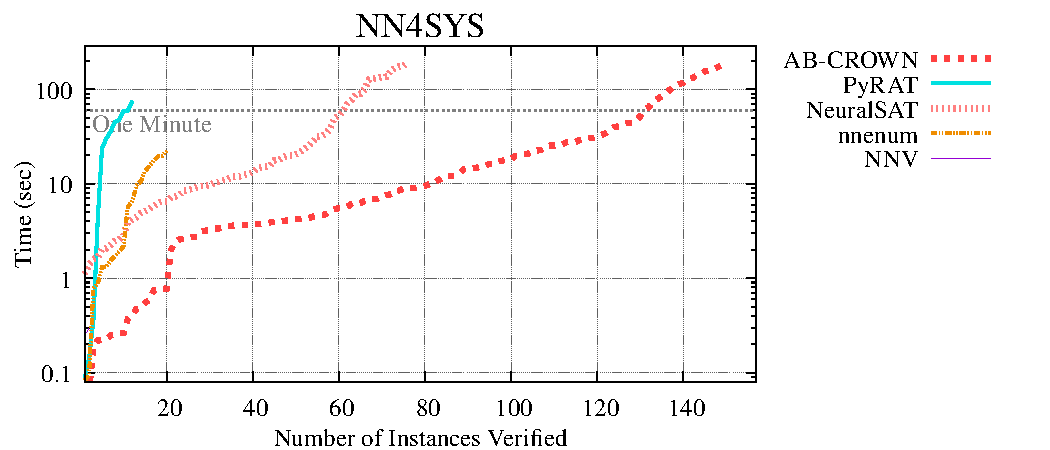
\includegraphics[width=\textwidth]{cactus/2022_nn4sys.pdf}}
\caption{Cactus Plot for NN4SYS.}
\label{fig:quantPic}
\end{figure}


% Category 2022_oval21 (single_overhead=True):

\begin{table}[h]
\begin{center}
\caption{Benchmark \texttt{2022-oval21}} \label{tab:cat_{cat}}
{\setlength{\tabcolsep}{2pt}
\begin{tabular}[h]{@{}llllllrr@{}}
\toprule
\textbf{\# ~} & \textbf{Tool} & \textbf{Verified} & \textbf{Falsified} & \textbf{Fastest} & \textbf{Penalty} & \textbf{Score} & \textbf{Percent}\\
\midrule
1 & $\alpha$-$\beta$-CROWN & 25 & 1 & 0 & 0 & 260 & 100.0\% \\
2 & NeuralSAT & 19 & 1 & 0 & 0 & 200 & 76.9\% \\
3 & nnenum & 3 & 1 & 0 & 0 & 40 & 15.4\% \\
4 & NNV & 4 & 0 & 0 & 0 & 40 & 15.4\% \\
5 & PyRAT & 1 & 1 & 0 & 0 & 20 & 7.7\% \\
\bottomrule
\end{tabular}
}
\end{center}
\end{table}



\begin{figure}[h]
\centerline{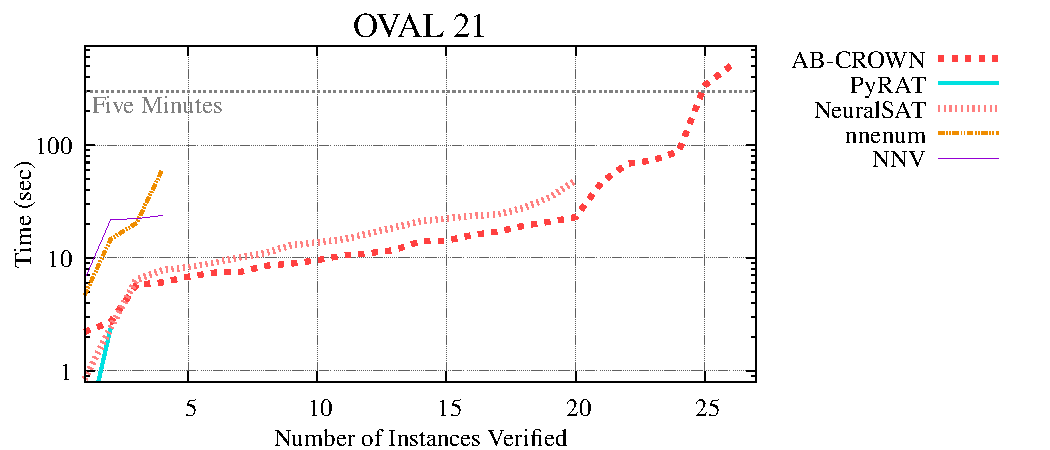
\includegraphics[width=\textwidth]{cactus/2022_oval21.pdf}}
\caption{Cactus Plot for OVAL 21.}
\label{fig:quantPic}
\end{figure}


% Category 2022_reach_prob_density (single_overhead=True):

\begin{table}[h]
\begin{center}
\caption{Benchmark \texttt{2022-reach-prob-density}} \label{tab:cat_{cat}}
{\setlength{\tabcolsep}{2pt}
\begin{tabular}[h]{@{}llllllrr@{}}
\toprule
\textbf{\# ~} & \textbf{Tool} & \textbf{Verified} & \textbf{Falsified} & \textbf{Fastest} & \textbf{Penalty} & \textbf{Score} & \textbf{Percent}\\
\midrule
1 & nnenum & 22 & 14 & 0 & 0 & 360 & 100.0\% \\
2 & $\alpha$-$\beta$-CROWN & 22 & 14 & 0 & 0 & 360 & 100.0\% \\
3 & NeuralSAT & 22 & 12 & 0 & 0 & 340 & 94.4\% \\
4 & PyRAT & 17 & 7 & 0 & 0 & 240 & 66.7\% \\
5 & NNV & 9 & 0 & 0 & 0 & 90 & 25.0\% \\
\bottomrule
\end{tabular}
}
\end{center}
\end{table}



\begin{figure}[h]
\centerline{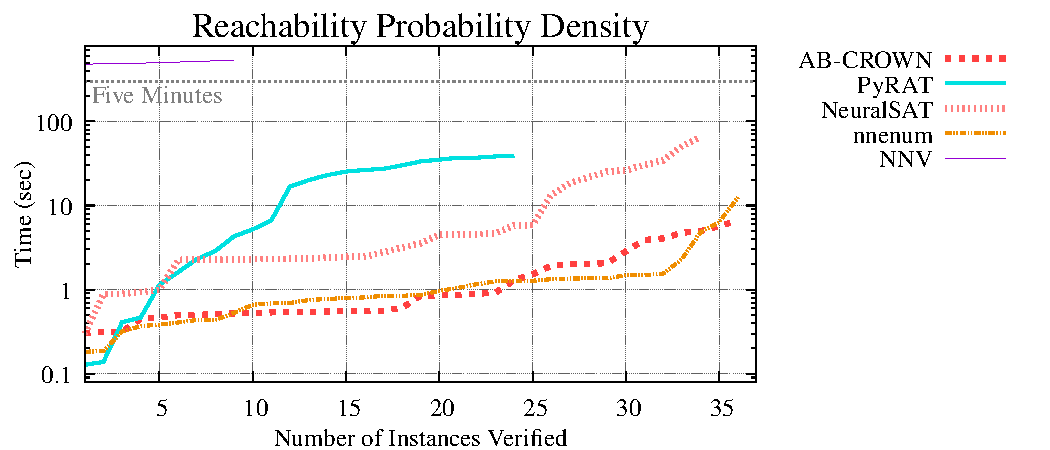
\includegraphics[width=\textwidth]{cactus/2022_reach_prob_density.pdf}}
\caption{Cactus Plot for Reachability Probability Density.}
\label{fig:quantPic}
\end{figure}


% Category 2022_rl_benchmarks (single_overhead=True):

\begin{table}[h]
\begin{center}
\caption{Benchmark \texttt{2022-rl-benchmarks}} \label{tab:cat_{cat}}
{\setlength{\tabcolsep}{2pt}
\begin{tabular}[h]{@{}llllllrr@{}}
\toprule
\textbf{\# ~} & \textbf{Tool} & \textbf{Verified} & \textbf{Falsified} & \textbf{Fastest} & \textbf{Penalty} & \textbf{Score} & \textbf{Percent}\\
\midrule
1 & NeuralSAT & 193 & 103 & 0 & 0 & 2960 & 100.0\% \\
2 & $\alpha$-$\beta$-CROWN & 193 & 103 & 0 & 0 & 2960 & 100.0\% \\
3 & nnenum & 191 & 103 & 0 & 0 & 2940 & 99.3\% \\
4 & NNV & 177 & 90 & 0 & 0 & 2670 & 90.2\% \\
5 & PyRAT & 191 & 96 & 0 & 3 & 2420 & 81.8\% \\
\bottomrule
\end{tabular}
}
\end{center}
\end{table}



\begin{figure}[h]
\centerline{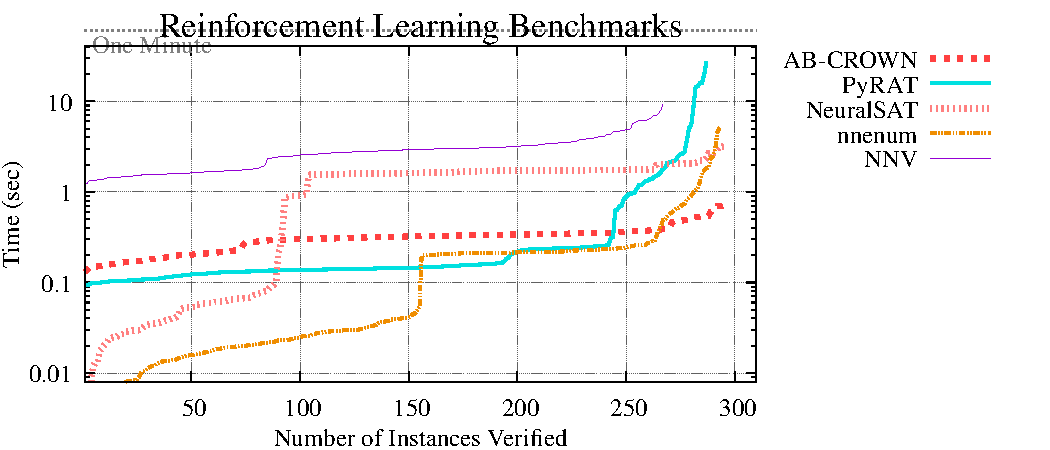
\includegraphics[width=\textwidth]{cactus/2022_rl_benchmarks.pdf}}
\caption{Cactus Plot for Reinforcement Learning Benchmarks.}
\label{fig:quantPic}
\end{figure}


% Category 2022_sri_resnet_a (single_overhead=True):

\begin{table}[h]
\begin{center}
\caption{Benchmark \texttt{2022-sri-resnet-a}} \label{tab:cat_{cat}}
{\setlength{\tabcolsep}{2pt}
\begin{tabular}[h]{@{}llllllrr@{}}
\toprule
\textbf{\# ~} & \textbf{Tool} & \textbf{Verified} & \textbf{Falsified} & \textbf{Fastest} & \textbf{Penalty} & \textbf{Score} & \textbf{Percent}\\
\midrule
1 & $\alpha$-$\beta$-CROWN & 20 & 12 & 0 & 0 & 320 & 100.0\% \\
2 & NeuralSAT & 18 & 12 & 0 & 0 & 300 & 93.8\% \\
3 & PyRAT & 5 & 11 & 0 & 0 & 160 & 50.0\% \\
\bottomrule
\end{tabular}
}
\end{center}
\end{table}



\begin{figure}[h]
\centerline{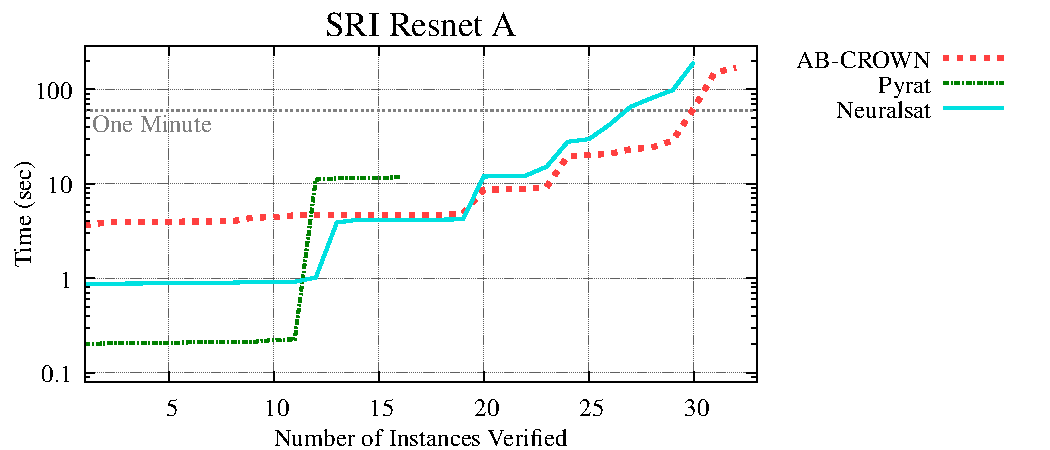
\includegraphics[width=\textwidth]{cactus/2022_sri_resnet_a.pdf}}
\caption{Cactus Plot for SRI Resnet A.}
\label{fig:quantPic}
\end{figure}


% Category 2022_sri_resnet_b (single_overhead=True):

\begin{table}[h]
\begin{center}
\caption{Benchmark \texttt{2022-sri-resnet-b}} \label{tab:cat_{cat}}
{\setlength{\tabcolsep}{2pt}
\begin{tabular}[h]{@{}llllllrr@{}}
\toprule
\textbf{\# ~} & \textbf{Tool} & \textbf{Verified} & \textbf{Falsified} & \textbf{Fastest} & \textbf{Penalty} & \textbf{Score} & \textbf{Percent}\\
\midrule
1 & NeuralSAT & 28 & 11 & 0 & 0 & 390 & 100.0\% \\
2 & $\alpha$-$\beta$-CROWN & 28 & 11 & 0 & 0 & 390 & 100.0\% \\
3 & PyRAT & 13 & 11 & 0 & 0 & 240 & 61.5\% \\
4 & NNV & 1 & 0 & 0 & 1 & -140 & 0\% \\
\bottomrule
\end{tabular}
}
\end{center}
\end{table}



\begin{figure}[h]
\centerline{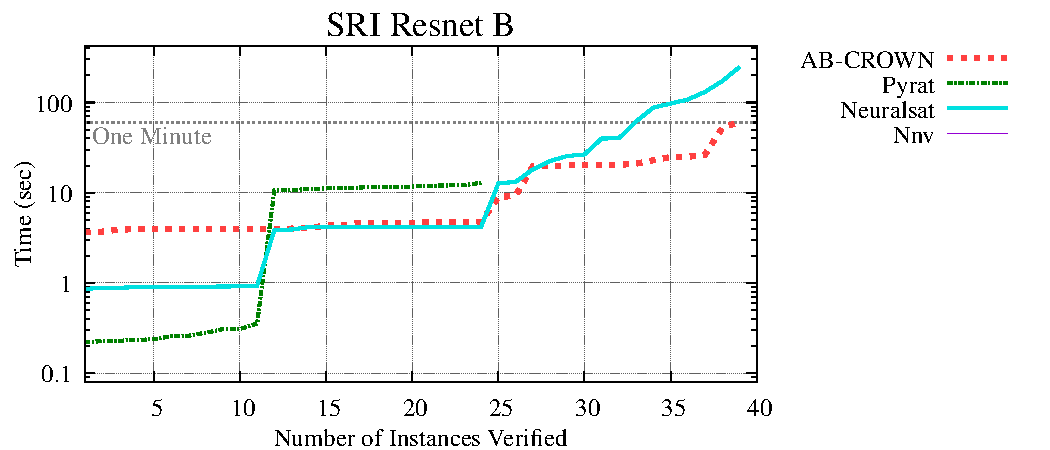
\includegraphics[width=\textwidth]{cactus/2022_sri_resnet_b.pdf}}
\caption{Cactus Plot for SRI Resnet B.}
\label{fig:quantPic}
\end{figure}


% Category 2022_tllverifybench (single_overhead=True):

\begin{table}[h]
\begin{center}
\caption{Benchmark \texttt{2022-tllverifybench}} \label{tab:cat_{cat}}
{\setlength{\tabcolsep}{2pt}
\begin{tabular}[h]{@{}llllllrr@{}}
\toprule
\textbf{\# ~} & \textbf{Tool} & \textbf{Verified} & \textbf{Falsified} & \textbf{Fastest} & \textbf{Penalty} & \textbf{Score} & \textbf{Percent}\\
\midrule
1 & NeuralSAT & 11 & 21 & 0 & 0 & 320 & 100.0\% \\
2 & FastBATLLNN & 11 & 21 & 0 & 0 & 320 & 100.0\% \\
3 & $\alpha$-$\beta$-CROWN & 11 & 21 & 0 & 0 & 320 & 100.0\% \\
4 & PyRAT & 9 & 17 & 0 & 0 & 260 & 81.2\% \\
5 & nnenum & 1 & 21 & 0 & 0 & 220 & 68.8\% \\
6 & NNV & 0 & 21 & 0 & 0 & 210 & 65.6\% \\
\bottomrule
\end{tabular}
}
\end{center}
\end{table}



\begin{figure}[h]
\centerline{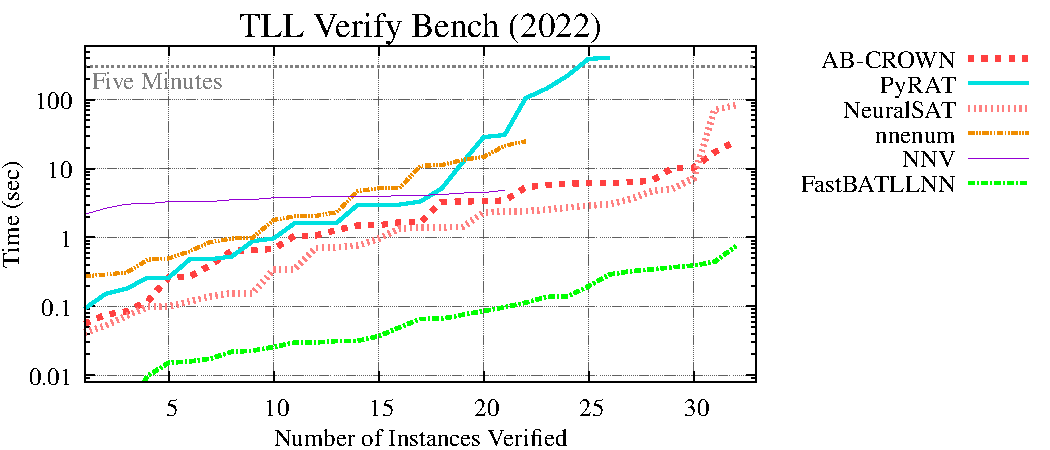
\includegraphics[width=\textwidth]{cactus/2022_tllverifybench.pdf}}
\caption{Cactus Plot for TLL Verify Bench (2022).}
\label{fig:quantPic}
\end{figure}


% Category 2022_vggnet16_2022 (single_overhead=True):

\begin{table}[h]
\begin{center}
\caption{Benchmark \texttt{2022-vggnet16-2022}} \label{tab:cat_{cat}}
{\setlength{\tabcolsep}{2pt}
\begin{tabular}[h]{@{}llllllrr@{}}
\toprule
\textbf{\# ~} & \textbf{Tool} & \textbf{Verified} & \textbf{Falsified} & \textbf{Fastest} & \textbf{Penalty} & \textbf{Score} & \textbf{Percent}\\
\midrule
1 & $\alpha$-$\beta$-CROWN & 14 & 1 & 0 & 0 & 150 & 100.0\% \\
2 & nnenum & 11 & 1 & 0 & 0 & 120 & 80.0\% \\
3 & PyRAT & 9 & 1 & 0 & 0 & 100 & 66.7\% \\
4 & NeuralSAT & 5 & 1 & 0 & 0 & 60 & 40.0\% \\
\bottomrule
\end{tabular}
}
\end{center}
\end{table}



\begin{figure}[h]
\centerline{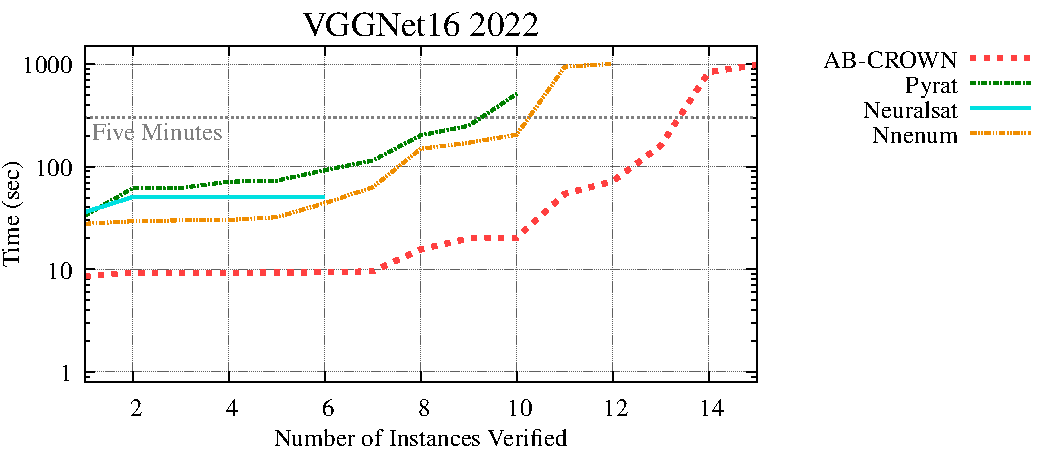
\includegraphics[width=\textwidth]{cactus/2022_vggnet16_2022.pdf}}
\caption{Cactus Plot for VGGNet16 2022.}
\label{fig:quantPic}
\end{figure}


% Category 2023_cctsdb_yolo (single_overhead=True):

\begin{table}[h]
\begin{center}
\caption{Benchmark \texttt{2023-cctsdb-yolo}} \label{tab:cat_{cat}}
{\setlength{\tabcolsep}{2pt}
\begin{tabular}[h]{@{}llllllrr@{}}
\toprule
\textbf{\# ~} & \textbf{Tool} & \textbf{Verified} & \textbf{Falsified} & \textbf{Fastest} & \textbf{Penalty} & \textbf{Score} & \textbf{Percent}\\
\midrule
1 & $\alpha$-$\beta$-CROWN & 11 & 28 & 0 & 0 & 390 & 100.0\% \\
\bottomrule
\end{tabular}
}
\end{center}
\end{table}



\begin{figure}[h]
\centerline{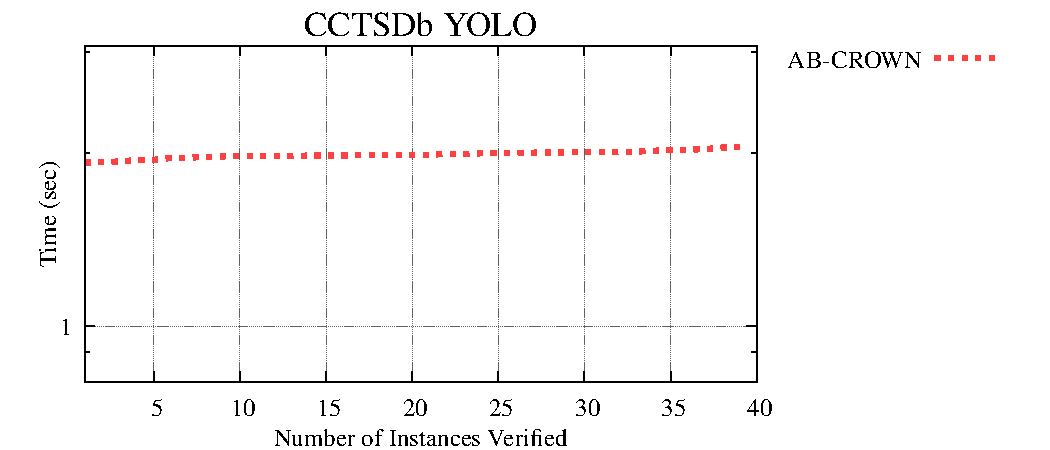
\includegraphics[width=\textwidth]{cactus/2023_cctsdb_yolo.pdf}}
\caption{Cactus Plot for CCTSDb YOLO.}
\label{fig:quantPic}
\end{figure}


% Category 2023_collins_yolo_robustness (single_overhead=True):

\begin{table}[h]
\begin{center}
\caption{Benchmark \texttt{2023-collins-yolo-robustness}} \label{tab:cat_{cat}}
{\setlength{\tabcolsep}{2pt}
\begin{tabular}[h]{@{}llllllrr@{}}
\toprule
\textbf{\# ~} & \textbf{Tool} & \textbf{Verified} & \textbf{Falsified} & \textbf{Fastest} & \textbf{Penalty} & \textbf{Score} & \textbf{Percent}\\
\midrule
1 & PyRAT & 0 & 6 & 0 & 0 & 60 & 100.0\% \\
2 & $\alpha$-$\beta$-CROWN & 0 & 6 & 0 & 0 & 60 & 100.0\% \\
\bottomrule
\end{tabular}
}
\end{center}
\end{table}



\begin{figure}[h]
\centerline{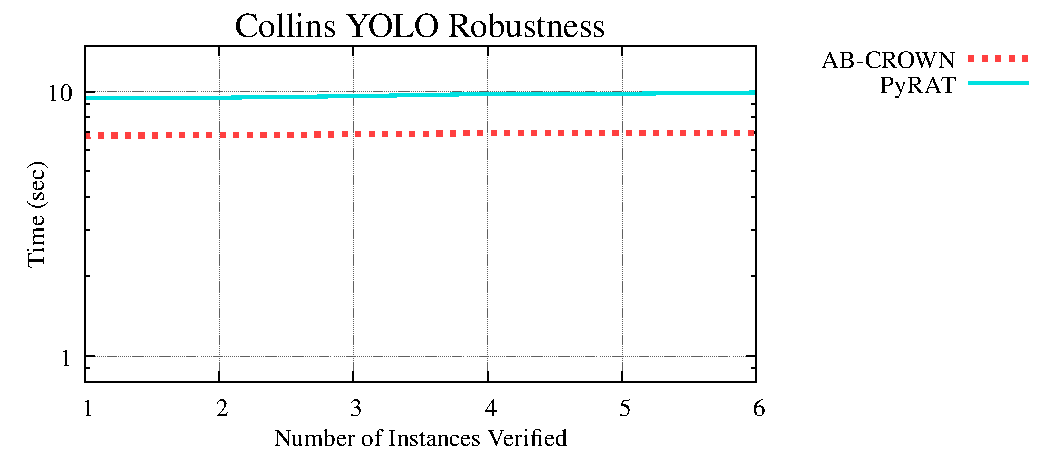
\includegraphics[width=\textwidth]{cactus/2023_collins_yolo_robustness.pdf}}
\caption{Cactus Plot for Collins YOLO Robustness.}
\label{fig:quantPic}
\end{figure}


% Category 2023_metaroom (single_overhead=True):

\begin{table}[h]
\begin{center}
\caption{Benchmark \texttt{2023-metaroom}} \label{tab:cat_{cat}}
{\setlength{\tabcolsep}{2pt}
\begin{tabular}[h]{@{}llllllrr@{}}
\toprule
\textbf{\# ~} & \textbf{Tool} & \textbf{Verified} & \textbf{Falsified} & \textbf{Fastest} & \textbf{Penalty} & \textbf{Score} & \textbf{Percent}\\
\midrule
1 & $\alpha$-$\beta$-CROWN & 94 & 5 & 0 & 0 & 990 & 100.0\% \\
2 & NeuralSAT & 92 & 5 & 0 & 0 & 970 & 98.0\% \\
3 & PyRAT & 93 & 2 & 0 & 0 & 950 & 96.0\% \\
4 & nnenum & 51 & 2 & 0 & 0 & 530 & 53.5\% \\
\bottomrule
\end{tabular}
}
\end{center}
\end{table}



\begin{figure}[h]
\centerline{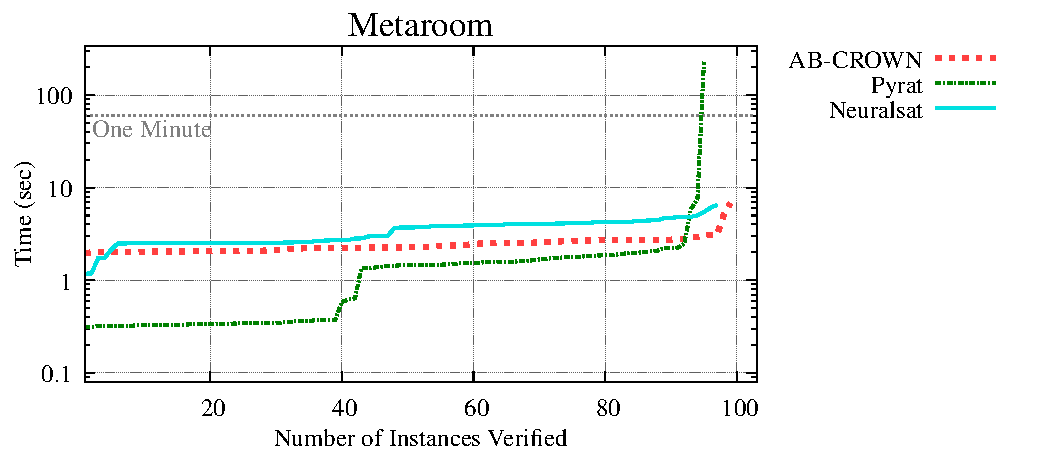
\includegraphics[width=\textwidth]{cactus/2023_metaroom.pdf}}
\caption{Cactus Plot for Metaroom.}
\label{fig:quantPic}
\end{figure}


% Category 2023_yolo (single_overhead=True):

\begin{table}[h]
\begin{center}
\caption{Benchmark \texttt{2023-yolo}} \label{tab:cat_{cat}}
{\setlength{\tabcolsep}{2pt}
\begin{tabular}[h]{@{}llllllrr@{}}
\toprule
\textbf{\# ~} & \textbf{Tool} & \textbf{Verified} & \textbf{Falsified} & \textbf{Fastest} & \textbf{Penalty} & \textbf{Score} & \textbf{Percent}\\
\midrule
1 & $\alpha$-$\beta$-CROWN & 63 & 0 & 0 & 0 & 630 & 100.0\% \\
2 & PyRAT & 41 & 0 & 0 & 0 & 410 & 65.1\% \\
3 & NNV & 0 & 0 & 0 & 41 & -6150 & 0\% \\
\bottomrule
\end{tabular}
}
\end{center}
\end{table}



\begin{figure}[h]
\centerline{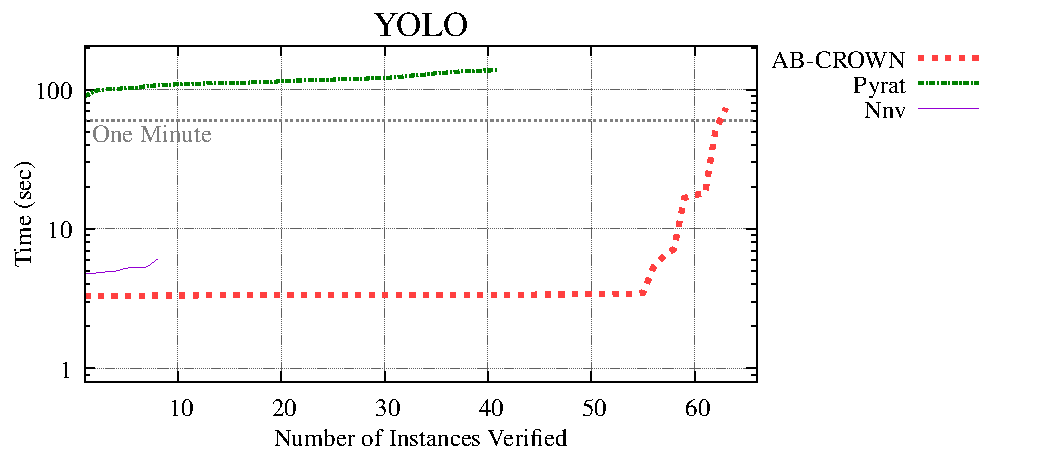
\includegraphics[width=\textwidth]{cactus/2023_yolo.pdf}}
\caption{Cactus Plot for YOLO.}
\label{fig:quantPic}
\end{figure}



\clearpage
\section{Stats}

%%%%%%%%%% Stats %%%%%%%%%%%

% Overhead:

\begin{table}[h]
\begin{center}
\caption{Overhead} \label{tab:overhead}
{\setlength{\tabcolsep}{2pt}
\begin{tabular}[h]{@{}llr@{}}
\toprule
\textbf{\# ~} & \textbf{Tool} & \textbf{Seconds}\\
\midrule
1 & Marabou & 0.2 \\
2 & Fastbatllnn & 0.5 \\
3 & Nnenum & 0.9 \\
4 & Cgdtest & 1.3 \\
5 & Peregrinn & 1.3 \\
6 & Debona & 2.0 \\
7 & Averinn & 3.1 \\
8 & Verinet & 3.4 \\
9 & Verapak & 4.6 \\
10 & $\alpha$,$\beta$ Crown & 6.7 \\
11 & MN BaB & 8.2 \\
\bottomrule
\end{tabular}
}
\end{center}
\end{table}



% Num Benchmarks Participated:

\begin{table}[h]
\begin{center}
\caption{Num Benchmarks Participated} \label{tab:stats0}
{\setlength{\tabcolsep}{2pt}
\begin{tabular}[h]{@{}llr@{}}
\toprule
\textbf{\# ~} & \textbf{Tool} & \textbf{Count}\\
\midrule
1 & Verinet & 13 \\
2 & MN BaB & 13 \\
3 & $\alpha$,$\beta$ Crown & 13 \\
4 & Cgdtest & 12 \\
5 & Nnenum & 9 \\
6 & Peregrinn & 7 \\
7 & Marabou & 6 \\
8 & Debona & 5 \\
9 & Verapak & 3 \\
10 & Fastbatllnn & 1 \\
11 & Averinn & 1 \\
\bottomrule
\end{tabular}
}
\end{center}
\end{table}



% Num Instances Verified:

\begin{table}[h]
\begin{center}
\caption{Num Instances Verified} \label{tab:stats1}
{\setlength{\tabcolsep}{2pt}
\begin{tabular}[h]{@{}llr@{}}
\toprule
\textbf{\# ~} & \textbf{Tool} & \textbf{Count}\\
\midrule
1 & $\alpha$,$\beta$ Crown & 950 \\
2 & MN BaB & 812 \\
3 & Verinet & 754 \\
4 & Nnenum & 515 \\
5 & Peregrinn & 478 \\
6 & Marabou & 450 \\
7 & Cgdtest & 405 \\
8 & Debona & 341 \\
9 & Verapak & 117 \\
10 & Averinn & 100 \\
11 & Fastbatllnn & 32 \\
\bottomrule
\end{tabular}
}
\end{center}
\end{table}



% Num SAT:

\begin{table}[h]
\begin{center}
\caption{Num SAT} \label{tab:stats2}
{\setlength{\tabcolsep}{2pt}
\begin{tabular}[h]{@{}llr@{}}
\toprule
\textbf{\# ~} & \textbf{Tool} & \textbf{Count}\\
\midrule
1 & Verinet & 228 \\
2 & MN BaB & 227 \\
3 & $\alpha$,$\beta$ Crown & 227 \\
4 & Nnenum & 196 \\
5 & Peregrinn & 191 \\
6 & Marabou & 148 \\
7 & Debona & 138 \\
8 & Cgdtest & 101 \\
9 & Fastbatllnn & 21 \\
10 & Averinn & 8 \\
11 & Verapak & 6 \\
\bottomrule
\end{tabular}
}
\end{center}
\end{table}



% Num UNSAT:

\begin{table}[h]
\begin{center}
\caption{Num UNSAT} \label{tab:stats3}
{\setlength{\tabcolsep}{2pt}
\begin{tabular}[h]{@{}llr@{}}
\toprule
\textbf{\# ~} & \textbf{Tool} & \textbf{Count}\\
\midrule
1 & $\alpha$,$\beta$ Crown & 723 \\
2 & MN BaB & 585 \\
3 & Verinet & 526 \\
4 & Nnenum & 319 \\
5 & Cgdtest & 304 \\
6 & Marabou & 302 \\
7 & Peregrinn & 287 \\
8 & Debona & 203 \\
9 & Verapak & 111 \\
10 & Averinn & 92 \\
11 & Fastbatllnn & 11 \\
\bottomrule
\end{tabular}
}
\end{center}
\end{table}



% Incorrect Results (or Missing CE):

\begin{table}[h]
\begin{center}
\caption{Incorrect Results (or Missing CE)} \label{tab:stats4}
{\setlength{\tabcolsep}{2pt}
\begin{tabular}[h]{@{}llr@{}}
\toprule
\textbf{\# ~} & \textbf{Tool} & \textbf{Count}\\
\midrule
1 & Cgdtest & 41 \\
2 & Verapak & 5 \\
3 & Marabou & 1 \\
4 & $\alpha$,$\beta$ Crown & 1 \\
\bottomrule
\end{tabular}
}
\end{center}
\end{table}




\clearpage
\section{Detailed Results}
% Long table of all results


\begin{center}
{\setlength{\tabcolsep}{1pt}
\scriptsize
\begin{longtable}{@{}llllllllll@{}}
\caption{\footnotesize Instance Runtimes. Fastest times are \textcolor{blue}{blue}. Second fastest are \textcolor{second}{green}. Penalties are red crosses (\textbf{\textcolor{red}{\ding{55}}}).} \label{tab:all_results} \\
\toprule
\textbf{Category} & \textbf{Id} & \textbf{Result} & \textbf{$\alpha$,$\beta$-C} & \textbf{PyRat} & \textbf{NSAT} & \textbf{Marab} & \textbf{NNen} & \textbf{NNV} & \textbf{FastBaT} \\
\midrule
\endhead
2022 Nn4sys & 0 & ~\textsc{unsat} & \textcolor{darkgray}{0.05} & \textcolor{darkgray}{0.09} & \textcolor{darkgray}{1.62} & - & \textcolor{darkgray}{0.11} & - & - \\
2022 Nn4sys & 1 & ~\textsc{unsat} & \textcolor{darkgray}{0.03} & \textcolor{darkgray}{0.14} & \textcolor{darkgray}{1.54} & - & \textcolor{darkgray}{0.10} & - & - \\
2022 Nn4sys & 2 & ~\textsc{sat} & ~~\textbf{\textcolor{red}{\ding{55}}} & ~~\textbf{\textcolor{red}{\ding{55}}} & ~~\textbf{\textcolor{red}{\ding{55}}} & - & ~~\textbf{\textcolor{red}{\ding{55}}} & \textcolor{darkgray}{0.05} & - \\
2022 Nn4sys & 3 & ~\textsc{sat} & ~~\textbf{\textcolor{red}{\ding{55}}} & ~~\textbf{\textcolor{red}{\ding{55}}} & ~~\textbf{\textcolor{red}{\ding{55}}} & - & ~~\textbf{\textcolor{red}{\ding{55}}} & \textcolor{darkgray}{$<$0.01} & - \\
2022 Nn4sys & 4 & ~\textsc{unsat} & \textcolor{darkgray}{0.23} & \textcolor{darkgray}{23.6} & \textcolor{darkgray}{1.07} & - & \textcolor{darkgray}{0.80} & ~~\textbf{\textcolor{red}{\ding{55}}} & - \\
2022 Nn4sys & 5 & ~\textsc{unsat} & \textcolor{darkgray}{0.25} & \textcolor{darkgray}{30.2} & \textcolor{darkgray}{2.20} & - & \textcolor{darkgray}{0.88} & ~~\textbf{\textcolor{red}{\ding{55}}} & - \\
2022 Nn4sys & 6 & ~\textsc{unsat} & \textcolor{darkgray}{0.17} & \textcolor{darkgray}{35.7} & \textcolor{darkgray}{2.03} & - & \textcolor{darkgray}{1.32} & ~~\textbf{\textcolor{red}{\ding{55}}} & - \\
2022 Nn4sys & 7 & ~\textsc{unsat} & \textcolor{darkgray}{0.21} & \textcolor{darkgray}{44.9} & \textcolor{darkgray}{2.43} & - & \textcolor{darkgray}{1.32} & ~~\textbf{\textcolor{red}{\ding{55}}} & - \\
2022 Nn4sys & 8 & ~\textsc{unsat} & \textcolor{darkgray}{0.21} & \textcolor{darkgray}{47.5} & \textcolor{darkgray}{1.36} & - & \textcolor{darkgray}{1.56} & ~~\textbf{\textcolor{red}{\ding{55}}} & - \\
2022 Nn4sys & 9 & ~\textsc{unsat} & \textcolor{darkgray}{0.25} & \textcolor{darkgray}{59.6} & \textcolor{darkgray}{2.52} & - & \textcolor{darkgray}{1.73} & ~~\textbf{\textcolor{red}{\ding{55}}} & - \\
2022 Nn4sys & 10 & ~\textsc{unsat} & \textcolor{darkgray}{0.21} & \textcolor{darkgray}{59.4} & \textcolor{darkgray}{1.99} & - & \textcolor{darkgray}{1.93} & ~~\textbf{\textcolor{red}{\ding{55}}} & - \\
2022 Nn4sys & 11 & ~\textsc{unsat} & \textcolor{darkgray}{0.24} & \textcolor{darkgray}{75.1} & \textcolor{darkgray}{2.77} & - & \textcolor{darkgray}{2.20} & ~~\textbf{\textcolor{red}{\ding{55}}} & - \\
2022 Nn4sys & 12 & ~\textsc{unsat} & \textcolor{darkgray}{0.36} & - & \textcolor{darkgray}{4.16} & - & \textcolor{darkgray}{5.77} & - & - \\
2022 Nn4sys & 13 & ~\textsc{unsat} & \textcolor{darkgray}{0.39} & - & \textcolor{darkgray}{4.83} & - & \textcolor{darkgray}{6.43} & - & - \\
2022 Nn4sys & 14 & ~\textsc{unsat} & \textcolor{darkgray}{0.46} & - & \textcolor{darkgray}{6.48} & - & \textcolor{darkgray}{9.66} & - & - \\
2022 Nn4sys & 15 & ~\textsc{unsat} & \textcolor{darkgray}{0.48} & - & \textcolor{darkgray}{7.15} & - & \textcolor{darkgray}{10.6} & - & - \\
2022 Nn4sys & 16 & ~\textsc{unsat} & \textcolor{darkgray}{0.54} & - & \textcolor{darkgray}{8.57} & - & \textcolor{darkgray}{13.5} & - & - \\
2022 Nn4sys & 17 & ~\textsc{unsat} & \textcolor{darkgray}{0.58} & - & \textcolor{darkgray}{9.40} & - & \textcolor{darkgray}{15.5} & - & - \\
2022 Nn4sys & 18 & ~\textsc{unsat} & \textcolor{darkgray}{0.76} & - & \textcolor{darkgray}{10.4} & - & \textcolor{darkgray}{17.4} & - & - \\
2022 Nn4sys & 19 & ~\textsc{unsat} & \textcolor{darkgray}{0.73} & - & \textcolor{darkgray}{11.9} & - & \textcolor{darkgray}{19.8} & - & - \\
2022 Nn4sys & 20 & ~\textsc{unsat} & \textcolor{darkgray}{0.75} & - & \textcolor{darkgray}{11.9} & - & \textcolor{darkgray}{19.5} & - & - \\
2022 Nn4sys & 21 & ~\textsc{unsat} & \textcolor{darkgray}{0.76} & - & \textcolor{darkgray}{13.2} & - & \textcolor{darkgray}{22.2} & - & - \\
2022 Nn4sys & 22 & ~\textsc{unsat} & \textcolor{darkgray}{3.93} & - & - & - & - & - & - \\
2022 Nn4sys & 23 & ~\textsc{unsat} & \textcolor{darkgray}{4.07} & - & - & - & - & - & - \\
2022 Nn4sys & 24 & ~\textsc{unsat} & \textcolor{darkgray}{1.97} & \textcolor{darkgray}{0.36} & \textcolor{darkgray}{3.86} & - & - & - & - \\
2022 Nn4sys & 25 & ~\textsc{unsat} & \textcolor{darkgray}{2.57} & - & \textcolor{darkgray}{4.37} & - & - & - & - \\
2022 Nn4sys & 26 & ~\textsc{unsat} & \textcolor{darkgray}{2.62} & - & \textcolor{darkgray}{5.04} & - & - & - & - \\
2022 Nn4sys & 27 & ~\textsc{unsat} & \textcolor{darkgray}{2.39} & - & \textcolor{darkgray}{5.76} & - & - & - & - \\
2022 Nn4sys & 28 & ~\textsc{unsat} & \textcolor{darkgray}{2.74} & - & \textcolor{darkgray}{6.48} & - & - & - & - \\
2022 Nn4sys & 29 & ~\textsc{unsat} & \textcolor{darkgray}{2.72} & - & \textcolor{darkgray}{7.29} & - & - & - & - \\
2022 Nn4sys & 30 & ~\textsc{unsat} & \textcolor{darkgray}{3.17} & - & \textcolor{darkgray}{8.45} & - & - & - & - \\
2022 Nn4sys & 31 & ~\textsc{unsat} & \textcolor{darkgray}{3.22} & - & \textcolor{darkgray}{9.56} & - & - & - & - \\
2022 Nn4sys & 32 & ~\textsc{unsat} & \textcolor{darkgray}{3.33} & - & - & - & - & - & - \\
2022 Nn4sys & 33 & ~\textsc{unsat} & \textcolor{darkgray}{3.34} & - & \textcolor{darkgray}{11.0} & - & - & - & - \\
2022 Nn4sys & 34 & ~\textsc{unsat} & \textcolor{darkgray}{3.42} & - & \textcolor{darkgray}{11.7} & - & - & - & - \\
2022 Nn4sys & 35 & ~\textsc{unsat} & \textcolor{darkgray}{3.71} & - & \textcolor{darkgray}{14.8} & - & - & - & - \\
2022 Nn4sys & 36 & ~\textsc{unsat} & \textcolor{darkgray}{4.61} & - & \textcolor{darkgray}{17.6} & - & - & - & - \\
2022 Nn4sys & 37 & ~\textsc{unsat} & \textcolor{darkgray}{4.68} & - & \textcolor{darkgray}{19.9} & - & - & - & - \\
2022 Nn4sys & 38 & ~\textsc{unsat} & \textcolor{darkgray}{5.39} & - & \textcolor{darkgray}{23.2} & - & - & - & - \\
2022 Nn4sys & 39 & ~\textsc{unsat} & \textcolor{darkgray}{5.48} & - & \textcolor{darkgray}{25.2} & - & - & - & - \\
2022 Nn4sys & 40 & ~\textsc{unsat} & \textcolor{darkgray}{6.18} & - & \textcolor{darkgray}{28.2} & - & - & - & - \\
2022 Nn4sys & 41 & ~\textsc{unsat} & \textcolor{darkgray}{6.81} & - & \textcolor{darkgray}{31.6} & - & - & - & - \\
2022 Nn4sys & 42 & ~\textsc{unsat} & \textcolor{darkgray}{6.94} & - & \textcolor{darkgray}{33.8} & - & - & - & - \\
2022 Nn4sys & 43 & ~\textsc{unsat} & \textcolor{darkgray}{7.61} & - & - & - & - & - & - \\
2022 Nn4sys & 44 & ~\textsc{unsat} & \textcolor{darkgray}{2.60} & \textcolor{darkgray}{4.13} & \textcolor{darkgray}{5.33} & - & - & - & - \\
2022 Nn4sys & 45 & ~\textsc{unsat} & \textcolor{darkgray}{3.11} & - & \textcolor{darkgray}{7.63} & - & - & - & - \\
2022 Nn4sys & 46 & ~\textsc{unsat} & \textcolor{darkgray}{3.58} & - & \textcolor{darkgray}{9.47} & - & - & - & - \\
2022 Nn4sys & 47 & ~\textsc{unsat} & \textcolor{darkgray}{3.57} & - & \textcolor{darkgray}{9.17} & - & - & - & - \\
2022 Nn4sys & 48 & ~\textsc{unsat} & \textcolor{darkgray}{3.63} & - & \textcolor{darkgray}{10.2} & - & - & - & - \\
2022 Nn4sys & 49 & ~\textsc{unsat} & \textcolor{darkgray}{3.63} & - & \textcolor{darkgray}{10.8} & - & - & - & - \\
2022 Nn4sys & 50 & ~\textsc{unsat} & \textcolor{darkgray}{3.74} & - & \textcolor{darkgray}{12.6} & - & - & - & - \\
2022 Nn4sys & 51 & ~\textsc{unsat} & \textcolor{darkgray}{3.64} & - & \textcolor{darkgray}{12.3} & - & - & - & - \\
2022 Nn4sys & 52 & ~\textsc{unsat} & \textcolor{darkgray}{3.81} & - & \textcolor{darkgray}{14.5} & - & - & - & - \\
2022 Nn4sys & 53 & ~\textsc{unsat} & \textcolor{darkgray}{3.94} & - & \textcolor{darkgray}{15.4} & - & - & - & - \\
2022 Nn4sys & 54 & ~\textsc{unsat} & \textcolor{darkgray}{3.87} & - & \textcolor{darkgray}{15.1} & - & - & - & - \\
2022 Nn4sys & 55 & ~\textsc{unsat} & \textcolor{darkgray}{4.30} & - & \textcolor{darkgray}{17.8} & - & - & - & - \\
2022 Nn4sys & 56 & ~\textsc{unsat} & \textcolor{darkgray}{4.24} & - & \textcolor{darkgray}{19.0} & - & - & - & - \\
2022 Nn4sys & 57 & ~\textsc{unsat} & \textcolor{darkgray}{4.19} & - & \textcolor{darkgray}{20.0} & - & - & - & - \\
2022 Nn4sys & 58 & ~\textsc{unsat} & \textcolor{darkgray}{4.09} & - & \textcolor{darkgray}{20.5} & - & - & - & - \\
2022 Nn4sys & 59 & ~\textsc{unsat} & \textcolor{darkgray}{4.25} & - & \textcolor{darkgray}{21.5} & - & - & - & - \\
2022 Nn4sys & 60 & ~\textsc{unsat} & \textcolor{darkgray}{6.15} & - & \textcolor{darkgray}{31.8} & - & - & - & - \\
2022 Nn4sys & 61 & ~\textsc{unsat} & \textcolor{darkgray}{6.80} & - & \textcolor{darkgray}{38.7} & - & - & - & - \\
2022 Nn4sys & 62 & ~\textsc{unsat} & \textcolor{darkgray}{8.95} & - & \textcolor{darkgray}{49.4} & - & - & - & - \\
2022 Nn4sys & 63 & ~\textsc{unsat} & \textcolor{darkgray}{8.89} & - & \textcolor{darkgray}{52.7} & - & - & - & - \\
2022 Nn4sys & 64 & ~\textsc{unsat} & \textcolor{darkgray}{9.14} & - & \textcolor{darkgray}{59.1} & - & - & - & - \\
2022 Nn4sys & 65 & ~\textsc{unsat} & \textcolor{darkgray}{11.5} & - & \textcolor{darkgray}{70.2} & - & - & - & - \\
2022 Nn4sys & 66 & ~\textsc{unsat} & \textcolor{darkgray}{12.1} & - & \textcolor{darkgray}{77.2} & - & - & - & - \\
2022 Nn4sys & 67 & ~\textsc{unsat} & \textcolor{darkgray}{14.5} & - & \textcolor{darkgray}{89.7} & - & - & - & - \\
2022 Nn4sys & 68 & ~\textsc{unsat} & \textcolor{darkgray}{14.3} & - & \textcolor{darkgray}{89.4} & - & - & - & - \\
2022 Nn4sys & 69 & ~\textsc{unsat} & \textcolor{darkgray}{14.8} & - & \textcolor{darkgray}{100} & - & - & - & - \\
2022 Nn4sys & 70 & ~\textsc{unsat} & \textcolor{darkgray}{17.5} & - & \textcolor{darkgray}{132} & - & - & - & - \\
2022 Nn4sys & 71 & ~\textsc{unsat} & \textcolor{darkgray}{17.6} & - & \textcolor{darkgray}{131} & - & - & - & - \\
2022 Nn4sys & 72 & ~\textsc{unsat} & \textcolor{darkgray}{19.7} & - & \textcolor{darkgray}{127} & - & - & - & - \\
2022 Nn4sys & 73 & ~\textsc{unsat} & \textcolor{darkgray}{20.4} & - & \textcolor{darkgray}{135} & - & - & - & - \\
2022 Nn4sys & 74 & ~\textsc{unsat} & \textcolor{darkgray}{20.0} & - & \textcolor{darkgray}{136} & - & - & - & - \\
2022 Nn4sys & 75 & ~\textsc{unsat} & \textcolor{darkgray}{22.3} & - & - & - & - & - & - \\
2022 Nn4sys & 76 & ~\textsc{unsat} & \textcolor{darkgray}{22.8} & - & \textcolor{darkgray}{155} & - & - & - & - \\
2022 Nn4sys & 77 & ~\textsc{unsat} & \textcolor{darkgray}{24.8} & - & \textcolor{darkgray}{166} & - & - & - & - \\
2022 Nn4sys & 78 & ~\textsc{unsat} & \textcolor{darkgray}{25.4} & - & \textcolor{darkgray}{174} & - & - & - & - \\
2022 Nn4sys & 79 & ~\textsc{unsat} & \textcolor{darkgray}{25.4} & - & \textcolor{darkgray}{176} & - & - & - & - \\
2022 Nn4sys & 80 & ~\textsc{unsat} & \textcolor{darkgray}{27.6} & - & - & - & - & - & - \\
2022 Nn4sys & 81 & ~\textsc{unsat} & \textcolor{darkgray}{27.8} & - & \textcolor{darkgray}{192} & - & - & - & - \\
2022 Nn4sys & 82 & ~\textsc{unsat} & \textcolor{darkgray}{30.0} & - & - & - & - & - & - \\
2022 Nn4sys & 83 & ~\textsc{unsat} & \textcolor{darkgray}{30.2} & - & - & - & - & - & - \\
2022 Nn4sys & 84 & ~\textsc{unsat} & \textcolor{darkgray}{30.5} & - & - & - & - & - & - \\
2022 Nn4sys & 85 & ~\textsc{unsat} & \textcolor{darkgray}{3.68} & - & \textcolor{darkgray}{6.22} & - & - & - & - \\
2022 Nn4sys & 86 & ~\textsc{unsat} & \textcolor{darkgray}{3.78} & - & - & - & - & - & - \\
2022 Nn4sys & 87 & ~\textsc{unsat} & \textcolor{darkgray}{4.47} & - & - & - & - & - & - \\
2022 Nn4sys & 88 & ~\textsc{unsat} & \textcolor{darkgray}{4.74} & - & - & - & - & - & - \\
2022 Nn4sys & 89 & ~\textsc{unsat} & \textcolor{darkgray}{5.52} & - & - & - & - & - & - \\
2022 Nn4sys & 90 & ~\textsc{unsat} & \textcolor{darkgray}{6.19} & - & - & - & - & - & - \\
2022 Nn4sys & 91 & ~\textsc{unsat} & \textcolor{darkgray}{7.71} & - & - & - & - & - & - \\
2022 Nn4sys & 92 & ~\textsc{unsat} & \textcolor{darkgray}{8.36} & - & - & - & - & - & - \\
2022 Nn4sys & 93 & ~\textsc{unsat} & \textcolor{darkgray}{8.98} & - & - & - & - & - & - \\
2022 Nn4sys & 94 & ~\textsc{unsat} & \textcolor{darkgray}{9.47} & - & - & - & - & - & - \\
2022 Nn4sys & 95 & ~\textsc{unsat} & \textcolor{darkgray}{9.95} & - & - & - & - & - & - \\
2022 Nn4sys & 96 & ~\textsc{unsat} & \textcolor{darkgray}{12.9} & - & - & - & - & - & - \\
2022 Nn4sys & 97 & ~\textsc{unsat} & \textcolor{darkgray}{15.5} & - & - & - & - & - & - \\
2022 Nn4sys & 98 & ~\textsc{unsat} & \textcolor{darkgray}{18.2} & - & - & - & - & - & - \\
2022 Nn4sys & 99 & ~\textsc{unsat} & \textcolor{darkgray}{20.8} & - & - & - & - & - & - \\
2022 Nn4sys & 100 & ~\textsc{unsat} & \textcolor{darkgray}{22.5} & - & - & - & - & - & - \\
2022 Nn4sys & 101 & ~\textsc{unsat} & \textcolor{darkgray}{25.8} & - & - & - & - & - & - \\
2022 Nn4sys & 102 & ~\textsc{unsat} & \textcolor{darkgray}{27.8} & - & - & - & - & - & - \\
2022 Nn4sys & 103 & ~\textsc{unsat} & \textcolor{darkgray}{29.0} & - & - & - & - & - & - \\
2022 Nn4sys & 104 & ~\textsc{unsat} & \textcolor{darkgray}{32.7} & - & - & - & - & - & - \\
2022 Nn4sys & 105 & ~\textsc{unsat} & \textcolor{darkgray}{34.4} & - & - & - & - & - & - \\
2022 Nn4sys & 106 & ~\textsc{unsat} & \textcolor{darkgray}{36.8} & - & - & - & - & - & - \\
2022 Nn4sys & 107 & ~\textsc{unsat} & \textcolor{darkgray}{39.9} & - & - & - & - & - & - \\
2022 Nn4sys & 108 & ~\textsc{unsat} & \textcolor{darkgray}{41.8} & - & - & - & - & - & - \\
2022 Nn4sys & 109 & ~\textsc{unsat} & \textcolor{darkgray}{44.0} & - & - & - & - & - & - \\
2022 Nn4sys & 110 & ~\textsc{unsat} & \textcolor{darkgray}{46.4} & - & - & - & - & - & - \\
2022 Nn4sys & 111 & ~\textsc{unsat} & \textcolor{darkgray}{4.04} & - & \textcolor{darkgray}{8.82} & - & - & - & - \\
2022 Nn4sys & 112 & ~\textsc{unsat} & \textcolor{darkgray}{5.15} & - & - & - & - & - & - \\
2022 Nn4sys & 113 & ~\textsc{unsat} & \textcolor{darkgray}{5.71} & - & - & - & - & - & - \\
2022 Nn4sys & 114 & ~\textsc{unsat} & \textcolor{darkgray}{6.57} & - & - & - & - & - & - \\
2022 Nn4sys & 115 & ~\textsc{unsat} & \textcolor{darkgray}{7.31} & - & - & - & - & - & - \\
2022 Nn4sys & 116 & ~\textsc{unsat} & \textcolor{darkgray}{8.46} & - & - & - & - & - & - \\
2022 Nn4sys & 117 & ~\textsc{unsat} & \textcolor{darkgray}{9.09} & - & - & - & - & - & - \\
2022 Nn4sys & 118 & ~\textsc{unsat} & \textcolor{darkgray}{9.88} & - & - & - & - & - & - \\
2022 Nn4sys & 119 & ~\textsc{unsat} & \textcolor{darkgray}{10.8} & - & - & - & - & - & - \\
2022 Nn4sys & 120 & ~\textsc{unsat} & \textcolor{darkgray}{12.1} & - & - & - & - & - & - \\
2022 Nn4sys & 121 & ~\textsc{unsat} & \textcolor{darkgray}{12.0} & - & - & - & - & - & - \\
2022 Nn4sys & 122 & ~\textsc{unsat} & \textcolor{darkgray}{14.3} & - & - & - & - & - & - \\
2022 Nn4sys & 123 & ~\textsc{unsat} & \textcolor{darkgray}{16.2} & - & - & - & - & - & - \\
2022 Nn4sys & 124 & ~\textsc{unsat} & \textcolor{darkgray}{15.2} & - & - & - & - & - & - \\
2022 Nn4sys & 125 & ~\textsc{unsat} & \textcolor{darkgray}{16.4} & - & - & - & - & - & - \\
2022 Nn4sys & 126 & ~\textsc{unsat} & \textcolor{darkgray}{18.2} & - & - & - & - & - & - \\
2022 Nn4sys & 127 & ~\textsc{unsat} & \textcolor{darkgray}{26.2} & - & - & - & - & - & - \\
2022 Nn4sys & 128 & ~\textsc{unsat} & \textcolor{darkgray}{31.7} & - & - & - & - & - & - \\
2022 Nn4sys & 129 & ~\textsc{unsat} & \textcolor{darkgray}{40.6} & - & - & - & - & - & - \\
2022 Nn4sys & 130 & ~\textsc{unsat} & \textcolor{darkgray}{44.2} & - & - & - & - & - & - \\
2022 Nn4sys & 131 & ~\textsc{unsat} & \textcolor{darkgray}{51.8} & - & - & - & - & - & - \\
2022 Nn4sys & 132 & ~\textsc{unsat} & \textcolor{darkgray}{60.4} & - & - & - & - & - & - \\
2022 Nn4sys & 133 & ~\textsc{unsat} & \textcolor{darkgray}{64.7} & - & - & - & - & - & - \\
2022 Nn4sys & 134 & ~\textsc{unsat} & \textcolor{darkgray}{74.0} & - & - & - & - & - & - \\
2022 Nn4sys & 135 & ~\textsc{unsat} & \textcolor{darkgray}{78.6} & - & - & - & - & - & - \\
2022 Nn4sys & 136 & ~\textsc{unsat} & \textcolor{darkgray}{84.6} & - & - & - & - & - & - \\
2022 Nn4sys & 137 & ~\textsc{unsat} & \textcolor{darkgray}{90.4} & - & - & - & - & - & - \\
2022 Nn4sys & 138 & ~\textsc{unsat} & \textcolor{darkgray}{99.8} & - & - & - & - & - & - \\
2022 Nn4sys & 139 & ~\textsc{unsat} & \textcolor{darkgray}{108} & - & - & - & - & - & - \\
2022 Nn4sys & 140 & ~\textsc{unsat} & \textcolor{darkgray}{114} & - & - & - & - & - & - \\
2022 Nn4sys & 141 & ~\textsc{unsat} & \textcolor{darkgray}{117} & - & - & - & - & - & - \\
2022 Nn4sys & 142 & ~\textsc{unsat} & \textcolor{darkgray}{127} & - & - & - & - & - & - \\
2022 Nn4sys & 143 & ~\textsc{unsat} & \textcolor{darkgray}{131} & - & - & - & - & - & - \\
2022 Nn4sys & 144 & ~\textsc{unsat} & \textcolor{darkgray}{139} & - & - & - & - & - & - \\
2022 Nn4sys & 145 & ~\textsc{unsat} & \textcolor{darkgray}{145} & - & - & - & - & - & - \\
2022 Nn4sys & 146 & ~\textsc{unsat} & \textcolor{darkgray}{155} & - & - & - & - & - & - \\
2022 Nn4sys & 147 & ~\textsc{unsat} & \textcolor{darkgray}{157} & - & - & - & - & - & - \\
2022 Nn4sys & 148 & ~\textsc{unsat} & \textcolor{darkgray}{165} & - & - & - & - & - & - \\
2022 Nn4sys & 149 & ~\textsc{unsat} & \textcolor{darkgray}{171} & - & - & - & - & - & - \\
2022 Nn4sys & 150 & ~\textsc{unsat} & \textcolor{darkgray}{180} & - & - & - & - & - & - \\
2022 Nn4sys & 151 & ~\textsc{unsat} & \textcolor{darkgray}{188} & - & - & - & - & - & - \\
\midrule
2022 Oval21 & 0 & ~\textsc{unsat} & \textcolor{darkgray}{10.5} & - & \textcolor{darkgray}{14.5} & - & - & - & - \\
2022 Oval21 & 1 & ~\textsc{unsat} & \textcolor{darkgray}{14.0} & - & \textcolor{darkgray}{24.2} & - & - & - & - \\
2022 Oval21 & 2 & ~\textsc{unsat} & \textcolor{darkgray}{7.39} & - & \textcolor{darkgray}{11.0} & - & - & - & - \\
2022 Oval21 & 3 & ~? & - & - & - & - & - & - & - \\
2022 Oval21 & 4 & ~\textsc{unsat} & \textcolor{darkgray}{6.81} & - & \textcolor{darkgray}{8.21} & - & - & - & - \\
2022 Oval21 & 5 & ~\textsc{unsat} & \textcolor{darkgray}{8.52} & - & \textcolor{darkgray}{12.9} & - & - & - & - \\
2022 Oval21 & 6 & ~\textsc{unsat} & \textcolor{darkgray}{14.2} & - & \textcolor{darkgray}{21.1} & - & - & - & - \\
2022 Oval21 & 7 & ~\textsc{unsat} & \textcolor{darkgray}{7.48} & - & \textcolor{darkgray}{9.03} & - & - & - & - \\
2022 Oval21 & 8 & ~\textsc{unsat} & \textcolor{darkgray}{17.1} & - & \textcolor{darkgray}{23.6} & - & - & - & - \\
2022 Oval21 & 9 & ~\textsc{unsat} & \textcolor{darkgray}{20.9} & - & \textcolor{darkgray}{34.3} & - & - & - & - \\
2022 Oval21 & 10 & ~\textsc{unsat} & - & - & - & - & - & \textcolor{darkgray}{23.5} & - \\
2022 Oval21 & 11 & ~\textsc{unsat} & - & - & - & - & - & \textcolor{darkgray}{22.0} & - \\
2022 Oval21 & 12 & ~\textsc{unsat} & \textcolor{darkgray}{19.3} & - & \textcolor{darkgray}{22.3} & - & - & - & - \\
2022 Oval21 & 13 & ~\textsc{unsat} & \textcolor{darkgray}{503} & - & - & - & - & - & - \\
2022 Oval21 & 14 & ~\textsc{sat} & \textcolor{darkgray}{2.69} & \textcolor{darkgray}{0.24} & \textcolor{darkgray}{0.80} & - & \textcolor{darkgray}{14.7} & - & - \\
2022 Oval21 & 15 & ~? & - & - & - & - & - & - & - \\
2022 Oval21 & 16 & ~\textsc{unsat} & \textcolor{darkgray}{339} & - & - & - & - & - & - \\
2022 Oval21 & 17 & ~\textsc{unsat} & \textcolor{darkgray}{9.53} & - & \textcolor{darkgray}{13.7} & - & - & - & - \\
2022 Oval21 & 18 & ~\textsc{unsat} & \textcolor{darkgray}{2.21} & \textcolor{darkgray}{2.39} & \textcolor{darkgray}{2.36} & - & \textcolor{darkgray}{4.71} & \textcolor{darkgray}{6.22} & - \\
2022 Oval21 & 19 & ~\textsc{unsat} & \textcolor{darkgray}{68.3} & - & - & - & - & - & - \\
2022 Oval21 & 20 & ~\textsc{unsat} & \textcolor{darkgray}{88.2} & - & - & - & - & - & - \\
2022 Oval21 & 21 & ~\textsc{unsat} & \textcolor{darkgray}{11.8} & - & \textcolor{darkgray}{16.4} & - & - & - & - \\
2022 Oval21 & 22 & ~\textsc{unsat} & \textcolor{darkgray}{46.6} & - & - & - & - & - & - \\
2022 Oval21 & 23 & ~\textsc{unsat} & \textcolor{darkgray}{11.0} & - & \textcolor{darkgray}{18.6} & - & - & - & - \\
2022 Oval21 & 24 & ~\textsc{unsat} & \textcolor{darkgray}{23.0} & - & \textcolor{darkgray}{48.6} & - & - & - & - \\
2022 Oval21 & 25 & ~\textsc{unsat} & \textcolor{darkgray}{8.89} & - & \textcolor{darkgray}{10.1} & - & - & - & - \\
2022 Oval21 & 26 & ~\textsc{unsat} & \textcolor{darkgray}{73.2} & - & - & - & - & - & - \\
2022 Oval21 & 27 & ~\textsc{unsat} & \textcolor{darkgray}{6.06} & - & \textcolor{darkgray}{7.74} & - & \textcolor{darkgray}{60.2} & - & - \\
2022 Oval21 & 28 & ~\textsc{unsat} & \textcolor{darkgray}{5.78} & - & \textcolor{darkgray}{6.37} & - & \textcolor{darkgray}{20.4} & \textcolor{darkgray}{21.6} & - \\
2022 Oval21 & 29 & ~\textsc{unsat} & \textcolor{darkgray}{16.0} & - & \textcolor{darkgray}{27.8} & - & - & - & - \\
\midrule
2023 Acasxu & 0 & ~\textsc{unsat} & \textcolor{darkgray}{2.47} & \textcolor{darkgray}{1.40} & \textcolor{darkgray}{3.23} & \textcolor{darkgray}{7.02} & \textcolor{darkgray}{0.43} & - & - \\
2023 Acasxu & 1 & ~\textsc{unsat} & \textcolor{darkgray}{2.40} & \textcolor{darkgray}{1.60} & \textcolor{darkgray}{3.16} & \textcolor{darkgray}{7.02} & \textcolor{darkgray}{0.42} & - & - \\
2023 Acasxu & 2 & ~\textsc{unsat} & \textcolor{darkgray}{2.46} & \textcolor{darkgray}{2.33} & \textcolor{darkgray}{3.23} & \textcolor{darkgray}{7.02} & \textcolor{darkgray}{0.60} & - & - \\
2023 Acasxu & 3 & ~\textsc{unsat} & \textcolor{darkgray}{2.45} & \textcolor{darkgray}{1.83} & \textcolor{darkgray}{3.16} & \textcolor{darkgray}{7.02} & \textcolor{darkgray}{0.62} & - & - \\
2023 Acasxu & 4 & ~\textsc{unsat} & \textcolor{darkgray}{2.36} & \textcolor{darkgray}{1.30} & \textcolor{darkgray}{3.15} & \textcolor{darkgray}{7.02} & \textcolor{darkgray}{0.49} & - & - \\
2023 Acasxu & 5 & ~\textsc{unsat} & \textcolor{darkgray}{2.42} & \textcolor{darkgray}{1.58} & \textcolor{darkgray}{3.15} & \textcolor{darkgray}{7.02} & \textcolor{darkgray}{0.76} & - & - \\
2023 Acasxu & 6 & ~\textsc{unsat} & \textcolor{darkgray}{2.29} & \textcolor{darkgray}{1.39} & \textcolor{darkgray}{3.18} & \textcolor{darkgray}{7.02} & \textcolor{darkgray}{0.50} & - & - \\
2023 Acasxu & 7 & ~\textsc{unsat} & \textcolor{darkgray}{2.21} & \textcolor{darkgray}{1.14} & \textcolor{darkgray}{3.14} & \textcolor{darkgray}{7.02} & \textcolor{darkgray}{0.58} & - & - \\
2023 Acasxu & 8 & ~\textsc{unsat} & \textcolor{darkgray}{2.14} & \textcolor{darkgray}{0.92} & \textcolor{darkgray}{3.13} & \textcolor{darkgray}{7.02} & \textcolor{darkgray}{0.50} & - & - \\
2023 Acasxu & 9 & ~\textsc{unsat} & \textcolor{darkgray}{2.43} & \textcolor{darkgray}{1.94} & \textcolor{darkgray}{3.15} & \textcolor{darkgray}{7.02} & \textcolor{darkgray}{0.74} & - & - \\
2023 Acasxu & 10 & ~\textsc{unsat} & \textcolor{darkgray}{2.55} & \textcolor{darkgray}{2.56} & \textcolor{darkgray}{3.29} & \textcolor{darkgray}{8.03} & \textcolor{darkgray}{0.94} & - & - \\
2023 Acasxu & 11 & ~\textsc{unsat} & \textcolor{darkgray}{2.42} & \textcolor{darkgray}{2.07} & \textcolor{darkgray}{3.16} & \textcolor{darkgray}{7.02} & \textcolor{darkgray}{0.71} & - & - \\
2023 Acasxu & 12 & ~\textsc{unsat} & \textcolor{darkgray}{2.45} & \textcolor{darkgray}{1.86} & \textcolor{darkgray}{3.20} & \textcolor{darkgray}{7.02} & \textcolor{darkgray}{0.63} & - & - \\
2023 Acasxu & 13 & ~\textsc{unsat} & \textcolor{darkgray}{2.79} & \textcolor{darkgray}{3.36} & \textcolor{darkgray}{3.35} & \textcolor{darkgray}{9.03} & \textcolor{darkgray}{0.92} & - & - \\
2023 Acasxu & 14 & ~\textsc{unsat} & \textcolor{darkgray}{2.61} & \textcolor{darkgray}{2.96} & \textcolor{darkgray}{3.37} & \textcolor{darkgray}{8.03} & \textcolor{darkgray}{0.81} & - & - \\
2023 Acasxu & 15 & ~\textsc{unsat} & \textcolor{darkgray}{2.96} & \textcolor{darkgray}{5.93} & \textcolor{darkgray}{3.40} & \textcolor{darkgray}{26.1} & \textcolor{darkgray}{1.41} & - & - \\
2023 Acasxu & 16 & ~\textsc{unsat} & \textcolor{darkgray}{3.03} & \textcolor{darkgray}{5.89} & \textcolor{darkgray}{3.43} & \textcolor{darkgray}{18.1} & \textcolor{darkgray}{1.22} & - & - \\
2023 Acasxu & 17 & ~\textsc{unsat} & \textcolor{darkgray}{3.16} & \textcolor{darkgray}{7.45} & \textcolor{darkgray}{3.41} & \textcolor{darkgray}{24.1} & \textcolor{darkgray}{61.4} & - & - \\
2023 Acasxu & 18 & ~\textsc{unsat} & \textcolor{darkgray}{2.43} & \textcolor{darkgray}{2.08} & \textcolor{darkgray}{3.16} & \textcolor{darkgray}{7.02} & \textcolor{darkgray}{0.64} & - & - \\
2023 Acasxu & 19 & ~\textsc{unsat} & \textcolor{darkgray}{2.49} & \textcolor{darkgray}{2.17} & \textcolor{darkgray}{3.16} & \textcolor{darkgray}{8.02} & \textcolor{darkgray}{0.59} & - & - \\
2023 Acasxu & 20 & ~\textsc{unsat} & \textcolor{darkgray}{2.39} & \textcolor{darkgray}{2.07} & \textcolor{darkgray}{3.21} & \textcolor{darkgray}{7.02} & \textcolor{darkgray}{0.72} & - & - \\
2023 Acasxu & 21 & ~\textsc{unsat} & \textcolor{darkgray}{2.45} & \textcolor{darkgray}{1.70} & \textcolor{darkgray}{3.23} & \textcolor{darkgray}{7.02} & \textcolor{darkgray}{0.60} & - & - \\
2023 Acasxu & 22 & ~\textsc{unsat} & \textcolor{darkgray}{2.59} & \textcolor{darkgray}{2.76} & \textcolor{darkgray}{3.35} & \textcolor{darkgray}{8.03} & \textcolor{darkgray}{0.84} & - & - \\
2023 Acasxu & 23 & ~\textsc{unsat} & \textcolor{darkgray}{2.74} & \textcolor{darkgray}{4.89} & \textcolor{darkgray}{3.39} & \textcolor{darkgray}{12.0} & \textcolor{darkgray}{1.58} & - & - \\
2023 Acasxu & 24 & ~\textsc{unsat} & \textcolor{darkgray}{2.83} & \textcolor{darkgray}{5.11} & \textcolor{darkgray}{3.40} & \textcolor{darkgray}{19.1} & \textcolor{darkgray}{1.30} & - & - \\
2023 Acasxu & 25 & ~\textsc{unsat} & \textcolor{darkgray}{2.83} & \textcolor{darkgray}{4.49} & \textcolor{darkgray}{3.44} & \textcolor{darkgray}{16.1} & \textcolor{darkgray}{1.08} & - & - \\
2023 Acasxu & 26 & ~\textsc{unsat} & \textcolor{darkgray}{3.59} & \textcolor{darkgray}{6.42} & \textcolor{darkgray}{3.56} & \textcolor{darkgray}{39.2} & \textcolor{darkgray}{0.98} & - & - \\
2023 Acasxu & 27 & ~\textsc{unsat} & \textcolor{darkgray}{2.59} & \textcolor{darkgray}{3.02} & \textcolor{darkgray}{3.35} & \textcolor{darkgray}{9.03} & \textcolor{darkgray}{1.02} & - & - \\
2023 Acasxu & 28 & ~\textsc{unsat} & \textcolor{darkgray}{2.37} & \textcolor{darkgray}{2.21} & \textcolor{darkgray}{3.17} & \textcolor{darkgray}{7.02} & \textcolor{darkgray}{0.76} & - & - \\
2023 Acasxu & 29 & ~\textsc{unsat} & \textcolor{darkgray}{2.46} & \textcolor{darkgray}{2.01} & \textcolor{darkgray}{3.17} & \textcolor{darkgray}{7.02} & \textcolor{darkgray}{0.65} & - & - \\
2023 Acasxu & 30 & ~\textsc{unsat} & \textcolor{darkgray}{2.43} & \textcolor{darkgray}{1.98} & \textcolor{darkgray}{3.23} & \textcolor{darkgray}{8.03} & \textcolor{darkgray}{0.59} & - & - \\
2023 Acasxu & 31 & ~\textsc{unsat} & \textcolor{darkgray}{2.54} & \textcolor{darkgray}{3.01} & \textcolor{darkgray}{3.34} & \textcolor{darkgray}{8.03} & \textcolor{darkgray}{0.94} & - & - \\
2023 Acasxu & 32 & ~\textsc{unsat} & \textcolor{darkgray}{2.99} & \textcolor{darkgray}{6.48} & \textcolor{darkgray}{3.48} & \textcolor{darkgray}{23.1} & \textcolor{darkgray}{1.86} & - & - \\
2023 Acasxu & 33 & ~\textsc{unsat} & \textcolor{darkgray}{3.21} & \textcolor{darkgray}{10.6} & \textcolor{darkgray}{3.47} & \textcolor{darkgray}{32.2} & \textcolor{darkgray}{1.38} & - & - \\
2023 Acasxu & 34 & ~\textsc{unsat} & \textcolor{darkgray}{3.04} & \textcolor{darkgray}{5.55} & \textcolor{darkgray}{3.43} & \textcolor{darkgray}{23.1} & \textcolor{darkgray}{1.16} & - & - \\
2023 Acasxu & 35 & ~\textsc{unsat} & \textcolor{darkgray}{3.30} & \textcolor{darkgray}{9.30} & \textcolor{darkgray}{3.48} & \textcolor{darkgray}{43.2} & \textcolor{darkgray}{2.39} & - & - \\
2023 Acasxu & 36 & ~\textsc{unsat} & \textcolor{darkgray}{2.43} & \textcolor{darkgray}{1.93} & \textcolor{darkgray}{3.17} & \textcolor{darkgray}{7.02} & \textcolor{darkgray}{0.60} & - & - \\
2023 Acasxu & 37 & ~\textsc{unsat} & \textcolor{darkgray}{2.45} & \textcolor{darkgray}{2.19} & \textcolor{darkgray}{3.21} & \textcolor{darkgray}{8.02} & \textcolor{darkgray}{0.79} & - & - \\
2023 Acasxu & 38 & ~\textsc{unsat} & \textcolor{darkgray}{2.46} & \textcolor{darkgray}{1.64} & \textcolor{darkgray}{3.18} & \textcolor{darkgray}{7.02} & \textcolor{darkgray}{0.67} & - & - \\
2023 Acasxu & 39 & ~\textsc{unsat} & \textcolor{darkgray}{2.43} & \textcolor{darkgray}{1.70} & \textcolor{darkgray}{3.19} & \textcolor{darkgray}{7.02} & \textcolor{darkgray}{0.73} & - & - \\
2023 Acasxu & 40 & ~\textsc{unsat} & \textcolor{darkgray}{2.61} & \textcolor{darkgray}{2.59} & \textcolor{darkgray}{3.29} & \textcolor{darkgray}{8.02} & \textcolor{darkgray}{0.82} & - & - \\
2023 Acasxu & 41 & ~\textsc{unsat} & \textcolor{darkgray}{2.79} & \textcolor{darkgray}{4.23} & \textcolor{darkgray}{3.37} & \textcolor{darkgray}{13.1} & \textcolor{darkgray}{1.05} & - & - \\
2023 Acasxu & 42 & ~\textsc{unsat} & \textcolor{darkgray}{2.81} & \textcolor{darkgray}{4.29} & \textcolor{darkgray}{3.37} & \textcolor{darkgray}{11.0} & \textcolor{darkgray}{1.03} & - & - \\
2023 Acasxu & 43 & ~\textsc{unsat} & \textcolor{darkgray}{3.12} & \textcolor{darkgray}{7.50} & \textcolor{darkgray}{3.45} & \textcolor{darkgray}{24.1} & \textcolor{darkgray}{1.17} & - & - \\
2023 Acasxu & 44 & ~\textsc{unsat} & \textcolor{darkgray}{2.86} & \textcolor{darkgray}{6.23} & \textcolor{darkgray}{3.36} & \textcolor{darkgray}{16.1} & \textcolor{darkgray}{1.37} & - & - \\
2023 Acasxu & 45 & ~\textsc{unsat} & \textcolor{darkgray}{4.52} & \textcolor{darkgray}{3.68} & \textcolor{darkgray}{3.61} & \textcolor{darkgray}{15.1} & \textcolor{darkgray}{0.72} & - & - \\
2023 Acasxu & 46 & ~\textsc{sat} & \textcolor{darkgray}{0.06} & \textcolor{darkgray}{0.97} & \textcolor{darkgray}{4.42} & \textcolor{darkgray}{$<$0.01} & \textcolor{darkgray}{0.29} & - & - \\
2023 Acasxu & 47 & ~\textsc{sat} & \textcolor{darkgray}{1.96} & \textcolor{darkgray}{10.1} & \textcolor{darkgray}{4.71} & \textcolor{darkgray}{3.02} & \textcolor{darkgray}{0.67} & - & - \\
2023 Acasxu & 48 & ~\textsc{sat} & \textcolor{darkgray}{0.04} & \textcolor{darkgray}{0.44} & \textcolor{darkgray}{4.14} & \textcolor{darkgray}{$<$0.01} & \textcolor{darkgray}{0.34} & - & - \\
2023 Acasxu & 49 & ~\textsc{sat} & \textcolor{darkgray}{7.04} & \textcolor{darkgray}{23.6} & \textcolor{darkgray}{5.45} & - & \textcolor{darkgray}{0.29} & - & - \\
2023 Acasxu & 50 & ~\textsc{sat} & \textcolor{darkgray}{4.15} & \textcolor{darkgray}{8.46} & \textcolor{darkgray}{4.12} & \textcolor{darkgray}{$<$0.01} & \textcolor{darkgray}{0.86} & - & - \\
2023 Acasxu & 51 & ~\textsc{unsat} & \textcolor{darkgray}{2.86} & \textcolor{darkgray}{4.35} & \textcolor{darkgray}{3.36} & \textcolor{darkgray}{18.1} & \textcolor{darkgray}{0.79} & - & - \\
2023 Acasxu & 52 & ~\textsc{unsat} & \textcolor{darkgray}{2.84} & \textcolor{darkgray}{4.79} & \textcolor{darkgray}{3.35} & \textcolor{darkgray}{25.1} & \textcolor{darkgray}{1.27} & - & - \\
2023 Acasxu & 53 & ~\textsc{unsat} & \textcolor{darkgray}{3.03} & \textcolor{darkgray}{4.32} & \textcolor{darkgray}{3.36} & \textcolor{darkgray}{21.1} & \textcolor{darkgray}{0.90} & - & - \\
2023 Acasxu & 54 & ~\textsc{sat} & \textcolor{darkgray}{0.04} & \textcolor{darkgray}{0.54} & \textcolor{darkgray}{0.07} & \textcolor{darkgray}{$<$0.01} & \textcolor{darkgray}{0.24} & - & - \\
2023 Acasxu & 55 & ~\textsc{sat} & \textcolor{darkgray}{0.06} & \textcolor{darkgray}{0.46} & \textcolor{darkgray}{0.05} & \textcolor{darkgray}{$<$0.01} & \textcolor{darkgray}{0.22} & \textcolor{darkgray}{4.01} & - \\
2023 Acasxu & 56 & ~\textsc{sat} & \textcolor{darkgray}{0.03} & \textcolor{darkgray}{0.54} & \textcolor{darkgray}{0.05} & \textcolor{darkgray}{$<$0.01} & \textcolor{darkgray}{0.22} & \textcolor{darkgray}{2.82} & - \\
2023 Acasxu & 57 & ~\textsc{sat} & \textcolor{darkgray}{0.01} & \textcolor{darkgray}{0.19} & \textcolor{darkgray}{0.10} & \textcolor{darkgray}{$<$0.01} & \textcolor{darkgray}{0.22} & - & - \\
2023 Acasxu & 58 & ~\textsc{sat} & \textcolor{darkgray}{0.06} & \textcolor{darkgray}{0.50} & \textcolor{darkgray}{0.08} & \textcolor{darkgray}{$<$0.01} & \textcolor{darkgray}{0.22} & \textcolor{darkgray}{3.97} & - \\
2023 Acasxu & 59 & ~\textsc{sat} & \textcolor{darkgray}{0.06} & \textcolor{darkgray}{0.37} & \textcolor{darkgray}{0.07} & \textcolor{darkgray}{$<$0.01} & \textcolor{darkgray}{0.22} & \textcolor{darkgray}{2.74} & - \\
2023 Acasxu & 60 & ~\textsc{sat} & \textcolor{darkgray}{0.04} & \textcolor{darkgray}{0.49} & \textcolor{darkgray}{0.06} & \textcolor{darkgray}{$<$0.01} & \textcolor{darkgray}{0.21} & \textcolor{darkgray}{2.74} & - \\
2023 Acasxu & 61 & ~\textsc{sat} & \textcolor{darkgray}{0.04} & \textcolor{darkgray}{0.44} & \textcolor{darkgray}{0.06} & \textcolor{darkgray}{$<$0.01} & \textcolor{darkgray}{0.22} & \textcolor{darkgray}{2.97} & - \\
2023 Acasxu & 62 & ~\textsc{sat} & \textcolor{darkgray}{0.05} & \textcolor{darkgray}{0.56} & \textcolor{darkgray}{0.08} & \textcolor{darkgray}{$<$0.01} & \textcolor{darkgray}{0.36} & - & - \\
2023 Acasxu & 63 & ~\textsc{sat} & \textcolor{darkgray}{0.05} & \textcolor{darkgray}{0.46} & \textcolor{darkgray}{0.06} & \textcolor{darkgray}{$<$0.01} & \textcolor{darkgray}{0.22} & \textcolor{darkgray}{3.42} & - \\
2023 Acasxu & 64 & ~\textsc{sat} & \textcolor{darkgray}{1.61} & \textcolor{darkgray}{2.26} & \textcolor{darkgray}{4.13} & \textcolor{darkgray}{$<$0.01} & \textcolor{darkgray}{0.23} & - & - \\
2023 Acasxu & 65 & ~\textsc{unsat} & \textcolor{darkgray}{59.0} & - & - & - & \textcolor{darkgray}{4.38} & - & - \\
2023 Acasxu & 66 & ~\textsc{sat} & \textcolor{darkgray}{0.05} & \textcolor{darkgray}{0.69} & \textcolor{darkgray}{0.07} & \textcolor{darkgray}{$<$0.01} & \textcolor{darkgray}{0.21} & \textcolor{darkgray}{3.76} & - \\
2023 Acasxu & 67 & ~\textsc{sat} & \textcolor{darkgray}{0.07} & \textcolor{darkgray}{0.47} & \textcolor{darkgray}{0.08} & \textcolor{darkgray}{$<$0.01} & \textcolor{darkgray}{0.22} & \textcolor{darkgray}{2.84} & - \\
2023 Acasxu & 68 & ~\textsc{sat} & \textcolor{darkgray}{0.07} & \textcolor{darkgray}{0.68} & \textcolor{darkgray}{0.04} & \textcolor{darkgray}{$<$0.01} & \textcolor{darkgray}{0.23} & \textcolor{darkgray}{2.56} & - \\
2023 Acasxu & 69 & ~\textsc{sat} & \textcolor{darkgray}{0.06} & \textcolor{darkgray}{1.42} & \textcolor{darkgray}{0.05} & \textcolor{darkgray}{$<$0.01} & \textcolor{darkgray}{0.35} & - & - \\
2023 Acasxu & 70 & ~\textsc{sat} & \textcolor{darkgray}{0.02} & \textcolor{darkgray}{0.47} & \textcolor{darkgray}{0.17} & \textcolor{darkgray}{$<$0.01} & \textcolor{darkgray}{0.23} & - & - \\
2023 Acasxu & 71 & ~\textsc{sat} & \textcolor{darkgray}{0.06} & \textcolor{darkgray}{0.46} & \textcolor{darkgray}{0.05} & \textcolor{darkgray}{$<$0.01} & \textcolor{darkgray}{0.22} & \textcolor{darkgray}{4.10} & - \\
2023 Acasxu & 72 & ~\textsc{sat} & \textcolor{darkgray}{0.06} & \textcolor{darkgray}{0.53} & \textcolor{darkgray}{0.16} & \textcolor{darkgray}{$<$0.01} & \textcolor{darkgray}{0.23} & - & - \\
2023 Acasxu & 73 & ~\textsc{unsat} & \textcolor{darkgray}{52.8} & - & \textcolor{darkgray}{47.4} & - & \textcolor{darkgray}{4.73} & - & - \\
2023 Acasxu & 74 & ~\textsc{sat} & \textcolor{darkgray}{0.01} & \textcolor{darkgray}{0.48} & \textcolor{darkgray}{0.05} & \textcolor{darkgray}{$<$0.01} & \textcolor{darkgray}{0.22} & \textcolor{darkgray}{4.18} & - \\
2023 Acasxu & 75 & ~\textsc{sat} & \textcolor{darkgray}{0.07} & \textcolor{darkgray}{0.64} & \textcolor{darkgray}{0.05} & \textcolor{darkgray}{$<$0.01} & \textcolor{darkgray}{0.27} & \textcolor{darkgray}{2.86} & - \\
2023 Acasxu & 76 & ~\textsc{sat} & \textcolor{darkgray}{0.06} & \textcolor{darkgray}{0.19} & \textcolor{darkgray}{0.08} & \textcolor{darkgray}{$<$0.01} & \textcolor{darkgray}{0.22} & - & - \\
2023 Acasxu & 77 & ~\textsc{sat} & \textcolor{darkgray}{0.06} & \textcolor{darkgray}{0.52} & \textcolor{darkgray}{0.05} & \textcolor{darkgray}{$<$0.01} & \textcolor{darkgray}{0.23} & \textcolor{darkgray}{4.18} & - \\
2023 Acasxu & 78 & ~\textsc{sat} & \textcolor{darkgray}{0.02} & \textcolor{darkgray}{0.41} & \textcolor{darkgray}{0.04} & \textcolor{darkgray}{$<$0.01} & \textcolor{darkgray}{0.22} & \textcolor{darkgray}{2.50} & - \\
2023 Acasxu & 79 & ~\textsc{sat} & \textcolor{darkgray}{0.09} & \textcolor{darkgray}{0.46} & \textcolor{darkgray}{0.04} & \textcolor{darkgray}{$<$0.01} & \textcolor{darkgray}{0.22} & \textcolor{darkgray}{2.92} & - \\
2023 Acasxu & 80 & ~\textsc{sat} & \textcolor{darkgray}{0.07} & \textcolor{darkgray}{0.66} & \textcolor{darkgray}{4.12} & \textcolor{darkgray}{$<$0.01} & \textcolor{darkgray}{0.23} & - & - \\
2023 Acasxu & 81 & ~\textsc{sat} & \textcolor{darkgray}{0.03} & \textcolor{darkgray}{0.43} & \textcolor{darkgray}{0.06} & \textcolor{darkgray}{$<$0.01} & \textcolor{darkgray}{0.22} & - & - \\
2023 Acasxu & 82 & ~\textsc{sat} & \textcolor{darkgray}{0.06} & \textcolor{darkgray}{0.62} & \textcolor{darkgray}{0.03} & \textcolor{darkgray}{$<$0.01} & \textcolor{darkgray}{0.22} & - & - \\
2023 Acasxu & 83 & ~\textsc{sat} & \textcolor{darkgray}{24.2} & - & - & \textcolor{darkgray}{83.5} & \textcolor{darkgray}{0.83} & - & - \\
2023 Acasxu & 84 & ~\textsc{sat} & \textcolor{darkgray}{$<$0.01} & \textcolor{darkgray}{0.56} & \textcolor{darkgray}{0.10} & \textcolor{darkgray}{$<$0.01} & \textcolor{darkgray}{0.22} & - & - \\
2023 Acasxu & 85 & ~\textsc{sat} & \textcolor{darkgray}{0.06} & \textcolor{darkgray}{0.48} & \textcolor{darkgray}{0.05} & \textcolor{darkgray}{$<$0.01} & \textcolor{darkgray}{0.21} & \textcolor{darkgray}{3.92} & - \\
2023 Acasxu & 86 & ~\textsc{sat} & \textcolor{darkgray}{0.06} & \textcolor{darkgray}{0.44} & \textcolor{darkgray}{0.03} & \textcolor{darkgray}{$<$0.01} & \textcolor{darkgray}{0.23} & \textcolor{darkgray}{2.67} & - \\
2023 Acasxu & 87 & ~\textsc{sat} & \textcolor{darkgray}{0.04} & \textcolor{darkgray}{0.45} & \textcolor{darkgray}{0.05} & \textcolor{darkgray}{$<$0.01} & \textcolor{darkgray}{0.22} & \textcolor{darkgray}{2.23} & - \\
2023 Acasxu & 88 & ~\textsc{sat} & \textcolor{darkgray}{0.06} & \textcolor{darkgray}{0.55} & \textcolor{darkgray}{0.16} & \textcolor{darkgray}{$<$0.01} & \textcolor{darkgray}{0.22} & \textcolor{darkgray}{2.63} & - \\
2023 Acasxu & 89 & ~\textsc{sat} & \textcolor{darkgray}{0.07} & \textcolor{darkgray}{0.27} & \textcolor{darkgray}{0.04} & \textcolor{darkgray}{$<$0.01} & \textcolor{darkgray}{0.22} & \textcolor{darkgray}{2.35} & - \\
2023 Acasxu & 90 & ~\textsc{unsat} & \textcolor{darkgray}{13.7} & \textcolor{darkgray}{75.5} & \textcolor{darkgray}{7.88} & \textcolor{darkgray}{17.3} & \textcolor{darkgray}{0.57} & - & - \\
2023 Acasxu & 91 & ~\textsc{unsat} & \textcolor{darkgray}{2.18} & \textcolor{darkgray}{3.29} & \textcolor{darkgray}{3.26} & \textcolor{darkgray}{9.03} & \textcolor{darkgray}{0.55} & - & - \\
2023 Acasxu & 92 & ~\textsc{unsat} & \textcolor{darkgray}{3.03} & \textcolor{darkgray}{5.11} & \textcolor{darkgray}{3.50} & \textcolor{darkgray}{14.1} & \textcolor{darkgray}{0.44} & - & - \\
2023 Acasxu & 93 & ~\textsc{unsat} & \textcolor{darkgray}{1.49} & \textcolor{darkgray}{0.72} & \textcolor{darkgray}{3.01} & \textcolor{darkgray}{7.02} & \textcolor{darkgray}{0.24} & \textcolor{darkgray}{7.54} & - \\
2023 Acasxu & 94 & ~\textsc{unsat} & \textcolor{darkgray}{1.26} & \textcolor{darkgray}{1.05} & \textcolor{darkgray}{2.29} & \textcolor{darkgray}{7.02} & \textcolor{darkgray}{0.28} & \textcolor{darkgray}{6.03} & - \\
2023 Acasxu & 95 & ~\textsc{unsat} & \textcolor{darkgray}{0.69} & \textcolor{darkgray}{0.21} & \textcolor{darkgray}{1.73} & \textcolor{darkgray}{6.01} & \textcolor{darkgray}{0.20} & \textcolor{darkgray}{5.65} & - \\
2023 Acasxu & 96 & ~\textsc{sat} & \textcolor{darkgray}{0.06} & \textcolor{darkgray}{0.16} & \textcolor{darkgray}{0.06} & \textcolor{darkgray}{$<$0.01} & \textcolor{darkgray}{0.21} & \textcolor{darkgray}{2.66} & - \\
2023 Acasxu & 97 & ~\textsc{sat} & \textcolor{darkgray}{0.05} & \textcolor{darkgray}{0.18} & \textcolor{darkgray}{0.04} & \textcolor{darkgray}{$<$0.01} & \textcolor{darkgray}{0.22} & \textcolor{darkgray}{2.77} & - \\
2023 Acasxu & 98 & ~\textsc{sat} & \textcolor{darkgray}{0.08} & \textcolor{darkgray}{0.17} & \textcolor{darkgray}{$<$0.01} & \textcolor{darkgray}{$<$0.01} & \textcolor{darkgray}{0.21} & \textcolor{darkgray}{2.89} & - \\
2023 Acasxu & 99 & ~\textsc{unsat} & \textcolor{darkgray}{2.40} & \textcolor{darkgray}{2.47} & \textcolor{darkgray}{3.25} & \textcolor{darkgray}{8.03} & \textcolor{darkgray}{0.43} & - & - \\
2023 Acasxu & 100 & ~\textsc{unsat} & \textcolor{darkgray}{2.29} & \textcolor{darkgray}{2.89} & \textcolor{darkgray}{3.23} & \textcolor{darkgray}{8.02} & \textcolor{darkgray}{0.36} & - & - \\
2023 Acasxu & 101 & ~\textsc{unsat} & \textcolor{darkgray}{2.12} & \textcolor{darkgray}{2.45} & \textcolor{darkgray}{3.15} & \textcolor{darkgray}{8.02} & \textcolor{darkgray}{0.42} & - & - \\
2023 Acasxu & 102 & ~\textsc{unsat} & \textcolor{darkgray}{0.62} & \textcolor{darkgray}{0.18} & \textcolor{darkgray}{1.75} & \textcolor{darkgray}{6.01} & \textcolor{darkgray}{0.02} & \textcolor{darkgray}{6.91} & - \\
2023 Acasxu & 103 & ~\textsc{unsat} & \textcolor{darkgray}{1.53} & \textcolor{darkgray}{0.62} & \textcolor{darkgray}{2.51} & \textcolor{darkgray}{7.02} & \textcolor{darkgray}{0.22} & \textcolor{darkgray}{6.21} & - \\
2023 Acasxu & 104 & ~\textsc{unsat} & \textcolor{darkgray}{0.65} & \textcolor{darkgray}{0.17} & \textcolor{darkgray}{1.74} & \textcolor{darkgray}{6.02} & \textcolor{darkgray}{0.22} & \textcolor{darkgray}{6.04} & - \\
2023 Acasxu & 105 & ~\textsc{unsat} & \textcolor{darkgray}{0.64} & \textcolor{darkgray}{0.23} & \textcolor{darkgray}{1.80} & \textcolor{darkgray}{6.01} & \textcolor{darkgray}{0.22} & \textcolor{darkgray}{6.42} & - \\
2023 Acasxu & 106 & ~\textsc{unsat} & \textcolor{darkgray}{0.65} & \textcolor{darkgray}{0.39} & \textcolor{darkgray}{1.75} & \textcolor{darkgray}{6.02} & \textcolor{darkgray}{0.24} & \textcolor{darkgray}{5.32} & - \\
2023 Acasxu & 107 & ~\textsc{unsat} & \textcolor{darkgray}{0.66} & \textcolor{darkgray}{0.18} & \textcolor{darkgray}{1.78} & \textcolor{darkgray}{6.01} & \textcolor{darkgray}{0.01} & \textcolor{darkgray}{4.71} & - \\
2023 Acasxu & 108 & ~\textsc{unsat} & \textcolor{darkgray}{1.52} & \textcolor{darkgray}{0.86} & \textcolor{darkgray}{2.99} & \textcolor{darkgray}{7.02} & \textcolor{darkgray}{0.22} & \textcolor{darkgray}{6.14} & - \\
2023 Acasxu & 109 & ~\textsc{unsat} & \textcolor{darkgray}{1.63} & \textcolor{darkgray}{1.45} & \textcolor{darkgray}{3.12} & \textcolor{darkgray}{8.03} & \textcolor{darkgray}{0.51} & - & - \\
2023 Acasxu & 110 & ~\textsc{unsat} & \textcolor{darkgray}{1.53} & \textcolor{darkgray}{1.37} & \textcolor{darkgray}{3.08} & \textcolor{darkgray}{7.02} & \textcolor{darkgray}{0.38} & \textcolor{darkgray}{7.75} & - \\
2023 Acasxu & 111 & ~\textsc{unsat} & \textcolor{darkgray}{1.99} & \textcolor{darkgray}{0.74} & \textcolor{darkgray}{3.00} & \textcolor{darkgray}{7.02} & \textcolor{darkgray}{0.26} & \textcolor{darkgray}{100} & - \\
2023 Acasxu & 112 & ~\textsc{unsat} & \textcolor{darkgray}{1.24} & \textcolor{darkgray}{0.56} & \textcolor{darkgray}{2.26} & \textcolor{darkgray}{7.02} & \textcolor{darkgray}{0.23} & \textcolor{darkgray}{6.72} & - \\
2023 Acasxu & 113 & ~\textsc{unsat} & \textcolor{darkgray}{1.57} & \textcolor{darkgray}{0.82} & \textcolor{darkgray}{2.99} & \textcolor{darkgray}{7.02} & \textcolor{darkgray}{0.24} & \textcolor{darkgray}{92.6} & - \\
2023 Acasxu & 114 & ~\textsc{unsat} & \textcolor{darkgray}{0.63} & \textcolor{darkgray}{0.19} & \textcolor{darkgray}{1.76} & \textcolor{darkgray}{7.02} & \textcolor{darkgray}{0.20} & \textcolor{darkgray}{5.84} & - \\
2023 Acasxu & 115 & ~\textsc{unsat} & \textcolor{darkgray}{1.19} & \textcolor{darkgray}{0.54} & \textcolor{darkgray}{2.29} & \textcolor{darkgray}{7.02} & \textcolor{darkgray}{0.22} & \textcolor{darkgray}{6.08} & - \\
2023 Acasxu & 116 & ~\textsc{unsat} & \textcolor{darkgray}{1.32} & \textcolor{darkgray}{0.81} & \textcolor{darkgray}{2.30} & \textcolor{darkgray}{7.02} & \textcolor{darkgray}{0.21} & \textcolor{darkgray}{5.47} & - \\
2023 Acasxu & 117 & ~\textsc{unsat} & \textcolor{darkgray}{2.10} & \textcolor{darkgray}{2.10} & \textcolor{darkgray}{2.79} & \textcolor{darkgray}{8.04} & \textcolor{darkgray}{0.24} & \textcolor{darkgray}{95.4} & - \\
2023 Acasxu & 118 & ~\textsc{unsat} & \textcolor{darkgray}{2.17} & \textcolor{darkgray}{3.01} & \textcolor{darkgray}{3.23} & \textcolor{darkgray}{10.0} & \textcolor{darkgray}{0.51} & - & - \\
2023 Acasxu & 119 & ~\textsc{unsat} & \textcolor{darkgray}{2.55} & \textcolor{darkgray}{2.15} & \textcolor{darkgray}{3.22} & \textcolor{darkgray}{8.03} & \textcolor{darkgray}{0.59} & - & - \\
2023 Acasxu & 120 & ~\textsc{unsat} & \textcolor{darkgray}{1.51} & \textcolor{darkgray}{0.66} & \textcolor{darkgray}{2.96} & \textcolor{darkgray}{7.02} & \textcolor{darkgray}{0.22} & \textcolor{darkgray}{7.57} & - \\
2023 Acasxu & 121 & ~\textsc{unsat} & \textcolor{darkgray}{0.96} & \textcolor{darkgray}{0.19} & \textcolor{darkgray}{2.06} & \textcolor{darkgray}{7.02} & \textcolor{darkgray}{0.21} & \textcolor{darkgray}{5.38} & - \\
2023 Acasxu & 122 & ~\textsc{unsat} & \textcolor{darkgray}{1.53} & \textcolor{darkgray}{0.77} & \textcolor{darkgray}{3.03} & \textcolor{darkgray}{7.02} & \textcolor{darkgray}{0.22} & \textcolor{darkgray}{7.97} & - \\
2023 Acasxu & 123 & ~\textsc{unsat} & \textcolor{darkgray}{1.49} & \textcolor{darkgray}{0.62} & \textcolor{darkgray}{3.00} & \textcolor{darkgray}{7.02} & \textcolor{darkgray}{0.22} & \textcolor{darkgray}{5.79} & - \\
2023 Acasxu & 124 & ~\textsc{unsat} & \textcolor{darkgray}{0.63} & \textcolor{darkgray}{0.22} & \textcolor{darkgray}{1.75} & \textcolor{darkgray}{7.02} & \textcolor{darkgray}{0.27} & \textcolor{darkgray}{5.86} & - \\
2023 Acasxu & 125 & ~\textsc{unsat} & \textcolor{darkgray}{1.95} & \textcolor{darkgray}{0.76} & \textcolor{darkgray}{2.99} & \textcolor{darkgray}{7.02} & \textcolor{darkgray}{0.23} & \textcolor{darkgray}{5.91} & - \\
2023 Acasxu & 126 & ~\textsc{unsat} & \textcolor{darkgray}{2.58} & \textcolor{darkgray}{3.53} & \textcolor{darkgray}{3.30} & \textcolor{darkgray}{9.04} & \textcolor{darkgray}{0.42} & - & - \\
2023 Acasxu & 127 & ~\textsc{unsat} & \textcolor{darkgray}{2.01} & \textcolor{darkgray}{1.33} & \textcolor{darkgray}{2.79} & \textcolor{darkgray}{7.02} & \textcolor{darkgray}{0.25} & \textcolor{darkgray}{6.50} & - \\
2023 Acasxu & 128 & ~\textsc{unsat} & \textcolor{darkgray}{1.49} & \textcolor{darkgray}{0.90} & \textcolor{darkgray}{2.56} & \textcolor{darkgray}{7.03} & \textcolor{darkgray}{0.25} & \textcolor{darkgray}{5.83} & - \\
2023 Acasxu & 129 & ~\textsc{unsat} & \textcolor{darkgray}{1.45} & \textcolor{darkgray}{0.50} & \textcolor{darkgray}{2.53} & \textcolor{darkgray}{7.02} & \textcolor{darkgray}{0.21} & \textcolor{darkgray}{5.52} & - \\
2023 Acasxu & 130 & ~\textsc{unsat} & \textcolor{darkgray}{1.54} & \textcolor{darkgray}{0.65} & \textcolor{darkgray}{2.98} & \textcolor{darkgray}{7.02} & \textcolor{darkgray}{0.21} & \textcolor{darkgray}{6.01} & - \\
2023 Acasxu & 131 & ~\textsc{unsat} & \textcolor{darkgray}{1.25} & \textcolor{darkgray}{0.74} & \textcolor{darkgray}{2.24} & \textcolor{darkgray}{7.02} & \textcolor{darkgray}{0.23} & \textcolor{darkgray}{6.24} & - \\
2023 Acasxu & 132 & ~\textsc{unsat} & \textcolor{darkgray}{0.94} & \textcolor{darkgray}{0.20} & \textcolor{darkgray}{2.05} & \textcolor{darkgray}{7.02} & \textcolor{darkgray}{$<$0.01} & \textcolor{darkgray}{4.74} & - \\
2023 Acasxu & 133 & ~\textsc{unsat} & \textcolor{darkgray}{1.22} & \textcolor{darkgray}{0.66} & \textcolor{darkgray}{2.22} & \textcolor{darkgray}{7.02} & \textcolor{darkgray}{0.23} & \textcolor{darkgray}{5.36} & - \\
2023 Acasxu & 134 & ~\textsc{unsat} & \textcolor{darkgray}{1.54} & \textcolor{darkgray}{0.30} & \textcolor{darkgray}{2.97} & \textcolor{darkgray}{7.02} & \textcolor{darkgray}{$<$0.01} & \textcolor{darkgray}{4.20} & - \\
2023 Acasxu & 135 & ~\textsc{unsat} & \textcolor{darkgray}{3.32} & \textcolor{darkgray}{10.7} & \textcolor{darkgray}{3.54} & \textcolor{darkgray}{8.03} & \textcolor{darkgray}{0.44} & - & - \\
2023 Acasxu & 136 & ~\textsc{unsat} & \textcolor{darkgray}{2.60} & \textcolor{darkgray}{2.75} & \textcolor{darkgray}{3.60} & \textcolor{darkgray}{8.03} & \textcolor{darkgray}{0.43} & - & - \\
2023 Acasxu & 137 & ~\textsc{unsat} & \textcolor{darkgray}{2.08} & \textcolor{darkgray}{3.27} & \textcolor{darkgray}{3.34} & \textcolor{darkgray}{8.03} & \textcolor{darkgray}{0.36} & - & - \\
2023 Acasxu & 138 & ~\textsc{unsat} & \textcolor{darkgray}{1.54} & \textcolor{darkgray}{0.92} & \textcolor{darkgray}{3.09} & \textcolor{darkgray}{7.02} & \textcolor{darkgray}{0.22} & \textcolor{darkgray}{77.3} & - \\
2023 Acasxu & 139 & ~\textsc{unsat} & \textcolor{darkgray}{1.32} & \textcolor{darkgray}{1.15} & \textcolor{darkgray}{2.37} & \textcolor{darkgray}{7.02} & \textcolor{darkgray}{0.35} & - & - \\
2023 Acasxu & 140 & ~\textsc{unsat} & \textcolor{darkgray}{1.23} & \textcolor{darkgray}{0.96} & \textcolor{darkgray}{2.32} & \textcolor{darkgray}{7.03} & \textcolor{darkgray}{0.29} & \textcolor{darkgray}{6.61} & - \\
2023 Acasxu & 141 & ~\textsc{sat} & \textcolor{darkgray}{0.06} & \textcolor{darkgray}{0.16} & \textcolor{darkgray}{0.06} & \textcolor{darkgray}{$<$0.01} & \textcolor{darkgray}{0.22} & \textcolor{darkgray}{2.69} & - \\
2023 Acasxu & 142 & ~\textsc{sat} & \textcolor{darkgray}{0.05} & \textcolor{darkgray}{0.19} & \textcolor{darkgray}{0.06} & \textcolor{darkgray}{$<$0.01} & \textcolor{darkgray}{0.20} & \textcolor{darkgray}{2.14} & - \\
2023 Acasxu & 143 & ~\textsc{sat} & \textcolor{darkgray}{0.08} & \textcolor{darkgray}{0.22} & \textcolor{darkgray}{0.01} & \textcolor{darkgray}{$<$0.01} & \textcolor{darkgray}{0.20} & \textcolor{darkgray}{2.27} & - \\
2023 Acasxu & 144 & ~\textsc{unsat} & \textcolor{darkgray}{1.54} & \textcolor{darkgray}{0.89} & \textcolor{darkgray}{3.01} & \textcolor{darkgray}{7.02} & \textcolor{darkgray}{0.27} & - & - \\
2023 Acasxu & 145 & ~\textsc{unsat} & \textcolor{darkgray}{1.51} & \textcolor{darkgray}{0.92} & \textcolor{darkgray}{2.60} & \textcolor{darkgray}{7.02} & \textcolor{darkgray}{0.30} & - & - \\
2023 Acasxu & 146 & ~\textsc{unsat} & \textcolor{darkgray}{1.23} & \textcolor{darkgray}{0.91} & \textcolor{darkgray}{2.28} & \textcolor{darkgray}{7.02} & \textcolor{darkgray}{0.22} & \textcolor{darkgray}{6.25} & - \\
2023 Acasxu & 147 & ~\textsc{unsat} & \textcolor{darkgray}{1.53} & \textcolor{darkgray}{0.62} & \textcolor{darkgray}{2.96} & \textcolor{darkgray}{7.02} & \textcolor{darkgray}{0.21} & \textcolor{darkgray}{5.60} & - \\
2023 Acasxu & 148 & ~\textsc{unsat} & \textcolor{darkgray}{1.55} & \textcolor{darkgray}{0.66} & \textcolor{darkgray}{2.59} & \textcolor{darkgray}{7.02} & \textcolor{darkgray}{0.24} & \textcolor{darkgray}{6.01} & - \\
2023 Acasxu & 149 & ~\textsc{unsat} & \textcolor{darkgray}{1.54} & \textcolor{darkgray}{0.69} & \textcolor{darkgray}{2.55} & \textcolor{darkgray}{7.02} & \textcolor{darkgray}{0.22} & \textcolor{darkgray}{6.96} & - \\
2023 Acasxu & 150 & ~\textsc{unsat} & \textcolor{darkgray}{1.47} & \textcolor{darkgray}{0.50} & \textcolor{darkgray}{2.50} & \textcolor{darkgray}{7.02} & \textcolor{darkgray}{0.22} & \textcolor{darkgray}{5.81} & - \\
2023 Acasxu & 151 & ~\textsc{unsat} & \textcolor{darkgray}{1.96} & \textcolor{darkgray}{0.76} & \textcolor{darkgray}{3.04} & \textcolor{darkgray}{7.02} & \textcolor{darkgray}{0.27} & \textcolor{darkgray}{96.2} & - \\
2023 Acasxu & 152 & ~\textsc{unsat} & \textcolor{darkgray}{0.69} & \textcolor{darkgray}{0.21} & \textcolor{darkgray}{1.78} & \textcolor{darkgray}{6.01} & \textcolor{darkgray}{0.01} & \textcolor{darkgray}{5.16} & - \\
2023 Acasxu & 153 & ~\textsc{unsat} & \textcolor{darkgray}{1.50} & \textcolor{darkgray}{1.13} & \textcolor{darkgray}{3.03} & \textcolor{darkgray}{7.02} & \textcolor{darkgray}{0.24} & \textcolor{darkgray}{6.00} & - \\
2023 Acasxu & 154 & ~\textsc{unsat} & \textcolor{darkgray}{1.54} & \textcolor{darkgray}{0.92} & \textcolor{darkgray}{2.61} & \textcolor{darkgray}{7.03} & \textcolor{darkgray}{0.29} & \textcolor{darkgray}{5.61} & - \\
2023 Acasxu & 155 & ~\textsc{unsat} & \textcolor{darkgray}{0.94} & \textcolor{darkgray}{0.20} & \textcolor{darkgray}{2.05} & \textcolor{darkgray}{7.02} & \textcolor{darkgray}{0.21} & \textcolor{darkgray}{5.01} & - \\
2023 Acasxu & 156 & ~\textsc{unsat} & \textcolor{darkgray}{1.22} & \textcolor{darkgray}{0.58} & \textcolor{darkgray}{2.21} & \textcolor{darkgray}{7.03} & \textcolor{darkgray}{0.21} & \textcolor{darkgray}{5.38} & - \\
2023 Acasxu & 157 & ~\textsc{unsat} & \textcolor{darkgray}{1.53} & \textcolor{darkgray}{0.68} & \textcolor{darkgray}{3.00} & \textcolor{darkgray}{8.03} & \textcolor{darkgray}{0.25} & \textcolor{darkgray}{6.32} & - \\
2023 Acasxu & 158 & ~\textsc{unsat} & \textcolor{darkgray}{1.95} & \textcolor{darkgray}{0.67} & \textcolor{darkgray}{3.01} & \textcolor{darkgray}{7.03} & \textcolor{darkgray}{0.22} & \textcolor{darkgray}{6.97} & - \\
2023 Acasxu & 159 & ~\textsc{unsat} & \textcolor{darkgray}{1.50} & \textcolor{darkgray}{0.54} & \textcolor{darkgray}{2.50} & \textcolor{darkgray}{7.02} & \textcolor{darkgray}{0.23} & \textcolor{darkgray}{5.30} & - \\
2023 Acasxu & 160 & ~\textsc{unsat} & \textcolor{darkgray}{1.55} & \textcolor{darkgray}{0.87} & \textcolor{darkgray}{2.59} & \textcolor{darkgray}{7.02} & \textcolor{darkgray}{0.29} & \textcolor{darkgray}{73.0} & - \\
2023 Acasxu & 161 & ~\textsc{unsat} & \textcolor{darkgray}{1.53} & \textcolor{darkgray}{0.69} & \textcolor{darkgray}{2.99} & \textcolor{darkgray}{7.02} & \textcolor{darkgray}{0.33} & \textcolor{darkgray}{6.74} & - \\
2023 Acasxu & 162 & ~\textsc{unsat} & \textcolor{darkgray}{0.69} & \textcolor{darkgray}{0.21} & \textcolor{darkgray}{1.78} & \textcolor{darkgray}{7.02} & \textcolor{darkgray}{0.21} & \textcolor{darkgray}{5.02} & - \\
2023 Acasxu & 163 & ~\textsc{unsat} & \textcolor{darkgray}{1.95} & \textcolor{darkgray}{0.64} & \textcolor{darkgray}{2.98} & \textcolor{darkgray}{7.03} & \textcolor{darkgray}{0.23} & \textcolor{darkgray}{6.13} & - \\
2023 Acasxu & 164 & ~\textsc{unsat} & \textcolor{darkgray}{1.50} & \textcolor{darkgray}{0.78} & \textcolor{darkgray}{2.55} & \textcolor{darkgray}{7.02} & \textcolor{darkgray}{0.23} & \textcolor{darkgray}{5.81} & - \\
2023 Acasxu & 165 & ~\textsc{unsat} & \textcolor{darkgray}{1.51} & \textcolor{darkgray}{0.65} & \textcolor{darkgray}{3.00} & \textcolor{darkgray}{7.02} & \textcolor{darkgray}{0.24} & \textcolor{darkgray}{81.7} & - \\
2023 Acasxu & 166 & ~\textsc{unsat} & \textcolor{darkgray}{1.52} & \textcolor{darkgray}{0.51} & \textcolor{darkgray}{2.54} & \textcolor{darkgray}{7.02} & \textcolor{darkgray}{0.22} & \textcolor{darkgray}{7.65} & - \\
2023 Acasxu & 167 & ~\textsc{unsat} & \textcolor{darkgray}{1.52} & \textcolor{darkgray}{0.50} & \textcolor{darkgray}{2.52} & \textcolor{darkgray}{7.02} & \textcolor{darkgray}{0.21} & \textcolor{darkgray}{5.86} & - \\
2023 Acasxu & 168 & ~\textsc{unsat} & \textcolor{darkgray}{1.26} & \textcolor{darkgray}{0.76} & \textcolor{darkgray}{2.28} & \textcolor{darkgray}{7.02} & \textcolor{darkgray}{0.21} & \textcolor{darkgray}{6.29} & - \\
2023 Acasxu & 169 & ~\textsc{unsat} & \textcolor{darkgray}{1.52} & \textcolor{darkgray}{0.64} & \textcolor{darkgray}{2.99} & \textcolor{darkgray}{7.03} & \textcolor{darkgray}{0.22} & \textcolor{darkgray}{6.41} & - \\
2023 Acasxu & 170 & ~\textsc{unsat} & \textcolor{darkgray}{1.50} & \textcolor{darkgray}{0.54} & \textcolor{darkgray}{2.54} & \textcolor{darkgray}{7.03} & \textcolor{darkgray}{0.22} & \textcolor{darkgray}{5.67} & - \\
2023 Acasxu & 171 & ~\textsc{unsat} & \textcolor{darkgray}{1.49} & \textcolor{darkgray}{0.54} & \textcolor{darkgray}{3.01} & \textcolor{darkgray}{7.02} & \textcolor{darkgray}{0.22} & \textcolor{darkgray}{5.84} & - \\
2023 Acasxu & 172 & ~\textsc{unsat} & \textcolor{darkgray}{1.53} & \textcolor{darkgray}{0.50} & \textcolor{darkgray}{2.92} & \textcolor{darkgray}{7.02} & \textcolor{darkgray}{0.21} & \textcolor{darkgray}{5.33} & - \\
2023 Acasxu & 173 & ~\textsc{unsat} & \textcolor{darkgray}{1.52} & \textcolor{darkgray}{0.65} & \textcolor{darkgray}{2.96} & \textcolor{darkgray}{7.02} & \textcolor{darkgray}{0.23} & \textcolor{darkgray}{5.48} & - \\
2023 Acasxu & 174 & ~\textsc{unsat} & \textcolor{darkgray}{1.17} & \textcolor{darkgray}{0.51} & \textcolor{darkgray}{2.24} & \textcolor{darkgray}{7.02} & \textcolor{darkgray}{0.23} & \textcolor{darkgray}{5.36} & - \\
2023 Acasxu & 175 & ~\textsc{unsat} & \textcolor{darkgray}{1.60} & \textcolor{darkgray}{0.60} & \textcolor{darkgray}{2.98} & \textcolor{darkgray}{7.02} & \textcolor{darkgray}{0.22} & \textcolor{darkgray}{6.19} & - \\
2023 Acasxu & 176 & ~\textsc{unsat} & \textcolor{darkgray}{0.65} & \textcolor{darkgray}{0.22} & \textcolor{darkgray}{1.75} & \textcolor{darkgray}{7.02} & \textcolor{darkgray}{0.23} & \textcolor{darkgray}{5.51} & - \\
2023 Acasxu & 177 & ~\textsc{unsat} & \textcolor{darkgray}{0.95} & \textcolor{darkgray}{0.21} & \textcolor{darkgray}{2.06} & \textcolor{darkgray}{7.02} & \textcolor{darkgray}{0.22} & \textcolor{darkgray}{5.86} & - \\
2023 Acasxu & 178 & ~\textsc{unsat} & \textcolor{darkgray}{1.50} & \textcolor{darkgray}{0.69} & \textcolor{darkgray}{2.54} & \textcolor{darkgray}{7.02} & \textcolor{darkgray}{0.22} & \textcolor{darkgray}{6.58} & - \\
2023 Acasxu & 179 & ~\textsc{unsat} & \textcolor{darkgray}{1.23} & \textcolor{darkgray}{0.56} & \textcolor{darkgray}{2.25} & \textcolor{darkgray}{7.02} & \textcolor{darkgray}{0.22} & \textcolor{darkgray}{5.84} & - \\
2023 Acasxu & 180 & ~\textsc{unsat} & \textcolor{darkgray}{22.1} & \textcolor{darkgray}{81.4} & \textcolor{darkgray}{9.82} & - & \textcolor{darkgray}{0.95} & - & - \\
2023 Acasxu & 181 & ~\textsc{unsat} & \textcolor{darkgray}{14.3} & \textcolor{darkgray}{30.2} & \textcolor{darkgray}{3.34} & - & \textcolor{darkgray}{3.74} & - & - \\
2023 Acasxu & 182 & ~\textsc{sat} & \textcolor{darkgray}{1.90} & - & \textcolor{darkgray}{5.16} & \textcolor{darkgray}{62.7} & \textcolor{darkgray}{30.6} & - & - \\
2023 Acasxu & 183 & ~\textsc{sat} & \textcolor{darkgray}{0.06} & \textcolor{darkgray}{3.30} & \textcolor{darkgray}{4.46} & \textcolor{darkgray}{$<$0.01} & \textcolor{darkgray}{0.27} & - & - \\
2023 Acasxu & 184 & ~\textsc{unsat} & \textcolor{darkgray}{6.63} & \textcolor{darkgray}{16.6} & \textcolor{darkgray}{4.55} & \textcolor{darkgray}{106} & \textcolor{darkgray}{2.05} & - & - \\
2023 Acasxu & 185 & ~\textsc{unsat} & \textcolor{darkgray}{5.68} & \textcolor{darkgray}{3.44} & \textcolor{darkgray}{3.57} & \textcolor{darkgray}{24.1} & \textcolor{darkgray}{0.64} & - & - \\
\midrule
2023 Cctsdb Yolo & 0 & ~\textsc{unsat} & \textcolor{darkgray}{1.98} & - & - & - & - & - & - \\
2023 Cctsdb Yolo & 1 & ~\textsc{sat} & \textcolor{darkgray}{2.00} & - & - & - & - & - & - \\
2023 Cctsdb Yolo & 2 & ~\textsc{sat} & \textcolor{darkgray}{1.99} & - & - & - & - & - & - \\
2023 Cctsdb Yolo & 3 & ~\textsc{sat} & \textcolor{darkgray}{2.04} & - & - & - & - & - & - \\
2023 Cctsdb Yolo & 4 & ~\textsc{sat} & \textcolor{darkgray}{1.98} & - & - & - & - & - & - \\
2023 Cctsdb Yolo & 5 & ~\textsc{unsat} & \textcolor{darkgray}{2.01} & - & - & - & - & - & - \\
2023 Cctsdb Yolo & 6 & ~\textsc{sat} & \textcolor{darkgray}{1.98} & - & - & - & - & - & - \\
2023 Cctsdb Yolo & 7 & ~\textsc{unsat} & \textcolor{darkgray}{1.94} & - & - & - & - & - & - \\
2023 Cctsdb Yolo & 8 & ~\textsc{unsat} & \textcolor{darkgray}{1.99} & - & - & - & - & - & - \\
2023 Cctsdb Yolo & 9 & ~\textsc{sat} & \textcolor{darkgray}{2.02} & - & - & - & - & - & - \\
2023 Cctsdb Yolo & 10 & ~\textsc{sat} & \textcolor{darkgray}{2.00} & - & - & - & - & - & - \\
2023 Cctsdb Yolo & 11 & ~\textsc{sat} & \textcolor{darkgray}{2.00} & - & - & - & - & - & - \\
2023 Cctsdb Yolo & 12 & ~\textsc{sat} & \textcolor{darkgray}{2.01} & - & - & - & - & - & - \\
2023 Cctsdb Yolo & 13 & ~\textsc{sat} & \textcolor{darkgray}{1.98} & - & - & - & - & - & - \\
2023 Cctsdb Yolo & 14 & ~\textsc{unsat} & \textcolor{darkgray}{1.96} & - & - & - & - & - & - \\
2023 Cctsdb Yolo & 15 & ~\textsc{sat} & \textcolor{darkgray}{1.97} & - & - & - & - & - & - \\
2023 Cctsdb Yolo & 16 & ~\textsc{sat} & \textcolor{darkgray}{1.98} & - & - & - & - & - & - \\
2023 Cctsdb Yolo & 17 & ~\textsc{sat} & \textcolor{darkgray}{1.98} & - & - & - & - & - & - \\
2023 Cctsdb Yolo & 18 & ~\textsc{sat} & \textcolor{darkgray}{1.97} & - & - & - & - & - & - \\
2023 Cctsdb Yolo & 19 & ~\textsc{sat} & \textcolor{darkgray}{2.03} & - & - & - & - & - & - \\
2023 Cctsdb Yolo & 20 & ~\textsc{sat} & \textcolor{darkgray}{2.05} & - & - & - & - & - & - \\
2023 Cctsdb Yolo & 21 & ~\textsc{sat} & \textcolor{darkgray}{2.03} & - & - & - & - & - & - \\
2023 Cctsdb Yolo & 22 & ~\textsc{sat} & \textcolor{darkgray}{1.97} & - & - & - & - & - & - \\
2023 Cctsdb Yolo & 23 & ~\textsc{unsat} & \textcolor{darkgray}{1.93} & - & - & - & - & - & - \\
2023 Cctsdb Yolo & 24 & ~\textsc{sat} & \textcolor{darkgray}{2.00} & - & - & - & - & - & - \\
2023 Cctsdb Yolo & 25 & ~\textsc{sat} & \textcolor{darkgray}{2.01} & - & - & - & - & - & - \\
2023 Cctsdb Yolo & 26 & ~\textsc{sat} & \textcolor{darkgray}{2.00} & - & - & - & - & - & - \\
2023 Cctsdb Yolo & 27 & ~\textsc{unsat} & \textcolor{darkgray}{1.98} & - & - & - & - & - & - \\
2023 Cctsdb Yolo & 28 & ~\textsc{unsat} & \textcolor{darkgray}{1.92} & - & - & - & - & - & - \\
2023 Cctsdb Yolo & 29 & ~\textsc{unsat} & \textcolor{darkgray}{1.94} & - & - & - & - & - & - \\
2023 Cctsdb Yolo & 30 & ~\textsc{sat} & \textcolor{darkgray}{2.00} & - & - & - & - & - & - \\
2023 Cctsdb Yolo & 31 & ~\textsc{sat} & \textcolor{darkgray}{1.98} & - & - & - & - & - & - \\
2023 Cctsdb Yolo & 32 & ~\textsc{unsat} & \textcolor{darkgray}{1.93} & - & - & - & - & - & - \\
2023 Cctsdb Yolo & 33 & ~\textsc{sat} & \textcolor{darkgray}{1.96} & - & - & - & - & - & - \\
2023 Cctsdb Yolo & 34 & ~\textsc{sat} & \textcolor{darkgray}{1.98} & - & - & - & - & - & - \\
2023 Cctsdb Yolo & 35 & ~\textsc{unsat} & \textcolor{darkgray}{1.99} & - & - & - & - & - & - \\
2023 Cctsdb Yolo & 36 & ~\textsc{sat} & \textcolor{darkgray}{2.02} & - & - & - & - & - & - \\
2023 Cctsdb Yolo & 37 & ~\textsc{sat} & \textcolor{darkgray}{2.00} & - & - & - & - & - & - \\
2023 Cctsdb Yolo & 38 & ~\textsc{sat} & \textcolor{darkgray}{1.98} & - & - & - & - & - & - \\
\midrule
2023 Cgan & 0 & ~\textsc{sat} & \textcolor{darkgray}{1.73} & \textcolor{darkgray}{2.75} & \textcolor{darkgray}{0.52} & \textcolor{darkgray}{$<$0.01} & \textcolor{darkgray}{9.98} & \textcolor{darkgray}{3.21} & - \\
2023 Cgan & 1 & ~\textsc{sat} & \textcolor{darkgray}{1.70} & \textcolor{darkgray}{0.35} & \textcolor{darkgray}{0.47} & \textcolor{darkgray}{$<$0.01} & \textcolor{darkgray}{31.1} & \textcolor{darkgray}{3.27} & - \\
2023 Cgan & 2 & ~\textsc{sat} & \textcolor{darkgray}{1.72} & \textcolor{darkgray}{2.29} & \textcolor{darkgray}{0.46} & \textcolor{darkgray}{$<$0.01} & \textcolor{darkgray}{13.7} & \textcolor{darkgray}{2.98} & - \\
2023 Cgan & 3 & ~\textsc{unsat} & \textcolor{darkgray}{5.68} & \textcolor{darkgray}{10.6} & \textcolor{darkgray}{16.4} & - & \textcolor{darkgray}{24.9} & - & - \\
2023 Cgan & 4 & ~\textsc{sat} & \textcolor{darkgray}{1.72} & \textcolor{darkgray}{1.76} & \textcolor{darkgray}{0.45} & \textcolor{darkgray}{$<$0.01} & \textcolor{darkgray}{10.2} & \textcolor{darkgray}{2.98} & - \\
2023 Cgan & 5 & ~\textsc{unsat} & \textcolor{darkgray}{8.02} & \textcolor{darkgray}{13.1} & \textcolor{darkgray}{810} & - & \textcolor{darkgray}{53.8} & - & - \\
2023 Cgan & 6 & ~\textsc{sat} & \textcolor{darkgray}{1.70} & \textcolor{darkgray}{0.21} & \textcolor{darkgray}{0.42} & \textcolor{darkgray}{$<$0.01} & \textcolor{darkgray}{0.94} & \textcolor{darkgray}{3.31} & - \\
2023 Cgan & 7 & ~\textsc{sat} & \textcolor{darkgray}{1.75} & \textcolor{darkgray}{0.31} & \textcolor{darkgray}{0.45} & \textcolor{darkgray}{$<$0.01} & \textcolor{darkgray}{14.7} & \textcolor{darkgray}{2.93} & - \\
2023 Cgan & 8 & ~\textsc{unsat} & \textcolor{darkgray}{13.6} & \textcolor{darkgray}{71.6} & - & - & \textcolor{darkgray}{159} & - & - \\
2023 Cgan & 9 & ~\textsc{unsat} & \textcolor{darkgray}{8.80} & \textcolor{darkgray}{21.4} & - & - & \textcolor{darkgray}{39.4} & \textcolor{darkgray}{98.9} & - \\
2023 Cgan & 10 & ~\textsc{sat} & \textcolor{darkgray}{1.69} & \textcolor{darkgray}{0.27} & \textcolor{darkgray}{0.46} & \textcolor{darkgray}{0.01} & \textcolor{darkgray}{0.95} & \textcolor{darkgray}{3.31} & - \\
2023 Cgan & 11 & ~\textsc{sat} & \textcolor{darkgray}{1.74} & \textcolor{darkgray}{0.23} & \textcolor{darkgray}{0.44} & \textcolor{darkgray}{$<$0.01} & \textcolor{darkgray}{0.87} & \textcolor{darkgray}{3.49} & - \\
2023 Cgan & 12 & ~\textsc{unsat} & \textcolor{darkgray}{9.95} & \textcolor{darkgray}{19.5} & - & - & \textcolor{darkgray}{30.0} & \textcolor{darkgray}{28.9} & - \\
2023 Cgan & 13 & ~\textsc{unsat} & \textcolor{darkgray}{9.56} & \textcolor{darkgray}{48.2} & - & - & \textcolor{darkgray}{57.1} & \textcolor{darkgray}{138} & - \\
2023 Cgan & 14 & ~\textsc{sat} & \textcolor{darkgray}{1.72} & \textcolor{darkgray}{0.24} & \textcolor{darkgray}{0.47} & \textcolor{darkgray}{$<$0.01} & \textcolor{darkgray}{1.30} & \textcolor{darkgray}{3.00} & - \\
2023 Cgan & 15 & ~\textsc{sat} & \textcolor{darkgray}{1.75} & \textcolor{darkgray}{0.27} & \textcolor{darkgray}{0.48} & \textcolor{darkgray}{$<$0.01} & \textcolor{darkgray}{55.6} & \textcolor{darkgray}{3.18} & - \\
2023 Cgan & 16 & ~\textsc{unsat} & \textcolor{darkgray}{5.89} & \textcolor{darkgray}{10.5} & \textcolor{darkgray}{22.3} & - & - & - & - \\
2023 Cgan & 17 & ~\textsc{sat} & \textcolor{darkgray}{1.73} & \textcolor{darkgray}{0.25} & \textcolor{darkgray}{0.43} & \textcolor{darkgray}{$<$0.01} & \textcolor{darkgray}{7.89} & \textcolor{darkgray}{2.99} & - \\
2023 Cgan & 18 & ~\textsc{unsat} & \textcolor{darkgray}{5.07} & \textcolor{darkgray}{9.25} & - & - & - & - & - \\
2023 Cgan & 19 & ~\textsc{sat} & \textcolor{darkgray}{9.44} & - & - & \textcolor{darkgray}{1.01} & - & - & - \\
2023 Cgan & 20 & ~\textsc{sat} & \textcolor{darkgray}{9.39} & - & - & \textcolor{darkgray}{1.01} & - & - & - \\
\midrule
2023 Collins Rul Cnn & 0 & ~\textsc{sat} & \textcolor{darkgray}{1.50} & \textcolor{darkgray}{0.43} & \textcolor{darkgray}{0.47} & \textcolor{darkgray}{0.01} & \textcolor{darkgray}{0.71} & \textcolor{darkgray}{4.67} & - \\
2023 Collins Rul Cnn & 1 & ~\textsc{sat} & \textcolor{darkgray}{1.53} & \textcolor{darkgray}{0.46} & \textcolor{darkgray}{3.34} & \textcolor{darkgray}{$<$0.01} & \textcolor{darkgray}{0.75} & \textcolor{darkgray}{1.67} & - \\
2023 Collins Rul Cnn & 2 & ~\textsc{unsat} & \textcolor{darkgray}{3.13} & \textcolor{darkgray}{0.81} & \textcolor{darkgray}{1.78} & \textcolor{darkgray}{8.02} & \textcolor{darkgray}{0.68} & \textcolor{darkgray}{3.09} & - \\
2023 Collins Rul Cnn & 3 & ~\textsc{unsat} & \textcolor{darkgray}{3.10} & \textcolor{darkgray}{0.81} & \textcolor{darkgray}{1.75} & \textcolor{darkgray}{7.02} & \textcolor{darkgray}{0.76} & \textcolor{darkgray}{2.62} & - \\
2023 Collins Rul Cnn & 4 & ~\textsc{sat} & \textcolor{darkgray}{1.54} & \textcolor{darkgray}{0.46} & \textcolor{darkgray}{3.32} & \textcolor{darkgray}{$<$0.01} & \textcolor{darkgray}{0.68} & \textcolor{darkgray}{1.42} & - \\
2023 Collins Rul Cnn & 5 & ~\textsc{unsat} & \textcolor{darkgray}{3.14} & \textcolor{darkgray}{0.81} & \textcolor{darkgray}{1.96} & \textcolor{darkgray}{9.13} & \textcolor{darkgray}{0.75} & \textcolor{darkgray}{3.32} & - \\
2023 Collins Rul Cnn & 6 & ~\textsc{sat} & \textcolor{darkgray}{1.50} & \textcolor{darkgray}{0.44} & \textcolor{darkgray}{3.36} & \textcolor{darkgray}{$<$0.01} & \textcolor{darkgray}{0.87} & \textcolor{darkgray}{1.65} & - \\
2023 Collins Rul Cnn & 7 & ~\textsc{unsat} & \textcolor{darkgray}{3.25} & \textcolor{darkgray}{0.83} & \textcolor{darkgray}{1.93} & \textcolor{darkgray}{10.1} & \textcolor{darkgray}{0.70} & \textcolor{darkgray}{3.29} & - \\
2023 Collins Rul Cnn & 8 & ~\textsc{unsat} & \textcolor{darkgray}{3.09} & \textcolor{darkgray}{0.82} & \textcolor{darkgray}{1.76} & \textcolor{darkgray}{8.03} & \textcolor{darkgray}{0.77} & \textcolor{darkgray}{3.03} & - \\
2023 Collins Rul Cnn & 9 & ~\textsc{unsat} & \textcolor{darkgray}{3.11} & \textcolor{darkgray}{0.81} & \textcolor{darkgray}{1.76} & \textcolor{darkgray}{7.02} & \textcolor{darkgray}{0.75} & \textcolor{darkgray}{2.96} & - \\
2023 Collins Rul Cnn & 10 & ~\textsc{sat} & \textcolor{darkgray}{1.52} & \textcolor{darkgray}{0.45} & \textcolor{darkgray}{0.44} & \textcolor{darkgray}{$<$0.01} & \textcolor{darkgray}{0.69} & \textcolor{darkgray}{1.47} & - \\
2023 Collins Rul Cnn & 11 & ~\textsc{sat} & \textcolor{darkgray}{1.54} & \textcolor{darkgray}{0.47} & \textcolor{darkgray}{0.42} & \textcolor{darkgray}{$<$0.01} & \textcolor{darkgray}{0.73} & \textcolor{darkgray}{1.65} & - \\
2023 Collins Rul Cnn & 12 & ~\textsc{unsat} & \textcolor{darkgray}{3.08} & \textcolor{darkgray}{0.83} & \textcolor{darkgray}{1.75} & \textcolor{darkgray}{10.1} & \textcolor{darkgray}{0.74} & \textcolor{darkgray}{3.67} & - \\
2023 Collins Rul Cnn & 13 & ~\textsc{unsat} & \textcolor{darkgray}{3.12} & \textcolor{darkgray}{0.82} & \textcolor{darkgray}{1.78} & \textcolor{darkgray}{9.04} & \textcolor{darkgray}{0.76} & \textcolor{darkgray}{4.07} & - \\
2023 Collins Rul Cnn & 14 & ~\textsc{unsat} & \textcolor{darkgray}{3.27} & \textcolor{darkgray}{0.85} & \textcolor{darkgray}{1.91} & \textcolor{darkgray}{10.2} & \textcolor{darkgray}{0.70} & \textcolor{darkgray}{4.21} & - \\
2023 Collins Rul Cnn & 15 & ~\textsc{unsat} & \textcolor{darkgray}{3.15} & \textcolor{darkgray}{0.84} & \textcolor{darkgray}{1.95} & \textcolor{darkgray}{9.11} & \textcolor{darkgray}{0.74} & \textcolor{darkgray}{4.20} & - \\
2023 Collins Rul Cnn & 16 & ~\textsc{unsat} & \textcolor{darkgray}{3.15} & \textcolor{darkgray}{0.91} & \textcolor{darkgray}{1.76} & \textcolor{darkgray}{7.02} & \textcolor{darkgray}{0.73} & \textcolor{darkgray}{4.14} & - \\
2023 Collins Rul Cnn & 17 & ~\textsc{sat} & \textcolor{darkgray}{1.52} & \textcolor{darkgray}{0.52} & \textcolor{darkgray}{4.55} & \textcolor{darkgray}{$<$0.01} & \textcolor{darkgray}{0.71} & \textcolor{darkgray}{2.17} & - \\
2023 Collins Rul Cnn & 18 & ~\textsc{unsat} & \textcolor{darkgray}{3.09} & \textcolor{darkgray}{0.82} & \textcolor{darkgray}{1.77} & \textcolor{darkgray}{7.02} & \textcolor{darkgray}{0.70} & \textcolor{darkgray}{2.84} & - \\
2023 Collins Rul Cnn & 19 & ~\textsc{sat} & \textcolor{darkgray}{1.57} & \textcolor{darkgray}{0.46} & \textcolor{darkgray}{0.42} & \textcolor{darkgray}{$<$0.01} & \textcolor{darkgray}{7.39} & \textcolor{darkgray}{1.87} & - \\
2023 Collins Rul Cnn & 20 & ~\textsc{sat} & \textcolor{darkgray}{1.53} & \textcolor{darkgray}{0.44} & \textcolor{darkgray}{0.44} & \textcolor{darkgray}{$<$0.01} & \textcolor{darkgray}{0.77} & \textcolor{darkgray}{1.49} & - \\
2023 Collins Rul Cnn & 21 & ~\textsc{sat} & \textcolor{darkgray}{1.53} & \textcolor{darkgray}{0.45} & \textcolor{darkgray}{0.48} & \textcolor{darkgray}{$<$0.01} & \textcolor{darkgray}{0.76} & \textcolor{darkgray}{1.75} & - \\
2023 Collins Rul Cnn & 22 & ~\textsc{sat} & \textcolor{darkgray}{1.56} & \textcolor{darkgray}{0.44} & \textcolor{darkgray}{0.45} & \textcolor{darkgray}{$<$0.01} & \textcolor{darkgray}{0.73} & \textcolor{darkgray}{2.06} & - \\
2023 Collins Rul Cnn & 23 & ~\textsc{sat} & \textcolor{darkgray}{1.55} & \textcolor{darkgray}{0.46} & \textcolor{darkgray}{4.20} & \textcolor{darkgray}{$<$0.01} & \textcolor{darkgray}{0.79} & \textcolor{darkgray}{1.80} & - \\
2023 Collins Rul Cnn & 24 & ~\textsc{unsat} & \textcolor{darkgray}{3.09} & \textcolor{darkgray}{0.84} & \textcolor{darkgray}{1.81} & \textcolor{darkgray}{10.0} & \textcolor{darkgray}{0.72} & \textcolor{darkgray}{3.20} & - \\
2023 Collins Rul Cnn & 25 & ~\textsc{unsat} & \textcolor{darkgray}{3.22} & \textcolor{darkgray}{0.85} & \textcolor{darkgray}{1.77} & \textcolor{darkgray}{10.0} & \textcolor{darkgray}{0.68} & \textcolor{darkgray}{3.41} & - \\
2023 Collins Rul Cnn & 26 & ~\textsc{unsat} & \textcolor{darkgray}{3.25} & \textcolor{darkgray}{0.86} & \textcolor{darkgray}{1.96} & \textcolor{darkgray}{14.1} & \textcolor{darkgray}{0.78} & \textcolor{darkgray}{3.29} & - \\
2023 Collins Rul Cnn & 27 & ~\textsc{unsat} & \textcolor{darkgray}{3.16} & \textcolor{darkgray}{0.94} & \textcolor{darkgray}{1.94} & \textcolor{darkgray}{10.0} & \textcolor{darkgray}{0.75} & \textcolor{darkgray}{3.48} & - \\
2023 Collins Rul Cnn & 28 & ~\textsc{sat} & \textcolor{darkgray}{1.53} & \textcolor{darkgray}{0.44} & \textcolor{darkgray}{3.73} & \textcolor{darkgray}{$<$0.01} & \textcolor{darkgray}{0.73} & \textcolor{darkgray}{1.53} & - \\
2023 Collins Rul Cnn & 29 & ~\textsc{sat} & \textcolor{darkgray}{1.55} & \textcolor{darkgray}{0.47} & \textcolor{darkgray}{0.42} & \textcolor{darkgray}{$<$0.01} & \textcolor{darkgray}{0.72} & \textcolor{darkgray}{1.66} & - \\
2023 Collins Rul Cnn & 30 & ~\textsc{unsat} & \textcolor{darkgray}{3.24} & \textcolor{darkgray}{0.87} & \textcolor{darkgray}{1.78} & \textcolor{darkgray}{10.0} & \textcolor{darkgray}{0.77} & \textcolor{darkgray}{3.73} & - \\
2023 Collins Rul Cnn & 31 & ~\textsc{unsat} & \textcolor{darkgray}{3.09} & \textcolor{darkgray}{0.86} & \textcolor{darkgray}{1.82} & \textcolor{darkgray}{10.0} & \textcolor{darkgray}{0.79} & \textcolor{darkgray}{3.68} & - \\
2023 Collins Rul Cnn & 32 & ~\textsc{sat} & \textcolor{darkgray}{1.54} & \textcolor{darkgray}{0.44} & \textcolor{darkgray}{0.42} & \textcolor{darkgray}{$<$0.01} & \textcolor{darkgray}{0.83} & \textcolor{darkgray}{2.44} & - \\
2023 Collins Rul Cnn & 33 & ~\textsc{sat} & \textcolor{darkgray}{1.57} & \textcolor{darkgray}{0.45} & \textcolor{darkgray}{0.43} & \textcolor{darkgray}{$<$0.01} & \textcolor{darkgray}{0.78} & \textcolor{darkgray}{2.25} & - \\
2023 Collins Rul Cnn & 34 & ~\textsc{sat} & \textcolor{darkgray}{1.57} & \textcolor{darkgray}{0.53} & \textcolor{darkgray}{3.32} & \textcolor{darkgray}{$<$0.01} & \textcolor{darkgray}{0.73} & \textcolor{darkgray}{2.14} & - \\
2023 Collins Rul Cnn & 35 & ~\textsc{unsat} & \textcolor{darkgray}{3.12} & \textcolor{darkgray}{0.86} & \textcolor{darkgray}{1.82} & \textcolor{darkgray}{14.3} & \textcolor{darkgray}{0.70} & \textcolor{darkgray}{3.73} & - \\
2023 Collins Rul Cnn & 36 & ~\textsc{unsat} & \textcolor{darkgray}{3.28} & \textcolor{darkgray}{0.88} & \textcolor{darkgray}{1.92} & \textcolor{darkgray}{15.2} & \textcolor{darkgray}{0.93} & \textcolor{darkgray}{3.66} & - \\
2023 Collins Rul Cnn & 37 & ~\textsc{unsat} & \textcolor{darkgray}{3.14} & \textcolor{darkgray}{0.86} & \textcolor{darkgray}{1.96} & \textcolor{darkgray}{15.2} & \textcolor{darkgray}{0.73} & \textcolor{darkgray}{3.92} & - \\
2023 Collins Rul Cnn & 38 & ~\textsc{unsat} & \textcolor{darkgray}{3.07} & \textcolor{darkgray}{0.93} & \textcolor{darkgray}{1.77} & \textcolor{darkgray}{10.0} & \textcolor{darkgray}{0.68} & \textcolor{darkgray}{3.15} & - \\
2023 Collins Rul Cnn & 39 & ~\textsc{sat} & \textcolor{darkgray}{1.57} & \textcolor{darkgray}{0.46} & \textcolor{darkgray}{4.53} & \textcolor{darkgray}{$<$0.01} & \textcolor{darkgray}{0.78} & \textcolor{darkgray}{1.48} & - \\
2023 Collins Rul Cnn & 40 & ~\textsc{unsat} & \textcolor{darkgray}{3.14} & \textcolor{darkgray}{0.89} & \textcolor{darkgray}{1.77} & \textcolor{darkgray}{10.0} & \textcolor{darkgray}{0.70} & \textcolor{darkgray}{3.40} & - \\
2023 Collins Rul Cnn & 41 & ~\textsc{sat} & \textcolor{darkgray}{1.54} & \textcolor{darkgray}{0.45} & \textcolor{darkgray}{0.42} & \textcolor{darkgray}{$<$0.01} & \textcolor{darkgray}{0.78} & \textcolor{darkgray}{1.66} & - \\
2023 Collins Rul Cnn & 42 & ~\textsc{sat} & \textcolor{darkgray}{1.55} & \textcolor{darkgray}{0.45} & \textcolor{darkgray}{0.41} & \textcolor{darkgray}{$<$0.01} & \textcolor{darkgray}{0.70} & \textcolor{darkgray}{1.56} & - \\
2023 Collins Rul Cnn & 43 & ~\textsc{unsat} & \textcolor{darkgray}{3.44} & \textcolor{darkgray}{1.52} & \textcolor{darkgray}{1.97} & \textcolor{darkgray}{48.8} & \textcolor{darkgray}{0.82} & - & - \\
2023 Collins Rul Cnn & 44 & ~\textsc{sat} & \textcolor{darkgray}{1.56} & \textcolor{darkgray}{0.44} & \textcolor{darkgray}{0.42} & \textcolor{darkgray}{$<$0.01} & \textcolor{darkgray}{1.09} & \textcolor{darkgray}{1.67} & - \\
2023 Collins Rul Cnn & 45 & ~\textsc{unsat} & \textcolor{darkgray}{3.47} & \textcolor{darkgray}{1.52} & \textcolor{darkgray}{1.79} & \textcolor{darkgray}{51.9} & \textcolor{darkgray}{0.74} & - & - \\
2023 Collins Rul Cnn & 46 & ~\textsc{sat} & \textcolor{darkgray}{1.57} & \textcolor{darkgray}{0.49} & \textcolor{darkgray}{0.44} & \textcolor{darkgray}{$<$0.01} & \textcolor{darkgray}{0.79} & \textcolor{darkgray}{1.80} & - \\
2023 Collins Rul Cnn & 47 & ~\textsc{unsat} & \textcolor{darkgray}{3.48} & \textcolor{darkgray}{1.50} & \textcolor{darkgray}{1.94} & \textcolor{darkgray}{47.0} & \textcolor{darkgray}{0.95} & - & - \\
2023 Collins Rul Cnn & 48 & ~\textsc{unsat} & \textcolor{darkgray}{3.62} & \textcolor{darkgray}{1.53} & \textcolor{darkgray}{1.92} & \textcolor{darkgray}{48.9} & \textcolor{darkgray}{0.85} & - & - \\
2023 Collins Rul Cnn & 49 & ~\textsc{unsat} & \textcolor{darkgray}{3.48} & \textcolor{darkgray}{1.48} & \textcolor{darkgray}{1.98} & \textcolor{darkgray}{49.8} & \textcolor{darkgray}{0.72} & - & - \\
2023 Collins Rul Cnn & 50 & ~\textsc{sat} & \textcolor{darkgray}{1.52} & \textcolor{darkgray}{0.46} & \textcolor{darkgray}{0.47} & \textcolor{darkgray}{$<$0.01} & \textcolor{darkgray}{0.75} & \textcolor{darkgray}{1.97} & - \\
2023 Collins Rul Cnn & 51 & ~\textsc{sat} & \textcolor{darkgray}{1.55} & \textcolor{darkgray}{0.45} & \textcolor{darkgray}{0.45} & \textcolor{darkgray}{$<$0.01} & \textcolor{darkgray}{0.74} & \textcolor{darkgray}{1.69} & - \\
2023 Collins Rul Cnn & 52 & ~\textsc{unsat} & \textcolor{darkgray}{3.50} & \textcolor{darkgray}{1.55} & \textcolor{darkgray}{1.84} & \textcolor{darkgray}{49.9} & \textcolor{darkgray}{0.76} & - & - \\
2023 Collins Rul Cnn & 53 & ~\textsc{unsat} & \textcolor{darkgray}{3.66} & \textcolor{darkgray}{1.59} & \textcolor{darkgray}{1.95} & \textcolor{darkgray}{46.9} & \textcolor{darkgray}{0.93} & - & - \\
2023 Collins Rul Cnn & 54 & ~\textsc{sat} & \textcolor{darkgray}{1.61} & \textcolor{darkgray}{0.46} & \textcolor{darkgray}{0.45} & \textcolor{darkgray}{$<$0.01} & \textcolor{darkgray}{3.51} & \textcolor{darkgray}{1.77} & - \\
2023 Collins Rul Cnn & 55 & ~\textsc{unsat} & \textcolor{darkgray}{3.50} & \textcolor{darkgray}{1.58} & \textcolor{darkgray}{1.93} & \textcolor{darkgray}{52.9} & \textcolor{darkgray}{0.81} & - & - \\
2023 Collins Rul Cnn & 56 & ~\textsc{unsat} & \textcolor{darkgray}{3.55} & \textcolor{darkgray}{1.58} & \textcolor{darkgray}{1.96} & \textcolor{darkgray}{50.8} & \textcolor{darkgray}{1.03} & - & - \\
2023 Collins Rul Cnn & 57 & ~\textsc{sat} & \textcolor{darkgray}{1.54} & \textcolor{darkgray}{0.47} & \textcolor{darkgray}{0.42} & \textcolor{darkgray}{$<$0.01} & \textcolor{darkgray}{0.74} & \textcolor{darkgray}{1.70} & - \\
2023 Collins Rul Cnn & 58 & ~\textsc{sat} & \textcolor{darkgray}{1.58} & \textcolor{darkgray}{0.46} & \textcolor{darkgray}{0.44} & \textcolor{darkgray}{$<$0.01} & \textcolor{darkgray}{0.88} & \textcolor{darkgray}{1.76} & - \\
2023 Collins Rul Cnn & 59 & ~\textsc{unsat} & \textcolor{darkgray}{3.49} & - & \textcolor{darkgray}{1.93} & \textcolor{darkgray}{47.8} & \textcolor{darkgray}{0.90} & - & - \\
2023 Collins Rul Cnn & 60 & ~\textsc{unsat} & \textcolor{darkgray}{3.50} & - & \textcolor{darkgray}{1.96} & \textcolor{darkgray}{50.0} & \textcolor{darkgray}{1.14} & - & - \\
2023 Collins Rul Cnn & 61 & ~\textsc{unsat} & \textcolor{darkgray}{3.52} & \textcolor{darkgray}{1.62} & \textcolor{darkgray}{1.95} & \textcolor{darkgray}{46.7} & \textcolor{darkgray}{0.79} & - & - \\
\midrule
2023 Collins Yolo Robustness & 0 & ~\textsc{sat} & \textcolor{darkgray}{6.82} & \textcolor{darkgray}{9.61} & - & - & - & - & - \\
2023 Collins Yolo Robustness & 1 & ~\textsc{sat} & \textcolor{darkgray}{6.95} & \textcolor{darkgray}{9.45} & - & - & - & - & - \\
2023 Collins Yolo Robustness & 2 & ~\textsc{sat} & \textcolor{darkgray}{6.88} & \textcolor{darkgray}{9.81} & - & - & - & - & - \\
2023 Collins Yolo Robustness & 3 & ~\textsc{sat} & \textcolor{darkgray}{6.98} & \textcolor{darkgray}{9.91} & - & - & - & - & - \\
2023 Collins Yolo Robustness & 4 & ~\textsc{sat} & \textcolor{darkgray}{6.95} & \textcolor{darkgray}{9.48} & - & - & - & - & - \\
2023 Collins Yolo Robustness & 5 & ~\textsc{sat} & \textcolor{darkgray}{6.80} & \textcolor{darkgray}{9.79} & - & - & - & - & - \\
\midrule
2023 Dist Shift & 0 & ~\textsc{unsat} & \textcolor{darkgray}{0.93} & \textcolor{darkgray}{0.73} & \textcolor{darkgray}{1.85} & \textcolor{darkgray}{10.0} & - & - & - \\
2023 Dist Shift & 1 & ~\textsc{unsat} & \textcolor{darkgray}{1.50} & \textcolor{darkgray}{0.75} & \textcolor{darkgray}{2.25} & - & - & - & - \\
2023 Dist Shift & 2 & ~\textsc{unsat} & \textcolor{darkgray}{0.97} & \textcolor{darkgray}{0.73} & \textcolor{darkgray}{1.61} & \textcolor{darkgray}{13.1} & - & - & - \\
2023 Dist Shift & 3 & ~\textsc{unsat} & \textcolor{darkgray}{1.01} & \textcolor{darkgray}{6.86} & \textcolor{darkgray}{1.68} & \textcolor{darkgray}{63.4} & - & - & - \\
2023 Dist Shift & 4 & ~\textsc{unsat} & \textcolor{darkgray}{3.07} & \textcolor{darkgray}{3.48} & \textcolor{darkgray}{2.34} & \textcolor{darkgray}{78.6} & - & - & - \\
2023 Dist Shift & 5 & ~\textsc{unsat} & \textcolor{darkgray}{0.98} & \textcolor{darkgray}{0.72} & \textcolor{darkgray}{1.67} & \textcolor{darkgray}{8.03} & - & - & - \\
2023 Dist Shift & 6 & ~\textsc{unsat} & \textcolor{darkgray}{4.73} & \textcolor{darkgray}{9.34} & \textcolor{darkgray}{2.47} & - & - & - & - \\
2023 Dist Shift & 7 & ~\textsc{sat} & \textcolor{darkgray}{0.06} & \textcolor{darkgray}{0.51} & \textcolor{darkgray}{0.02} & \textcolor{darkgray}{$<$0.01} & - & \textcolor{darkgray}{1.93} & - \\
2023 Dist Shift & 8 & ~\textsc{unsat} & \textcolor{darkgray}{3.03} & \textcolor{darkgray}{1.65} & \textcolor{darkgray}{2.27} & - & - & - & - \\
2023 Dist Shift & 9 & ~\textsc{unsat} & \textcolor{darkgray}{3.03} & \textcolor{darkgray}{4.99} & \textcolor{darkgray}{2.31} & - & - & - & - \\
2023 Dist Shift & 10 & ~\textsc{unsat} & \textcolor{darkgray}{1.02} & \textcolor{darkgray}{0.71} & \textcolor{darkgray}{1.66} & \textcolor{darkgray}{13.1} & - & - & - \\
2023 Dist Shift & 11 & ~\textsc{unsat} & \textcolor{darkgray}{0.97} & \textcolor{darkgray}{0.71} & \textcolor{darkgray}{1.63} & \textcolor{darkgray}{8.03} & - & - & - \\
2023 Dist Shift & 12 & ~\textsc{unsat} & \textcolor{darkgray}{1.58} & \textcolor{darkgray}{0.71} & \textcolor{darkgray}{2.29} & \textcolor{darkgray}{102} & - & - & - \\
2023 Dist Shift & 13 & ~\textsc{unsat} & \textcolor{darkgray}{0.96} & \textcolor{darkgray}{0.68} & \textcolor{darkgray}{1.69} & \textcolor{darkgray}{8.03} & - & - & - \\
2023 Dist Shift & 14 & ~\textsc{unsat} & \textcolor{darkgray}{3.05} & \textcolor{darkgray}{1.26} & \textcolor{darkgray}{2.33} & \textcolor{darkgray}{8.03} & - & - & - \\
2023 Dist Shift & 15 & ~\textsc{unsat} & \textcolor{darkgray}{1.47} & \textcolor{darkgray}{1.69} & \textcolor{darkgray}{2.30} & \textcolor{darkgray}{9.04} & - & - & - \\
2023 Dist Shift & 16 & ~\textsc{unsat} & \textcolor{darkgray}{0.96} & \textcolor{darkgray}{0.72} & \textcolor{darkgray}{1.64} & \textcolor{darkgray}{8.02} & - & - & - \\
2023 Dist Shift & 17 & ~\textsc{unsat} & \textcolor{darkgray}{0.97} & \textcolor{darkgray}{0.71} & \textcolor{darkgray}{1.61} & \textcolor{darkgray}{8.03} & - & - & - \\
2023 Dist Shift & 18 & ~\textsc{unsat} & \textcolor{darkgray}{0.99} & \textcolor{darkgray}{0.74} & \textcolor{darkgray}{1.64} & \textcolor{darkgray}{8.02} & - & - & - \\
2023 Dist Shift & 19 & ~\textsc{unsat} & \textcolor{darkgray}{0.98} & \textcolor{darkgray}{0.72} & \textcolor{darkgray}{1.66} & \textcolor{darkgray}{8.03} & - & - & - \\
2023 Dist Shift & 20 & ~\textsc{unsat} & \textcolor{darkgray}{1.59} & \textcolor{darkgray}{1.31} & \textcolor{darkgray}{2.26} & \textcolor{darkgray}{117} & - & - & - \\
2023 Dist Shift & 21 & ~\textsc{unsat} & \textcolor{darkgray}{0.94} & \textcolor{darkgray}{0.70} & \textcolor{darkgray}{1.63} & \textcolor{darkgray}{8.03} & - & - & - \\
2023 Dist Shift & 22 & ~\textsc{sat} & \textcolor{darkgray}{0.01} & \textcolor{darkgray}{1.22} & \textcolor{darkgray}{$<$0.01} & \textcolor{darkgray}{$<$0.01} & - & \textcolor{darkgray}{2.10} & - \\
2023 Dist Shift & 23 & ~\textsc{unsat} & \textcolor{darkgray}{0.96} & \textcolor{darkgray}{0.78} & \textcolor{darkgray}{1.63} & \textcolor{darkgray}{8.02} & - & - & - \\
2023 Dist Shift & 24 & ~\textsc{unsat} & \textcolor{darkgray}{1.00} & \textcolor{darkgray}{0.70} & \textcolor{darkgray}{1.65} & \textcolor{darkgray}{8.03} & - & - & - \\
2023 Dist Shift & 25 & ~\textsc{unsat} & \textcolor{darkgray}{0.96} & \textcolor{darkgray}{0.74} & \textcolor{darkgray}{1.66} & \textcolor{darkgray}{8.03} & - & - & - \\
2023 Dist Shift & 26 & ~\textsc{unsat} & \textcolor{darkgray}{3.93} & \textcolor{darkgray}{1.64} & \textcolor{darkgray}{2.32} & - & - & - & - \\
2023 Dist Shift & 27 & ~\textsc{unsat} & \textcolor{darkgray}{12.4} & - & - & - & - & - & - \\
2023 Dist Shift & 28 & ~\textsc{unsat} & \textcolor{darkgray}{0.96} & \textcolor{darkgray}{0.70} & \textcolor{darkgray}{1.61} & \textcolor{darkgray}{8.03} & - & - & - \\
2023 Dist Shift & 29 & ~\textsc{unsat} & \textcolor{darkgray}{1.71} & \textcolor{darkgray}{0.72} & \textcolor{darkgray}{2.25} & \textcolor{darkgray}{105} & - & - & - \\
2023 Dist Shift & 30 & ~\textsc{unsat} & \textcolor{darkgray}{3.03} & \textcolor{darkgray}{7.07} & \textcolor{darkgray}{2.33} & - & - & - & - \\
2023 Dist Shift & 31 & ~\textsc{unsat} & \textcolor{darkgray}{1.61} & \textcolor{darkgray}{2.07} & \textcolor{darkgray}{2.29} & \textcolor{darkgray}{42.3} & - & - & - \\
2023 Dist Shift & 32 & ~\textsc{unsat} & \textcolor{darkgray}{2.97} & \textcolor{darkgray}{1.37} & \textcolor{darkgray}{2.28} & - & - & - & - \\
2023 Dist Shift & 33 & ~\textsc{unsat} & \textcolor{darkgray}{3.05} & \textcolor{darkgray}{1.69} & \textcolor{darkgray}{2.30} & \textcolor{darkgray}{121} & - & - & - \\
2023 Dist Shift & 34 & ~\textsc{unsat} & \textcolor{darkgray}{0.96} & \textcolor{darkgray}{0.70} & \textcolor{darkgray}{1.67} & \textcolor{darkgray}{10.0} & - & - & - \\
2023 Dist Shift & 35 & ~\textsc{unsat} & \textcolor{darkgray}{1.50} & \textcolor{darkgray}{0.74} & \textcolor{darkgray}{2.30} & \textcolor{darkgray}{80.5} & - & - & - \\
2023 Dist Shift & 36 & ~\textsc{unsat} & \textcolor{darkgray}{3.03} & \textcolor{darkgray}{2.74} & \textcolor{darkgray}{2.31} & \textcolor{darkgray}{134} & - & - & - \\
2023 Dist Shift & 37 & ~\textsc{unsat} & \textcolor{darkgray}{3.05} & \textcolor{darkgray}{1.40} & \textcolor{darkgray}{2.28} & \textcolor{darkgray}{9.03} & - & - & - \\
2023 Dist Shift & 38 & ~\textsc{unsat} & \textcolor{darkgray}{0.98} & \textcolor{darkgray}{0.70} & \textcolor{darkgray}{1.64} & \textcolor{darkgray}{8.03} & - & - & - \\
2023 Dist Shift & 39 & ~\textsc{unsat} & \textcolor{darkgray}{0.97} & \textcolor{darkgray}{0.75} & \textcolor{darkgray}{1.66} & \textcolor{darkgray}{9.04} & - & - & - \\
2023 Dist Shift & 40 & ~\textsc{unsat} & \textcolor{darkgray}{0.96} & \textcolor{darkgray}{1.88} & \textcolor{darkgray}{1.67} & \textcolor{darkgray}{9.03} & - & - & - \\
2023 Dist Shift & 41 & ~\textsc{unsat} & \textcolor{darkgray}{0.99} & \textcolor{darkgray}{0.77} & \textcolor{darkgray}{1.63} & \textcolor{darkgray}{8.03} & - & - & - \\
2023 Dist Shift & 42 & ~\textsc{unsat} & \textcolor{darkgray}{0.97} & \textcolor{darkgray}{0.72} & \textcolor{darkgray}{1.68} & \textcolor{darkgray}{8.03} & - & - & - \\
2023 Dist Shift & 43 & ~\textsc{sat} & \textcolor{darkgray}{0.03} & \textcolor{darkgray}{0.52} & \textcolor{darkgray}{0.04} & \textcolor{darkgray}{$<$0.01} & - & \textcolor{darkgray}{1.78} & - \\
2023 Dist Shift & 44 & ~\textsc{sat} & \textcolor{darkgray}{0.09} & \textcolor{darkgray}{0.51} & \textcolor{darkgray}{0.03} & \textcolor{darkgray}{$<$0.01} & - & \textcolor{darkgray}{1.90} & - \\
2023 Dist Shift & 45 & ~\textsc{unsat} & \textcolor{darkgray}{3.06} & \textcolor{darkgray}{0.72} & \textcolor{darkgray}{2.28} & - & - & - & - \\
2023 Dist Shift & 46 & ~\textsc{unsat} & \textcolor{darkgray}{0.94} & \textcolor{darkgray}{0.73} & \textcolor{darkgray}{1.66} & \textcolor{darkgray}{8.03} & - & - & - \\
2023 Dist Shift & 47 & ~\textsc{unsat} & \textcolor{darkgray}{1.72} & \textcolor{darkgray}{0.72} & \textcolor{darkgray}{2.29} & \textcolor{darkgray}{8.03} & - & - & - \\
2023 Dist Shift & 48 & ~\textsc{unsat} & \textcolor{darkgray}{0.94} & \textcolor{darkgray}{0.70} & \textcolor{darkgray}{1.65} & \textcolor{darkgray}{8.03} & - & - & - \\
2023 Dist Shift & 49 & ~\textsc{unsat} & \textcolor{darkgray}{1.74} & \textcolor{darkgray}{0.70} & \textcolor{darkgray}{2.26} & \textcolor{darkgray}{159} & - & - & - \\
2023 Dist Shift & 50 & ~\textsc{unsat} & \textcolor{darkgray}{1.00} & \textcolor{darkgray}{0.77} & \textcolor{darkgray}{1.67} & \textcolor{darkgray}{8.03} & - & - & - \\
2023 Dist Shift & 51 & ~\textsc{unsat} & \textcolor{darkgray}{0.98} & \textcolor{darkgray}{0.70} & \textcolor{darkgray}{1.62} & \textcolor{darkgray}{8.03} & - & - & - \\
2023 Dist Shift & 52 & ~\textsc{unsat} & \textcolor{darkgray}{0.95} & \textcolor{darkgray}{0.72} & \textcolor{darkgray}{1.64} & \textcolor{darkgray}{8.03} & - & - & - \\
2023 Dist Shift & 53 & ~\textsc{unsat} & \textcolor{darkgray}{0.99} & \textcolor{darkgray}{0.69} & \textcolor{darkgray}{1.64} & \textcolor{darkgray}{8.03} & - & - & - \\
2023 Dist Shift & 54 & ~\textsc{sat} & \textcolor{darkgray}{0.08} & \textcolor{darkgray}{142} & \textcolor{darkgray}{0.39} & \textcolor{darkgray}{2.02} & - & - & - \\
2023 Dist Shift & 55 & ~\textsc{unsat} & \textcolor{darkgray}{0.97} & \textcolor{darkgray}{0.71} & \textcolor{darkgray}{1.66} & \textcolor{darkgray}{8.03} & - & - & - \\
2023 Dist Shift & 56 & ~\textsc{unsat} & \textcolor{darkgray}{4.05} & \textcolor{darkgray}{4.42} & \textcolor{darkgray}{2.36} & - & - & - & - \\
2023 Dist Shift & 57 & ~\textsc{unsat} & \textcolor{darkgray}{1.48} & \textcolor{darkgray}{1.34} & \textcolor{darkgray}{2.27} & \textcolor{darkgray}{14.1} & - & - & - \\
2023 Dist Shift & 58 & ~\textsc{unsat} & \textcolor{darkgray}{0.95} & \textcolor{darkgray}{0.70} & \textcolor{darkgray}{1.64} & \textcolor{darkgray}{8.03} & - & - & - \\
2023 Dist Shift & 59 & ~\textsc{unsat} & \textcolor{darkgray}{0.99} & \textcolor{darkgray}{0.72} & \textcolor{darkgray}{1.64} & \textcolor{darkgray}{8.03} & - & - & - \\
2023 Dist Shift & 60 & ~\textsc{unsat} & \textcolor{darkgray}{0.97} & \textcolor{darkgray}{0.71} & \textcolor{darkgray}{1.68} & \textcolor{darkgray}{8.03} & - & - & - \\
2023 Dist Shift & 61 & ~\textsc{unsat} & \textcolor{darkgray}{0.99} & \textcolor{darkgray}{0.70} & \textcolor{darkgray}{1.65} & \textcolor{darkgray}{8.03} & - & - & - \\
2023 Dist Shift & 62 & ~\textsc{unsat} & \textcolor{darkgray}{1.45} & \textcolor{darkgray}{0.71} & \textcolor{darkgray}{2.31} & \textcolor{darkgray}{46.3} & - & - & - \\
2023 Dist Shift & 63 & ~\textsc{unsat} & \textcolor{darkgray}{1.51} & \textcolor{darkgray}{0.73} & \textcolor{darkgray}{2.28} & \textcolor{darkgray}{16.1} & - & - & - \\
2023 Dist Shift & 64 & ~\textsc{unsat} & \textcolor{darkgray}{1.60} & \textcolor{darkgray}{10.2} & \textcolor{darkgray}{2.31} & \textcolor{darkgray}{16.1} & - & - & - \\
2023 Dist Shift & 65 & ~\textsc{unsat} & \textcolor{darkgray}{1.86} & \textcolor{darkgray}{2.82} & \textcolor{darkgray}{3.19} & \textcolor{darkgray}{13.1} & - & - & - \\
2023 Dist Shift & 66 & ~\textsc{unsat} & \textcolor{darkgray}{9.61} & \textcolor{darkgray}{23.5} & \textcolor{darkgray}{3.46} & - & - & - & - \\
2023 Dist Shift & 67 & ~\textsc{unsat} & \textcolor{darkgray}{0.97} & \textcolor{darkgray}{0.72} & \textcolor{darkgray}{1.65} & \textcolor{darkgray}{8.03} & - & - & - \\
2023 Dist Shift & 68 & ~\textsc{unsat} & \textcolor{darkgray}{0.95} & \textcolor{darkgray}{0.69} & \textcolor{darkgray}{1.68} & \textcolor{darkgray}{11.0} & - & - & - \\
2023 Dist Shift & 69 & ~\textsc{unsat} & \textcolor{darkgray}{5.35} & \textcolor{darkgray}{38.2} & \textcolor{darkgray}{3.41} & - & - & - & - \\
2023 Dist Shift & 70 & ~\textsc{unsat} & \textcolor{darkgray}{0.92} & \textcolor{darkgray}{0.70} & \textcolor{darkgray}{1.64} & \textcolor{darkgray}{8.02} & - & - & - \\
2023 Dist Shift & 71 & ~\textsc{unsat} & \textcolor{darkgray}{1.42} & \textcolor{darkgray}{0.72} & \textcolor{darkgray}{2.29} & \textcolor{darkgray}{12.1} & - & - & - \\
\midrule
2023 Metaroom & 0 & ~\textsc{unsat} & \textcolor{darkgray}{2.56} & \textcolor{darkgray}{1.58} & \textcolor{darkgray}{4.17} & - & - & - & - \\
2023 Metaroom & 1 & ~\textsc{unsat} & \textcolor{darkgray}{5.08} & \textcolor{darkgray}{7.59} & \textcolor{darkgray}{4.04} & - & - & - & - \\
2023 Metaroom & 2 & ~\textsc{unsat} & \textcolor{darkgray}{2.71} & \textcolor{darkgray}{1.81} & \textcolor{darkgray}{4.27} & - & - & - & - \\
2023 Metaroom & 3 & ~\textsc{unsat} & \textcolor{darkgray}{2.70} & \textcolor{darkgray}{2.48} & \textcolor{darkgray}{4.84} & - & - & - & - \\
2023 Metaroom & 4 & ~\textsc{unsat} & \textcolor{darkgray}{2.69} & \textcolor{darkgray}{2.09} & \textcolor{darkgray}{6.06} & - & - & - & - \\
2023 Metaroom & 5 & ~\textsc{unsat} & \textcolor{darkgray}{2.19} & \textcolor{darkgray}{1.58} & \textcolor{darkgray}{4.42} & - & - & - & - \\
2023 Metaroom & 6 & ~\textsc{unsat} & \textcolor{darkgray}{2.25} & \textcolor{darkgray}{1.46} & \textcolor{darkgray}{3.73} & - & - & - & - \\
2023 Metaroom & 7 & ~\textsc{unsat} & \textcolor{darkgray}{2.36} & \textcolor{darkgray}{0.34} & \textcolor{darkgray}{2.71} & - & - & - & - \\
2023 Metaroom & 8 & ~? & - & - & - & - & - & - & - \\
2023 Metaroom & 9 & ~\textsc{unsat} & \textcolor{darkgray}{2.49} & \textcolor{darkgray}{1.64} & \textcolor{darkgray}{3.87} & - & - & - & - \\
2023 Metaroom & 10 & ~\textsc{unsat} & \textcolor{darkgray}{2.05} & \textcolor{darkgray}{0.36} & \textcolor{darkgray}{2.55} & - & - & - & - \\
2023 Metaroom & 11 & ~\textsc{unsat} & \textcolor{darkgray}{2.72} & \textcolor{darkgray}{2.05} & \textcolor{darkgray}{6.52} & - & - & - & - \\
2023 Metaroom & 12 & ~\textsc{unsat} & \textcolor{darkgray}{2.05} & \textcolor{darkgray}{0.34} & \textcolor{darkgray}{2.53} & - & - & - & - \\
2023 Metaroom & 13 & ~\textsc{unsat} & \textcolor{darkgray}{2.26} & \textcolor{darkgray}{1.43} & \textcolor{darkgray}{4.11} & - & - & - & - \\
2023 Metaroom & 14 & ~\textsc{unsat} & \textcolor{darkgray}{2.47} & \textcolor{darkgray}{1.74} & \textcolor{darkgray}{4.80} & - & - & - & - \\
2023 Metaroom & 15 & ~\textsc{unsat} & \textcolor{darkgray}{1.99} & \textcolor{darkgray}{0.33} & \textcolor{darkgray}{2.56} & - & - & - & - \\
2023 Metaroom & 16 & ~\textsc{unsat} & \textcolor{darkgray}{2.07} & \textcolor{darkgray}{0.34} & \textcolor{darkgray}{2.55} & - & - & - & - \\
2023 Metaroom & 17 & ~\textsc{unsat} & \textcolor{darkgray}{2.04} & \textcolor{darkgray}{0.34} & \textcolor{darkgray}{2.54} & - & - & - & - \\
2023 Metaroom & 18 & ~\textsc{unsat} & \textcolor{darkgray}{2.05} & \textcolor{darkgray}{0.33} & \textcolor{darkgray}{2.53} & - & - & - & - \\
2023 Metaroom & 19 & ~\textsc{unsat} & \textcolor{darkgray}{2.53} & \textcolor{darkgray}{1.74} & \textcolor{darkgray}{3.90} & - & - & - & - \\
2023 Metaroom & 20 & ~\textsc{unsat} & \textcolor{darkgray}{2.54} & \textcolor{darkgray}{1.55} & \textcolor{darkgray}{4.10} & - & - & - & - \\
2023 Metaroom & 21 & ~\textsc{unsat} & \textcolor{darkgray}{2.29} & \textcolor{darkgray}{0.35} & \textcolor{darkgray}{2.72} & - & - & - & - \\
2023 Metaroom & 22 & ~\textsc{unsat} & \textcolor{darkgray}{2.24} & \textcolor{darkgray}{1.47} & \textcolor{darkgray}{3.94} & - & - & - & - \\
2023 Metaroom & 23 & ~\textsc{unsat} & \textcolor{darkgray}{2.04} & \textcolor{darkgray}{0.32} & \textcolor{darkgray}{2.55} & - & - & - & - \\
2023 Metaroom & 24 & ~\textsc{unsat} & \textcolor{darkgray}{2.02} & \textcolor{darkgray}{0.32} & \textcolor{darkgray}{2.52} & - & - & - & - \\
2023 Metaroom & 25 & ~\textsc{sat} & \textcolor{darkgray}{3.11} & - & \textcolor{darkgray}{1.74} & - & - & - & - \\
2023 Metaroom & 26 & ~\textsc{unsat} & \textcolor{darkgray}{2.03} & \textcolor{darkgray}{0.31} & \textcolor{darkgray}{2.54} & - & - & - & - \\
2023 Metaroom & 27 & ~\textsc{unsat} & \textcolor{darkgray}{2.03} & \textcolor{darkgray}{0.32} & \textcolor{darkgray}{2.55} & - & - & - & - \\
2023 Metaroom & 28 & ~\textsc{unsat} & \textcolor{darkgray}{2.04} & \textcolor{darkgray}{0.32} & \textcolor{darkgray}{2.53} & - & - & - & - \\
2023 Metaroom & 29 & ~\textsc{unsat} & \textcolor{darkgray}{2.04} & \textcolor{darkgray}{0.35} & \textcolor{darkgray}{2.55} & - & - & - & - \\
2023 Metaroom & 30 & ~\textsc{unsat} & \textcolor{darkgray}{2.54} & \textcolor{darkgray}{1.55} & \textcolor{darkgray}{4.07} & - & - & - & - \\
2023 Metaroom & 31 & ~\textsc{unsat} & \textcolor{darkgray}{2.03} & \textcolor{darkgray}{0.36} & \textcolor{darkgray}{2.54} & - & - & - & - \\
2023 Metaroom & 32 & ~\textsc{unsat} & \textcolor{darkgray}{2.07} & \textcolor{darkgray}{0.32} & \textcolor{darkgray}{2.55} & - & - & - & - \\
2023 Metaroom & 33 & ~\textsc{unsat} & \textcolor{darkgray}{2.62} & \textcolor{darkgray}{0.33} & \textcolor{darkgray}{3.01} & - & - & - & - \\
2023 Metaroom & 34 & ~\textsc{unsat} & \textcolor{darkgray}{2.02} & \textcolor{darkgray}{0.34} & \textcolor{darkgray}{2.54} & - & - & - & - \\
2023 Metaroom & 35 & ~\textsc{sat} & \textcolor{darkgray}{3.05} & \textcolor{darkgray}{5.83} & \textcolor{darkgray}{1.72} & - & - & - & - \\
2023 Metaroom & 36 & ~\textsc{unsat} & \textcolor{darkgray}{2.67} & \textcolor{darkgray}{1.96} & \textcolor{darkgray}{4.99} & - & - & - & - \\
2023 Metaroom & 37 & ~\textsc{unsat} & \textcolor{darkgray}{2.05} & \textcolor{darkgray}{0.31} & \textcolor{darkgray}{2.57} & - & - & - & - \\
2023 Metaroom & 38 & ~\textsc{unsat} & \textcolor{darkgray}{2.26} & \textcolor{darkgray}{1.78} & \textcolor{darkgray}{3.92} & - & - & - & - \\
2023 Metaroom & 39 & ~\textsc{unsat} & \textcolor{darkgray}{2.04} & \textcolor{darkgray}{0.33} & \textcolor{darkgray}{2.57} & - & - & - & - \\
2023 Metaroom & 40 & ~\textsc{unsat} & \textcolor{darkgray}{2.58} & \textcolor{darkgray}{1.57} & \textcolor{darkgray}{4.71} & - & - & - & - \\
2023 Metaroom & 41 & ~\textsc{unsat} & \textcolor{darkgray}{2.73} & \textcolor{darkgray}{1.86} & \textcolor{darkgray}{4.26} & - & - & - & - \\
2023 Metaroom & 42 & ~\textsc{unsat} & \textcolor{darkgray}{2.74} & \textcolor{darkgray}{1.91} & \textcolor{darkgray}{4.06} & - & - & - & - \\
2023 Metaroom & 43 & ~\textsc{unsat} & \textcolor{darkgray}{2.29} & \textcolor{darkgray}{1.59} & \textcolor{darkgray}{3.71} & - & - & - & - \\
2023 Metaroom & 44 & ~\textsc{unsat} & \textcolor{darkgray}{2.11} & \textcolor{darkgray}{0.64} & \textcolor{darkgray}{2.52} & - & - & - & - \\
2023 Metaroom & 45 & ~\textsc{unsat} & \textcolor{darkgray}{2.71} & \textcolor{darkgray}{1.82} & \textcolor{darkgray}{4.19} & - & - & - & - \\
2023 Metaroom & 46 & ~\textsc{unsat} & \textcolor{darkgray}{2.89} & \textcolor{darkgray}{1.62} & \textcolor{darkgray}{4.37} & - & - & - & - \\
2023 Metaroom & 47 & ~\textsc{unsat} & \textcolor{darkgray}{2.30} & \textcolor{darkgray}{1.48} & \textcolor{darkgray}{4.25} & - & - & - & - \\
2023 Metaroom & 48 & ~\textsc{unsat} & \textcolor{darkgray}{2.73} & \textcolor{darkgray}{1.98} & \textcolor{darkgray}{4.04} & - & - & - & - \\
2023 Metaroom & 49 & ~\textsc{unsat} & \textcolor{darkgray}{2.23} & \textcolor{darkgray}{1.46} & \textcolor{darkgray}{4.82} & - & - & - & - \\
2023 Metaroom & 50 & ~\textsc{sat} & \textcolor{darkgray}{2.80} & - & \textcolor{darkgray}{1.18} & - & - & - & - \\
2023 Metaroom & 51 & ~\textsc{unsat} & \textcolor{darkgray}{2.26} & \textcolor{darkgray}{1.39} & \textcolor{darkgray}{3.89} & - & - & - & - \\
2023 Metaroom & 52 & ~\textsc{sat} & \textcolor{darkgray}{2.81} & \textcolor{darkgray}{226} & \textcolor{darkgray}{1.18} & - & - & - & - \\
2023 Metaroom & 53 & ~\textsc{unsat} & \textcolor{darkgray}{2.41} & \textcolor{darkgray}{0.37} & \textcolor{darkgray}{2.71} & - & - & - & - \\
2023 Metaroom & 54 & ~\textsc{unsat} & \textcolor{darkgray}{2.20} & \textcolor{darkgray}{1.35} & \textcolor{darkgray}{3.92} & - & - & - & - \\
2023 Metaroom & 55 & ~\textsc{sat} & \textcolor{darkgray}{3.09} & - & \textcolor{darkgray}{2.14} & - & - & - & - \\
2023 Metaroom & 56 & ~\textsc{unsat} & \textcolor{darkgray}{2.01} & \textcolor{darkgray}{0.37} & \textcolor{darkgray}{2.51} & - & - & - & - \\
2023 Metaroom & 57 & ~\textsc{unsat} & \textcolor{darkgray}{2.25} & \textcolor{darkgray}{1.78} & \textcolor{darkgray}{3.71} & - & - & - & - \\
2023 Metaroom & 58 & ~\textsc{unsat} & \textcolor{darkgray}{2.21} & \textcolor{darkgray}{1.50} & \textcolor{darkgray}{3.93} & - & - & - & - \\
2023 Metaroom & 59 & ~\textsc{unsat} & \textcolor{darkgray}{2.23} & \textcolor{darkgray}{1.45} & \textcolor{darkgray}{4.10} & - & - & - & - \\
2023 Metaroom & 60 & ~\textsc{unsat} & \textcolor{darkgray}{2.70} & \textcolor{darkgray}{0.36} & \textcolor{darkgray}{2.98} & - & - & - & - \\
2023 Metaroom & 61 & ~\textsc{unsat} & \textcolor{darkgray}{2.19} & \textcolor{darkgray}{1.86} & \textcolor{darkgray}{4.70} & - & - & - & - \\
2023 Metaroom & 62 & ~\textsc{unsat} & \textcolor{darkgray}{2.55} & \textcolor{darkgray}{1.52} & \textcolor{darkgray}{3.90} & - & - & - & - \\
2023 Metaroom & 63 & ~\textsc{unsat} & \textcolor{darkgray}{2.16} & \textcolor{darkgray}{1.57} & \textcolor{darkgray}{3.77} & - & - & - & - \\
2023 Metaroom & 64 & ~\textsc{unsat} & \textcolor{darkgray}{2.24} & \textcolor{darkgray}{1.46} & \textcolor{darkgray}{4.13} & - & - & - & - \\
2023 Metaroom & 65 & ~\textsc{unsat} & \textcolor{darkgray}{2.74} & \textcolor{darkgray}{2.21} & \textcolor{darkgray}{4.06} & - & - & - & - \\
2023 Metaroom & 66 & ~\textsc{unsat} & \textcolor{darkgray}{2.72} & \textcolor{darkgray}{2.23} & \textcolor{darkgray}{5.45} & - & - & - & - \\
2023 Metaroom & 67 & ~\textsc{unsat} & \textcolor{darkgray}{2.74} & \textcolor{darkgray}{2.03} & \textcolor{darkgray}{4.46} & - & - & - & - \\
2023 Metaroom & 68 & ~\textsc{unsat} & \textcolor{darkgray}{2.08} & \textcolor{darkgray}{0.34} & \textcolor{darkgray}{2.54} & - & - & - & - \\
2023 Metaroom & 69 & ~\textsc{unsat} & \textcolor{darkgray}{2.11} & \textcolor{darkgray}{0.62} & \textcolor{darkgray}{2.53} & - & - & - & - \\
2023 Metaroom & 70 & ~\textsc{unsat} & \textcolor{darkgray}{2.08} & \textcolor{darkgray}{0.33} & \textcolor{darkgray}{2.53} & - & - & - & - \\
2023 Metaroom & 71 & ~\textsc{unsat} & \textcolor{darkgray}{2.26} & \textcolor{darkgray}{1.69} & \textcolor{darkgray}{4.29} & - & - & - & - \\
2023 Metaroom & 72 & ~\textsc{unsat} & \textcolor{darkgray}{2.23} & \textcolor{darkgray}{1.47} & \textcolor{darkgray}{4.08} & - & - & - & - \\
2023 Metaroom & 73 & ~\textsc{unsat} & \textcolor{darkgray}{2.04} & \textcolor{darkgray}{0.32} & \textcolor{darkgray}{2.49} & - & - & - & - \\
2023 Metaroom & 74 & ~\textsc{unsat} & \textcolor{darkgray}{2.07} & \textcolor{darkgray}{0.34} & \textcolor{darkgray}{2.49} & - & - & - & - \\
2023 Metaroom & 75 & ~\textsc{unsat} & \textcolor{darkgray}{2.08} & \textcolor{darkgray}{0.58} & \textcolor{darkgray}{2.50} & - & - & - & - \\
2023 Metaroom & 76 & ~\textsc{unsat} & \textcolor{darkgray}{2.91} & \textcolor{darkgray}{1.85} & - & - & - & - & - \\
2023 Metaroom & 77 & ~\textsc{unsat} & \textcolor{darkgray}{2.38} & \textcolor{darkgray}{0.33} & \textcolor{darkgray}{2.69} & - & - & - & - \\
2023 Metaroom & 78 & ~\textsc{unsat} & \textcolor{darkgray}{2.54} & \textcolor{darkgray}{0.33} & \textcolor{darkgray}{2.82} & - & - & - & - \\
2023 Metaroom & 79 & ~\textsc{unsat} & \textcolor{darkgray}{2.37} & \textcolor{darkgray}{0.34} & \textcolor{darkgray}{2.68} & - & - & - & - \\
2023 Metaroom & 80 & ~\textsc{unsat} & \textcolor{darkgray}{2.07} & \textcolor{darkgray}{0.33} & \textcolor{darkgray}{2.51} & - & - & - & - \\
2023 Metaroom & 81 & ~\textsc{unsat} & \textcolor{darkgray}{2.53} & \textcolor{darkgray}{1.67} & \textcolor{darkgray}{3.86} & - & - & - & - \\
2023 Metaroom & 82 & ~\textsc{unsat} & \textcolor{darkgray}{2.64} & \textcolor{darkgray}{0.36} & \textcolor{darkgray}{2.99} & - & - & - & - \\
2023 Metaroom & 83 & ~\textsc{unsat} & \textcolor{darkgray}{2.57} & \textcolor{darkgray}{0.37} & \textcolor{darkgray}{2.83} & - & - & - & - \\
2023 Metaroom & 84 & ~\textsc{unsat} & \textcolor{darkgray}{2.68} & \textcolor{darkgray}{0.34} & \textcolor{darkgray}{2.97} & - & - & - & - \\
2023 Metaroom & 85 & ~\textsc{unsat} & \textcolor{darkgray}{2.22} & \textcolor{darkgray}{1.37} & \textcolor{darkgray}{3.68} & - & - & - & - \\
2023 Metaroom & 86 & ~\textsc{unsat} & \textcolor{darkgray}{2.28} & \textcolor{darkgray}{1.43} & \textcolor{darkgray}{3.71} & - & - & - & - \\
2023 Metaroom & 87 & ~\textsc{unsat} & \textcolor{darkgray}{2.25} & \textcolor{darkgray}{1.60} & \textcolor{darkgray}{4.40} & - & - & - & - \\
2023 Metaroom & 88 & ~\textsc{unsat} & \textcolor{darkgray}{2.38} & \textcolor{darkgray}{0.34} & \textcolor{darkgray}{2.65} & - & - & - & - \\
2023 Metaroom & 89 & ~\textsc{unsat} & \textcolor{darkgray}{2.72} & \textcolor{darkgray}{1.94} & \textcolor{darkgray}{4.24} & - & - & - & - \\
2023 Metaroom & 90 & ~\textsc{unsat} & \textcolor{darkgray}{2.08} & \textcolor{darkgray}{0.37} & \textcolor{darkgray}{2.51} & - & - & - & - \\
2023 Metaroom & 91 & ~\textsc{unsat} & \textcolor{darkgray}{2.25} & \textcolor{darkgray}{1.36} & \textcolor{darkgray}{4.28} & - & - & - & - \\
2023 Metaroom & 92 & ~\textsc{unsat} & \textcolor{darkgray}{2.02} & \textcolor{darkgray}{0.32} & \textcolor{darkgray}{2.53} & - & - & - & - \\
2023 Metaroom & 93 & ~\textsc{unsat} & \textcolor{darkgray}{1.97} & \textcolor{darkgray}{0.33} & \textcolor{darkgray}{2.54} & - & - & - & - \\
2023 Metaroom & 94 & ~\textsc{unsat} & \textcolor{darkgray}{2.51} & \textcolor{darkgray}{1.78} & \textcolor{darkgray}{3.86} & - & - & - & - \\
2023 Metaroom & 95 & ~\textsc{unsat} & \textcolor{darkgray}{6.78} & - & - & - & - & - & - \\
2023 Metaroom & 96 & ~\textsc{unsat} & \textcolor{darkgray}{2.04} & \textcolor{darkgray}{0.35} & \textcolor{darkgray}{2.51} & - & - & - & - \\
2023 Metaroom & 97 & ~\textsc{unsat} & \textcolor{darkgray}{2.49} & \textcolor{darkgray}{1.55} & \textcolor{darkgray}{3.87} & - & - & - & - \\
2023 Metaroom & 98 & ~\textsc{unsat} & \textcolor{darkgray}{2.26} & \textcolor{darkgray}{1.46} & \textcolor{darkgray}{4.08} & - & - & - & - \\
2023 Metaroom & 99 & ~\textsc{unsat} & \textcolor{darkgray}{2.68} & \textcolor{darkgray}{2.22} & \textcolor{darkgray}{4.04} & - & - & - & - \\
\midrule
2023 Ml4acopf & 0 & ~\textsc{unsat} & \textcolor{darkgray}{29.0} & - & - & - & - & - & - \\
2023 Ml4acopf & 1 & ~? & - & - & - & - & - & - & - \\
2023 Ml4acopf & 2 & ~? & - & - & - & - & - & - & - \\
2023 Ml4acopf & 3 & ~\textsc{unsat} & \textcolor{darkgray}{2.22} & - & - & - & - & - & - \\
2023 Ml4acopf & 4 & ~\textsc{unsat} & \textcolor{darkgray}{2.30} & - & - & - & - & - & - \\
2023 Ml4acopf & 5 & ~\textsc{unsat} & \textcolor{darkgray}{2.15} & - & - & - & - & - & - \\
2023 Ml4acopf & 6 & ~\textsc{unsat} & \textcolor{darkgray}{2.17} & - & - & - & - & - & - \\
2023 Ml4acopf & 7 & ~\textsc{unsat} & \textcolor{darkgray}{2.60} & - & - & - & - & - & - \\
2023 Ml4acopf & 8 & ~\textsc{unsat} & \textcolor{darkgray}{2.12} & - & - & - & - & - & - \\
2023 Ml4acopf & 9 & ~\textsc{unsat} & \textcolor{darkgray}{2.18} & - & - & - & - & - & - \\
2023 Ml4acopf & 10 & ~\textsc{unsat} & \textcolor{darkgray}{2.12} & - & - & - & - & - & - \\
2023 Ml4acopf & 11 & ~\textsc{unsat} & \textcolor{darkgray}{2.21} & - & - & - & - & - & - \\
2023 Ml4acopf & 12 & ~\textsc{unsat} & \textcolor{darkgray}{2.18} & - & - & - & - & - & - \\
2023 Ml4acopf & 13 & ~\textsc{unsat} & \textcolor{darkgray}{2.11} & - & - & - & - & - & - \\
2023 Ml4acopf & 14 & ~\textsc{unsat} & \textcolor{darkgray}{2.19} & - & - & - & - & - & - \\
2023 Ml4acopf & 15 & ~\textsc{unsat} & \textcolor{darkgray}{7.92} & - & - & - & - & - & - \\
2023 Ml4acopf & 16 & ~\textsc{unsat} & \textcolor{darkgray}{2.19} & - & - & - & - & - & - \\
2023 Ml4acopf & 17 & ~\textsc{unsat} & \textcolor{darkgray}{2.14} & - & - & - & - & - & - \\
2023 Ml4acopf & 18 & ~\textsc{unsat} & \textcolor{darkgray}{2.10} & - & - & - & - & - & - \\
2023 Ml4acopf & 19 & ~? & - & - & - & - & - & - & - \\
2023 Ml4acopf & 20 & ~\textsc{unsat} & \textcolor{darkgray}{2.48} & - & - & - & - & - & - \\
2023 Ml4acopf & 21 & ~\textsc{sat} & \textcolor{darkgray}{0.66} & - & - & - & - & - & - \\
2023 Ml4acopf & 22 & ~? & - & - & - & - & - & - & - \\
\midrule
2023 Nn4sys & 0 & ~\textsc{unsat} & \textcolor{darkgray}{2.36} & \textcolor{darkgray}{0.19} & \textcolor{darkgray}{4.36} & \textcolor{darkgray}{7.02} & - & - & - \\
2023 Nn4sys & 1 & ~\textsc{unsat} & \textcolor{darkgray}{2.34} & \textcolor{darkgray}{0.35} & \textcolor{darkgray}{3.55} & \textcolor{darkgray}{7.02} & - & - & - \\
2023 Nn4sys & 2 & ~\textsc{unsat} & \textcolor{darkgray}{0.81} & \textcolor{darkgray}{0.29} & \textcolor{darkgray}{3.10} & \textcolor{darkgray}{7.02} & - & - & - \\
2023 Nn4sys & 3 & ~\textsc{unsat} & \textcolor{darkgray}{2.42} & \textcolor{darkgray}{0.24} & \textcolor{darkgray}{3.55} & \textcolor{darkgray}{7.02} & - & - & - \\
2023 Nn4sys & 4 & ~\textsc{unsat} & \textcolor{darkgray}{0.82} & \textcolor{darkgray}{0.19} & \textcolor{darkgray}{3.10} & \textcolor{darkgray}{7.02} & - & - & - \\
2023 Nn4sys & 5 & ~\textsc{unsat} & \textcolor{darkgray}{1.90} & - & \textcolor{darkgray}{4.83} & - & - & - & - \\
2023 Nn4sys & 6 & ~\textsc{unsat} & \textcolor{darkgray}{3.88} & - & - & - & - & - & - \\
2023 Nn4sys & 7 & ~\textsc{unsat} & \textcolor{darkgray}{2.37} & \textcolor{darkgray}{0.27} & \textcolor{darkgray}{3.62} & \textcolor{darkgray}{7.02} & - & - & - \\
2023 Nn4sys & 8 & ~\textsc{unsat} & \textcolor{darkgray}{3.92} & - & - & - & - & - & - \\
2023 Nn4sys & 9 & ~\textsc{unsat} & \textcolor{darkgray}{0.82} & \textcolor{darkgray}{0.23} & \textcolor{darkgray}{3.10} & \textcolor{darkgray}{7.02} & - & - & - \\
2023 Nn4sys & 10 & ~\textsc{unsat} & \textcolor{darkgray}{3.92} & - & - & - & - & - & - \\
2023 Nn4sys & 11 & ~\textsc{unsat} & \textcolor{darkgray}{2.37} & \textcolor{darkgray}{0.25} & \textcolor{darkgray}{3.59} & \textcolor{darkgray}{7.02} & - & - & - \\
2023 Nn4sys & 12 & ~\textsc{unsat} & \textcolor{darkgray}{0.83} & \textcolor{darkgray}{0.15} & \textcolor{darkgray}{3.10} & \textcolor{darkgray}{7.02} & - & - & - \\
2023 Nn4sys & 13 & ~\textsc{unsat} & \textcolor{darkgray}{0.84} & \textcolor{darkgray}{0.16} & \textcolor{darkgray}{3.05} & \textcolor{darkgray}{7.02} & - & - & - \\
2023 Nn4sys & 14 & ~\textsc{unsat} & \textcolor{darkgray}{3.87} & - & \textcolor{darkgray}{5.54} & - & - & - & - \\
2023 Nn4sys & 15 & ~\textsc{unsat} & \textcolor{darkgray}{0.83} & \textcolor{darkgray}{0.15} & \textcolor{darkgray}{3.08} & \textcolor{darkgray}{7.02} & - & - & - \\
2023 Nn4sys & 16 & ~\textsc{unsat} & \textcolor{darkgray}{3.91} & - & - & - & - & - & - \\
2023 Nn4sys & 17 & ~\textsc{unsat} & \textcolor{darkgray}{2.34} & \textcolor{darkgray}{0.27} & \textcolor{darkgray}{3.60} & \textcolor{darkgray}{7.02} & - & - & - \\
2023 Nn4sys & 18 & ~\textsc{unsat} & \textcolor{darkgray}{0.84} & \textcolor{darkgray}{0.21} & \textcolor{darkgray}{3.08} & \textcolor{darkgray}{7.02} & - & - & - \\
2023 Nn4sys & 19 & ~\textsc{unsat} & \textcolor{darkgray}{0.82} & \textcolor{darkgray}{0.24} & \textcolor{darkgray}{3.09} & \textcolor{darkgray}{7.02} & - & - & - \\
2023 Nn4sys & 20 & ~\textsc{unsat} & \textcolor{darkgray}{0.83} & \textcolor{darkgray}{0.23} & \textcolor{darkgray}{3.06} & \textcolor{darkgray}{7.02} & - & - & - \\
2023 Nn4sys & 21 & ~\textsc{unsat} & \textcolor{darkgray}{2.36} & \textcolor{darkgray}{0.24} & \textcolor{darkgray}{3.83} & \textcolor{darkgray}{8.03} & - & - & - \\
2023 Nn4sys & 22 & ~\textsc{unsat} & \textcolor{darkgray}{0.85} & \textcolor{darkgray}{0.15} & \textcolor{darkgray}{3.09} & \textcolor{darkgray}{7.02} & - & - & - \\
2023 Nn4sys & 23 & ~\textsc{unsat} & \textcolor{darkgray}{3.92} & - & - & - & - & - & - \\
2023 Nn4sys & 24 & ~\textsc{unsat} & \textcolor{darkgray}{1.91} & - & \textcolor{darkgray}{4.81} & - & - & - & - \\
2023 Nn4sys & 25 & ~\textsc{unsat} & \textcolor{darkgray}{2.37} & \textcolor{darkgray}{0.17} & \textcolor{darkgray}{3.57} & \textcolor{darkgray}{7.02} & - & - & - \\
2023 Nn4sys & 26 & ~\textsc{unsat} & \textcolor{darkgray}{3.93} & - & \textcolor{darkgray}{5.57} & - & - & - & - \\
2023 Nn4sys & 27 & ~\textsc{unsat} & \textcolor{darkgray}{2.33} & \textcolor{darkgray}{0.17} & \textcolor{darkgray}{3.55} & \textcolor{darkgray}{7.02} & - & - & - \\
2023 Nn4sys & 28 & ~\textsc{unsat} & \textcolor{darkgray}{1.89} & - & \textcolor{darkgray}{4.85} & - & - & - & - \\
2023 Nn4sys & 29 & ~\textsc{unsat} & \textcolor{darkgray}{0.82} & \textcolor{darkgray}{0.18} & \textcolor{darkgray}{3.09} & \textcolor{darkgray}{7.02} & - & - & - \\
2023 Nn4sys & 30 & ~\textsc{unsat} & \textcolor{darkgray}{0.86} & \textcolor{darkgray}{0.16} & \textcolor{darkgray}{3.07} & \textcolor{darkgray}{7.02} & - & - & - \\
2023 Nn4sys & 31 & ~\textsc{unsat} & \textcolor{darkgray}{2.45} & \textcolor{darkgray}{0.25} & \textcolor{darkgray}{3.58} & \textcolor{darkgray}{7.02} & - & - & - \\
2023 Nn4sys & 32 & ~\textsc{unsat} & \textcolor{darkgray}{2.40} & \textcolor{darkgray}{0.25} & \textcolor{darkgray}{3.88} & \textcolor{darkgray}{8.03} & - & - & - \\
2023 Nn4sys & 33 & ~\textsc{unsat} & \textcolor{darkgray}{2.44} & \textcolor{darkgray}{0.32} & \textcolor{darkgray}{3.83} & \textcolor{darkgray}{8.03} & - & - & - \\
2023 Nn4sys & 34 & ~\textsc{unsat} & \textcolor{darkgray}{2.40} & \textcolor{darkgray}{0.21} & \textcolor{darkgray}{3.83} & \textcolor{darkgray}{8.03} & - & - & - \\
2023 Nn4sys & 35 & ~\textsc{unsat} & \textcolor{darkgray}{6.28} & - & - & - & - & - & - \\
2023 Nn4sys & 36 & ~\textsc{unsat} & \textcolor{darkgray}{6.11} & - & - & - & - & - & - \\
2023 Nn4sys & 37 & ~\textsc{unsat} & \textcolor{darkgray}{6.34} & - & - & - & - & - & - \\
2023 Nn4sys & 38 & ~\textsc{unsat} & \textcolor{darkgray}{6.27} & - & - & - & - & - & - \\
2023 Nn4sys & 39 & ~\textsc{unsat} & \textcolor{darkgray}{6.70} & - & - & - & - & - & - \\
2023 Nn4sys & 40 & ~\textsc{unsat} & \textcolor{darkgray}{6.46} & - & - & - & - & - & - \\
2023 Nn4sys & 41 & ~\textsc{unsat} & \textcolor{darkgray}{5.99} & - & - & - & - & - & - \\
2023 Nn4sys & 42 & ~\textsc{unsat} & \textcolor{darkgray}{6.40} & - & - & - & - & - & - \\
2023 Nn4sys & 43 & ~\textsc{unsat} & \textcolor{darkgray}{6.74} & - & - & - & - & - & - \\
2023 Nn4sys & 44 & ~\textsc{unsat} & \textcolor{darkgray}{6.32} & - & - & - & - & - & - \\
2023 Nn4sys & 45 & ~\textsc{unsat} & \textcolor{darkgray}{6.35} & - & - & - & - & - & - \\
2023 Nn4sys & 46 & ~\textsc{unsat} & \textcolor{darkgray}{6.28} & - & - & - & - & - & - \\
2023 Nn4sys & 47 & ~\textsc{unsat} & \textcolor{darkgray}{6.53} & - & - & - & - & - & - \\
2023 Nn4sys & 48 & ~\textsc{unsat} & \textcolor{darkgray}{6.25} & - & - & - & - & - & - \\
2023 Nn4sys & 49 & ~\textsc{unsat} & \textcolor{darkgray}{6.36} & - & - & - & - & - & - \\
2023 Nn4sys & 50 & ~\textsc{unsat} & \textcolor{darkgray}{6.53} & - & - & - & - & - & - \\
2023 Nn4sys & 51 & ~\textsc{unsat} & \textcolor{darkgray}{6.67} & - & - & - & - & - & - \\
2023 Nn4sys & 52 & ~\textsc{unsat} & \textcolor{darkgray}{6.22} & - & - & - & - & - & - \\
2023 Nn4sys & 53 & ~\textsc{unsat} & \textcolor{darkgray}{6.44} & - & - & - & - & - & - \\
2023 Nn4sys & 54 & ~\textsc{unsat} & \textcolor{darkgray}{6.68} & - & - & - & - & - & - \\
2023 Nn4sys & 55 & ~\textsc{unsat} & \textcolor{darkgray}{6.25} & - & - & - & - & - & - \\
2023 Nn4sys & 56 & ~\textsc{unsat} & \textcolor{darkgray}{7.01} & - & - & - & - & - & - \\
2023 Nn4sys & 57 & ~\textsc{unsat} & \textcolor{darkgray}{6.16} & - & - & - & - & - & - \\
2023 Nn4sys & 58 & ~\textsc{unsat} & \textcolor{darkgray}{6.18} & - & - & - & - & - & - \\
2023 Nn4sys & 59 & ~\textsc{unsat} & \textcolor{darkgray}{6.25} & - & - & - & - & - & - \\
2023 Nn4sys & 60 & ~\textsc{unsat} & \textcolor{darkgray}{6.19} & - & - & - & - & - & - \\
2023 Nn4sys & 61 & ~\textsc{unsat} & \textcolor{darkgray}{6.45} & - & - & - & - & - & - \\
2023 Nn4sys & 62 & ~\textsc{unsat} & \textcolor{darkgray}{6.47} & - & - & - & - & - & - \\
2023 Nn4sys & 63 & ~\textsc{unsat} & \textcolor{darkgray}{6.59} & - & - & - & - & - & - \\
2023 Nn4sys & 64 & ~\textsc{unsat} & \textcolor{darkgray}{6.06} & - & - & - & - & - & - \\
2023 Nn4sys & 65 & ~\textsc{unsat} & \textcolor{darkgray}{6.43} & - & - & - & - & - & - \\
2023 Nn4sys & 66 & ~\textsc{unsat} & \textcolor{darkgray}{6.12} & - & - & - & - & - & - \\
2023 Nn4sys & 67 & ~\textsc{unsat} & \textcolor{darkgray}{6.45} & - & - & - & - & - & - \\
2023 Nn4sys & 68 & ~\textsc{unsat} & \textcolor{darkgray}{6.43} & - & - & - & - & - & - \\
2023 Nn4sys & 69 & ~\textsc{unsat} & \textcolor{darkgray}{6.40} & - & - & - & - & - & - \\
2023 Nn4sys & 70 & ~\textsc{unsat} & \textcolor{darkgray}{6.47} & - & - & - & - & - & - \\
2023 Nn4sys & 71 & ~\textsc{unsat} & \textcolor{darkgray}{6.77} & - & - & - & - & - & - \\
2023 Nn4sys & 72 & ~\textsc{unsat} & \textcolor{darkgray}{6.78} & - & - & - & - & - & - \\
2023 Nn4sys & 73 & ~\textsc{unsat} & \textcolor{darkgray}{6.79} & - & - & - & - & - & - \\
2023 Nn4sys & 74 & ~\textsc{unsat} & \textcolor{darkgray}{6.48} & - & - & - & - & - & - \\
2023 Nn4sys & 75 & ~\textsc{unsat} & \textcolor{darkgray}{6.69} & - & - & - & - & - & - \\
2023 Nn4sys & 76 & ~\textsc{unsat} & \textcolor{darkgray}{6.97} & - & - & - & - & - & - \\
2023 Nn4sys & 77 & ~\textsc{unsat} & \textcolor{darkgray}{6.72} & - & - & - & - & - & - \\
2023 Nn4sys & 78 & ~\textsc{unsat} & \textcolor{darkgray}{6.73} & - & - & - & - & - & - \\
2023 Nn4sys & 79 & ~\textsc{unsat} & \textcolor{darkgray}{7.31} & - & - & - & - & - & - \\
2023 Nn4sys & 80 & ~\textsc{unsat} & \textcolor{darkgray}{6.69} & - & - & - & - & - & - \\
2023 Nn4sys & 81 & ~\textsc{unsat} & \textcolor{darkgray}{6.72} & - & - & - & - & - & - \\
2023 Nn4sys & 82 & ~\textsc{unsat} & \textcolor{darkgray}{6.47} & - & - & - & - & - & - \\
2023 Nn4sys & 83 & ~\textsc{unsat} & \textcolor{darkgray}{6.94} & - & - & - & - & - & - \\
2023 Nn4sys & 84 & ~\textsc{unsat} & \textcolor{darkgray}{6.75} & - & - & - & - & - & - \\
2023 Nn4sys & 85 & ~\textsc{unsat} & \textcolor{darkgray}{6.77} & - & - & - & - & - & - \\
2023 Nn4sys & 86 & ~\textsc{unsat} & \textcolor{darkgray}{6.71} & - & - & - & - & - & - \\
2023 Nn4sys & 87 & ~\textsc{unsat} & \textcolor{darkgray}{6.65} & - & - & - & - & - & - \\
2023 Nn4sys & 88 & ~\textsc{unsat} & \textcolor{darkgray}{6.37} & - & - & - & - & - & - \\
2023 Nn4sys & 89 & ~\textsc{unsat} & \textcolor{darkgray}{6.64} & - & - & - & - & - & - \\
2023 Nn4sys & 90 & ~\textsc{unsat} & \textcolor{darkgray}{6.61} & - & - & - & - & - & - \\
2023 Nn4sys & 91 & ~\textsc{unsat} & \textcolor{darkgray}{7.23} & - & - & - & - & - & - \\
2023 Nn4sys & 92 & ~\textsc{unsat} & \textcolor{darkgray}{6.41} & - & - & - & - & - & - \\
2023 Nn4sys & 93 & ~\textsc{unsat} & \textcolor{darkgray}{6.64} & - & - & - & - & - & - \\
2023 Nn4sys & 94 & ~\textsc{unsat} & \textcolor{darkgray}{6.37} & - & - & - & - & - & - \\
2023 Nn4sys & 95 & ~\textsc{unsat} & \textcolor{darkgray}{6.42} & - & - & - & - & - & - \\
2023 Nn4sys & 96 & ~\textsc{unsat} & \textcolor{darkgray}{6.60} & - & - & - & - & - & - \\
2023 Nn4sys & 97 & ~\textsc{unsat} & \textcolor{darkgray}{6.38} & - & - & - & - & - & - \\
2023 Nn4sys & 98 & ~\textsc{unsat} & \textcolor{darkgray}{6.49} & - & - & - & - & - & - \\
2023 Nn4sys & 99 & ~\textsc{unsat} & \textcolor{darkgray}{6.54} & - & - & - & - & - & - \\
2023 Nn4sys & 100 & ~\textsc{unsat} & \textcolor{darkgray}{6.63} & - & - & - & - & - & - \\
2023 Nn4sys & 101 & ~\textsc{unsat} & \textcolor{darkgray}{6.39} & - & - & - & - & - & - \\
2023 Nn4sys & 102 & ~\textsc{unsat} & \textcolor{darkgray}{6.77} & - & - & - & - & - & - \\
2023 Nn4sys & 103 & ~\textsc{unsat} & \textcolor{darkgray}{6.57} & - & - & - & - & - & - \\
2023 Nn4sys & 104 & ~\textsc{unsat} & \textcolor{darkgray}{6.76} & - & - & - & - & - & - \\
2023 Nn4sys & 105 & ~\textsc{unsat} & \textcolor{darkgray}{0.09} & \textcolor{darkgray}{0.36} & \textcolor{darkgray}{1.55} & \textcolor{darkgray}{6.02} & \textcolor{darkgray}{0.02} & - & - \\
2023 Nn4sys & 106 & ~\textsc{unsat} & \textcolor{darkgray}{0.09} & \textcolor{darkgray}{0.35} & \textcolor{darkgray}{1.58} & \textcolor{darkgray}{7.02} & \textcolor{darkgray}{0.03} & - & - \\
2023 Nn4sys & 107 & ~\textsc{unsat} & \textcolor{darkgray}{0.29} & \textcolor{darkgray}{13.3} & \textcolor{darkgray}{1.07} & \textcolor{darkgray}{21.1} & \textcolor{darkgray}{0.43} & ~~\textbf{\textcolor{red}{\ding{55}}} & - \\
2023 Nn4sys & 108 & ~\textsc{unsat} & \textcolor{darkgray}{0.22} & \textcolor{darkgray}{16.2} & \textcolor{darkgray}{1.56} & \textcolor{darkgray}{44.3} & \textcolor{darkgray}{0.52} & ~~\textbf{\textcolor{red}{\ding{55}}} & - \\
2023 Nn4sys & 109 & ~\textsc{unsat} & \textcolor{darkgray}{0.24} & \textcolor{darkgray}{24.8} & \textcolor{darkgray}{1.47} & \textcolor{darkgray}{36.2} & \textcolor{darkgray}{0.83} & ~~\textbf{\textcolor{red}{\ding{55}}} & - \\
2023 Nn4sys & 110 & ~\textsc{unsat} & \textcolor{darkgray}{0.24} & \textcolor{darkgray}{31.1} & \textcolor{darkgray}{1.69} & \textcolor{darkgray}{81.5} & \textcolor{darkgray}{0.93} & ~~\textbf{\textcolor{red}{\ding{55}}} & - \\
2023 Nn4sys & 111 & ~\textsc{unsat} & \textcolor{darkgray}{0.22} & \textcolor{darkgray}{39.1} & \textcolor{darkgray}{2.42} & \textcolor{darkgray}{50.3} & \textcolor{darkgray}{1.22} & ~~\textbf{\textcolor{red}{\ding{55}}} & - \\
2023 Nn4sys & 112 & ~\textsc{unsat} & \textcolor{darkgray}{0.28} & \textcolor{darkgray}{48.3} & \textcolor{darkgray}{2.34} & - & \textcolor{darkgray}{1.37} & ~~\textbf{\textcolor{red}{\ding{55}}} & - \\
2023 Nn4sys & 113 & ~\textsc{unsat} & \textcolor{darkgray}{0.22} & \textcolor{darkgray}{51.4} & \textcolor{darkgray}{1.78} & \textcolor{darkgray}{65.4} & \textcolor{darkgray}{1.61} & ~~\textbf{\textcolor{red}{\ding{55}}} & - \\
2023 Nn4sys & 114 & ~\textsc{unsat} & \textcolor{darkgray}{0.29} & \textcolor{darkgray}{63.0} & \textcolor{darkgray}{2.67} & - & \textcolor{darkgray}{1.78} & ~~\textbf{\textcolor{red}{\ding{55}}} & - \\
2023 Nn4sys & 115 & ~\textsc{sat} & ~~\textbf{\textcolor{red}{\ding{55}}} & ~~\textbf{\textcolor{red}{\ding{55}}} & ~~\textbf{\textcolor{red}{\ding{55}}} & ~~\textbf{\textcolor{red}{\ding{55}}} & ~~\textbf{\textcolor{red}{\ding{55}}} & \textcolor{darkgray}{4.92} & - \\
2023 Nn4sys & 116 & ~\textsc{sat} & ~~\textbf{\textcolor{red}{\ding{55}}} & ~~\textbf{\textcolor{red}{\ding{55}}} & ~~\textbf{\textcolor{red}{\ding{55}}} & - & ~~\textbf{\textcolor{red}{\ding{55}}} & \textcolor{darkgray}{4.99} & - \\
2023 Nn4sys & 117 & ~\textsc{unsat} & \textcolor{darkgray}{0.43} & - & \textcolor{darkgray}{4.27} & - & \textcolor{darkgray}{5.96} & - & - \\
2023 Nn4sys & 118 & ~\textsc{unsat} & \textcolor{darkgray}{0.43} & - & \textcolor{darkgray}{4.52} & - & \textcolor{darkgray}{6.93} & - & - \\
2023 Nn4sys & 119 & ~\textsc{unsat} & \textcolor{darkgray}{0.50} & - & \textcolor{darkgray}{6.64} & - & \textcolor{darkgray}{9.88} & - & - \\
2023 Nn4sys & 120 & ~\textsc{unsat} & \textcolor{darkgray}{0.52} & - & \textcolor{darkgray}{7.23} & - & \textcolor{darkgray}{11.0} & - & - \\
2023 Nn4sys & 121 & ~\textsc{unsat} & \textcolor{darkgray}{0.62} & - & \textcolor{darkgray}{8.74} & - & \textcolor{darkgray}{13.9} & - & - \\
2023 Nn4sys & 122 & ~\textsc{unsat} & \textcolor{darkgray}{0.59} & - & \textcolor{darkgray}{9.58} & - & \textcolor{darkgray}{15.4} & - & - \\
2023 Nn4sys & 123 & ~\textsc{unsat} & \textcolor{darkgray}{0.77} & - & \textcolor{darkgray}{10.8} & - & \textcolor{darkgray}{17.7} & - & - \\
2023 Nn4sys & 124 & ~\textsc{unsat} & \textcolor{darkgray}{0.81} & - & \textcolor{darkgray}{12.2} & - & \textcolor{darkgray}{20.0} & - & - \\
2023 Nn4sys & 125 & ~\textsc{unsat} & \textcolor{darkgray}{0.75} & - & \textcolor{darkgray}{12.1} & - & \textcolor{darkgray}{20.3} & - & - \\
2023 Nn4sys & 126 & ~\textsc{unsat} & \textcolor{darkgray}{0.80} & - & \textcolor{darkgray}{13.3} & - & \textcolor{darkgray}{21.8} & - & - \\
2023 Nn4sys & 127 & ~\textsc{unsat} & \textcolor{darkgray}{3.93} & - & - & - & - & - & - \\
2023 Nn4sys & 128 & ~\textsc{unsat} & \textcolor{darkgray}{4.08} & - & - & - & - & - & - \\
2023 Nn4sys & 129 & ~\textsc{unsat} & \textcolor{darkgray}{1.98} & \textcolor{darkgray}{0.43} & \textcolor{darkgray}{3.77} & - & - & - & - \\
2023 Nn4sys & 130 & ~\textsc{unsat} & \textcolor{darkgray}{2.46} & - & \textcolor{darkgray}{7.43} & - & - & - & - \\
2023 Nn4sys & 131 & ~\textsc{unsat} & \textcolor{darkgray}{3.01} & - & \textcolor{darkgray}{9.98} & - & - & - & - \\
2023 Nn4sys & 132 & ~\textsc{unsat} & \textcolor{darkgray}{3.46} & - & \textcolor{darkgray}{11.8} & - & - & - & - \\
2023 Nn4sys & 133 & ~\textsc{unsat} & \textcolor{darkgray}{5.35} & - & \textcolor{darkgray}{22.1} & - & - & - & - \\
2023 Nn4sys & 134 & ~\textsc{unsat} & \textcolor{darkgray}{6.07} & - & \textcolor{darkgray}{27.4} & - & - & - & - \\
2023 Nn4sys & 135 & ~\textsc{unsat} & \textcolor{darkgray}{6.89} & - & \textcolor{darkgray}{32.5} & - & - & - & - \\
2023 Nn4sys & 136 & ~\textsc{unsat} & \textcolor{darkgray}{7.49} & - & \textcolor{darkgray}{37.4} & - & - & - & - \\
2023 Nn4sys & 137 & ~\textsc{unsat} & \textcolor{darkgray}{2.70} & \textcolor{darkgray}{3.57} & \textcolor{darkgray}{5.57} & - & - & - & - \\
2023 Nn4sys & 138 & ~\textsc{unsat} & \textcolor{darkgray}{3.96} & - & \textcolor{darkgray}{12.0} & - & - & - & - \\
2023 Nn4sys & 139 & ~\textsc{unsat} & \textcolor{darkgray}{4.03} & - & \textcolor{darkgray}{12.7} & - & - & - & - \\
2023 Nn4sys & 140 & ~\textsc{unsat} & \textcolor{darkgray}{3.82} & - & \textcolor{darkgray}{14.9} & - & - & - & - \\
2023 Nn4sys & 141 & ~\textsc{unsat} & \textcolor{darkgray}{4.08} & - & \textcolor{darkgray}{17.2} & - & - & - & - \\
2023 Nn4sys & 142 & ~\textsc{unsat} & \textcolor{darkgray}{4.21} & - & \textcolor{darkgray}{19.0} & - & - & - & - \\
2023 Nn4sys & 143 & ~\textsc{unsat} & \textcolor{darkgray}{4.28} & - & \textcolor{darkgray}{20.1} & - & - & - & - \\
2023 Nn4sys & 144 & ~\textsc{unsat} & \textcolor{darkgray}{4.26} & - & \textcolor{darkgray}{23.7} & - & - & - & - \\
2023 Nn4sys & 145 & ~\textsc{unsat} & \textcolor{darkgray}{8.56} & - & \textcolor{darkgray}{47.5} & - & - & - & - \\
2023 Nn4sys & 146 & ~\textsc{unsat} & \textcolor{darkgray}{9.49} & - & \textcolor{darkgray}{59.3} & - & - & - & - \\
2023 Nn4sys & 147 & ~\textsc{unsat} & \textcolor{darkgray}{12.0} & - & \textcolor{darkgray}{74.0} & - & - & - & - \\
2023 Nn4sys & 148 & ~\textsc{unsat} & \textcolor{darkgray}{14.0} & - & \textcolor{darkgray}{97.3} & - & - & - & - \\
2023 Nn4sys & 149 & ~\textsc{unsat} & \textcolor{darkgray}{15.3} & - & \textcolor{darkgray}{96.8} & - & - & - & - \\
2023 Nn4sys & 150 & ~\textsc{unsat} & \textcolor{darkgray}{16.9} & - & \textcolor{darkgray}{110} & - & - & - & - \\
2023 Nn4sys & 151 & ~\textsc{unsat} & \textcolor{darkgray}{19.3} & - & \textcolor{darkgray}{127} & - & - & - & - \\
2023 Nn4sys & 152 & ~\textsc{unsat} & \textcolor{darkgray}{20.2} & - & \textcolor{darkgray}{157} & - & - & - & - \\
2023 Nn4sys & 153 & ~\textsc{unsat} & \textcolor{darkgray}{21.8} & - & \textcolor{darkgray}{142} & - & - & - & - \\
2023 Nn4sys & 154 & ~\textsc{unsat} & \textcolor{darkgray}{22.4} & - & \textcolor{darkgray}{154} & - & - & - & - \\
2023 Nn4sys & 155 & ~\textsc{unsat} & \textcolor{darkgray}{25.2} & - & \textcolor{darkgray}{171} & - & - & - & - \\
2023 Nn4sys & 156 & ~\textsc{unsat} & \textcolor{darkgray}{27.1} & - & - & - & - & - & - \\
2023 Nn4sys & 157 & ~\textsc{unsat} & \textcolor{darkgray}{28.5} & - & \textcolor{darkgray}{198} & - & - & - & - \\
2023 Nn4sys & 158 & ~\textsc{unsat} & \textcolor{darkgray}{30.3} & - & - & - & - & - & - \\
2023 Nn4sys & 159 & ~\textsc{unsat} & \textcolor{darkgray}{33.1} & - & \textcolor{darkgray}{259} & - & - & - & - \\
2023 Nn4sys & 160 & ~\textsc{unsat} & \textcolor{darkgray}{3.75} & \textcolor{darkgray}{35.9} & \textcolor{darkgray}{6.32} & - & - & - & - \\
2023 Nn4sys & 161 & ~\textsc{unsat} & \textcolor{darkgray}{5.98} & - & - & - & - & - & - \\
2023 Nn4sys & 162 & ~\textsc{unsat} & \textcolor{darkgray}{8.72} & - & - & - & - & - & - \\
2023 Nn4sys & 163 & ~\textsc{unsat} & \textcolor{darkgray}{9.94} & - & - & - & - & - & - \\
2023 Nn4sys & 164 & ~\textsc{unsat} & \textcolor{darkgray}{19.8} & - & - & - & - & - & - \\
2023 Nn4sys & 165 & ~\textsc{unsat} & \textcolor{darkgray}{24.5} & - & - & - & - & - & - \\
2023 Nn4sys & 166 & ~\textsc{unsat} & \textcolor{darkgray}{28.9} & - & - & - & - & - & - \\
2023 Nn4sys & 167 & ~\textsc{unsat} & \textcolor{darkgray}{33.3} & - & - & - & - & - & - \\
2023 Nn4sys & 168 & ~\textsc{unsat} & \textcolor{darkgray}{38.0} & - & - & - & - & - & - \\
2023 Nn4sys & 169 & ~\textsc{unsat} & \textcolor{darkgray}{42.6} & - & - & - & - & - & - \\
2023 Nn4sys & 170 & ~\textsc{unsat} & \textcolor{darkgray}{46.8} & - & - & - & - & - & - \\
2023 Nn4sys & 171 & ~\textsc{unsat} & \textcolor{darkgray}{3.98} & - & \textcolor{darkgray}{8.69} & - & - & - & - \\
2023 Nn4sys & 172 & ~\textsc{unsat} & \textcolor{darkgray}{7.58} & - & - & - & - & - & - \\
2023 Nn4sys & 173 & ~\textsc{unsat} & \textcolor{darkgray}{8.89} & - & - & - & - & - & - \\
2023 Nn4sys & 174 & ~\textsc{unsat} & \textcolor{darkgray}{10.8} & - & - & - & - & - & - \\
2023 Nn4sys & 175 & ~\textsc{unsat} & \textcolor{darkgray}{12.2} & - & - & - & - & - & - \\
2023 Nn4sys & 176 & ~\textsc{unsat} & \textcolor{darkgray}{15.3} & - & - & - & - & - & - \\
2023 Nn4sys & 177 & ~\textsc{unsat} & \textcolor{darkgray}{16.9} & - & - & - & - & - & - \\
2023 Nn4sys & 178 & ~\textsc{unsat} & \textcolor{darkgray}{17.9} & - & - & - & - & - & - \\
2023 Nn4sys & 179 & ~\textsc{unsat} & \textcolor{darkgray}{40.2} & - & - & - & - & - & - \\
2023 Nn4sys & 180 & ~\textsc{unsat} & \textcolor{darkgray}{50.0} & - & - & - & - & - & - \\
2023 Nn4sys & 181 & ~\textsc{unsat} & \textcolor{darkgray}{59.0} & - & - & - & - & - & - \\
2023 Nn4sys & 182 & ~\textsc{unsat} & \textcolor{darkgray}{71.7} & - & - & - & - & - & - \\
2023 Nn4sys & 183 & ~\textsc{unsat} & \textcolor{darkgray}{80.6} & - & - & - & - & - & - \\
2023 Nn4sys & 184 & ~\textsc{unsat} & \textcolor{darkgray}{93.7} & - & - & - & - & - & - \\
2023 Nn4sys & 185 & ~\textsc{unsat} & \textcolor{darkgray}{105} & - & - & - & - & - & - \\
2023 Nn4sys & 186 & ~\textsc{unsat} & \textcolor{darkgray}{115} & - & - & - & - & - & - \\
2023 Nn4sys & 187 & ~\textsc{unsat} & \textcolor{darkgray}{127} & - & - & - & - & - & - \\
2023 Nn4sys & 188 & ~\textsc{unsat} & \textcolor{darkgray}{134} & - & - & - & - & - & - \\
2023 Nn4sys & 189 & ~\textsc{unsat} & \textcolor{darkgray}{144} & - & - & - & - & - & - \\
2023 Nn4sys & 190 & ~\textsc{unsat} & \textcolor{darkgray}{157} & - & - & - & - & - & - \\
2023 Nn4sys & 191 & ~\textsc{unsat} & \textcolor{darkgray}{166} & - & - & - & - & - & - \\
2023 Nn4sys & 192 & ~\textsc{unsat} & \textcolor{darkgray}{176} & - & - & - & - & - & - \\
2023 Nn4sys & 193 & ~\textsc{unsat} & \textcolor{darkgray}{188} & - & - & - & - & - & - \\
\midrule
2023 Test & 0 & ~\textsc{unsat} & \textcolor{darkgray}{0.11} & - & - & - & - & - & - \\
2023 Test & 1 & ~\textsc{sat} & \textcolor{darkgray}{0.02} & \textcolor{darkgray}{0.22} & - & - & - & - & - \\
2023 Test & 2 & ~\textsc{unsat} & \textcolor{darkgray}{0.64} & - & - & - & - & - & - \\
\midrule
2023 Tllverifybench & 0 & ~\textsc{unsat} & \textcolor{darkgray}{0.97} & \textcolor{darkgray}{13.5} & \textcolor{darkgray}{2.43} & \textcolor{darkgray}{8.03} & - & \textcolor{darkgray}{400} & \textcolor{darkgray}{0.01} \\
2023 Tllverifybench & 1 & ~\textsc{unsat} & \textcolor{darkgray}{1.04} & \textcolor{darkgray}{7.69} & \textcolor{darkgray}{2.46} & \textcolor{darkgray}{7.03} & \textcolor{darkgray}{1.51} & - & \textcolor{darkgray}{0.15} \\
2023 Tllverifybench & 2 & ~\textsc{sat} & \textcolor{darkgray}{0.06} & \textcolor{darkgray}{0.26} & \textcolor{darkgray}{0.02} & \textcolor{darkgray}{$<$0.01} & \textcolor{darkgray}{0.49} & \textcolor{darkgray}{2.07} & \textcolor{darkgray}{$<$0.01} \\
2023 Tllverifybench & 3 & ~\textsc{unsat} & \textcolor{darkgray}{0.97} & \textcolor{darkgray}{6.49} & \textcolor{darkgray}{2.43} & \textcolor{darkgray}{7.02} & \textcolor{darkgray}{1.52} & - & \textcolor{darkgray}{0.11} \\
2023 Tllverifybench & 4 & ~\textsc{sat} & \textcolor{darkgray}{0.11} & \textcolor{darkgray}{0.33} & \textcolor{darkgray}{0.06} & \textcolor{darkgray}{$<$0.01} & \textcolor{darkgray}{0.71} & \textcolor{darkgray}{1.56} & \textcolor{darkgray}{0.04} \\
2023 Tllverifybench & 5 & ~\textsc{sat} & \textcolor{darkgray}{0.37} & - & \textcolor{darkgray}{0.19} & \textcolor{darkgray}{$<$0.01} & \textcolor{darkgray}{0.96} & \textcolor{darkgray}{1.06} & \textcolor{darkgray}{0.19} \\
2023 Tllverifybench & 6 & ~\textsc{sat} & \textcolor{darkgray}{0.07} & \textcolor{darkgray}{0.35} & \textcolor{darkgray}{0.05} & \textcolor{darkgray}{$<$0.01} & \textcolor{darkgray}{0.64} & \textcolor{darkgray}{0.85} & \textcolor{darkgray}{0.08} \\
2023 Tllverifybench & 7 & ~\textsc{sat} & \textcolor{darkgray}{0.09} & \textcolor{darkgray}{0.33} & \textcolor{darkgray}{0.03} & \textcolor{darkgray}{$<$0.01} & \textcolor{darkgray}{0.80} & \textcolor{darkgray}{0.94} & \textcolor{darkgray}{0.07} \\
2023 Tllverifybench & 8 & ~\textsc{sat} & \textcolor{darkgray}{0.26} & \textcolor{darkgray}{0.41} & \textcolor{darkgray}{0.09} & \textcolor{darkgray}{$<$0.01} & \textcolor{darkgray}{0.53} & \textcolor{darkgray}{1.25} & \textcolor{darkgray}{0.01} \\
2023 Tllverifybench & 9 & ~\textsc{unsat} & \textcolor{darkgray}{1.82} & \textcolor{darkgray}{26.7} & \textcolor{darkgray}{2.93} & - & - & - & \textcolor{darkgray}{0.08} \\
2023 Tllverifybench & 10 & ~\textsc{unsat} & \textcolor{darkgray}{1.47} & \textcolor{darkgray}{9.50} & \textcolor{darkgray}{2.96} & \textcolor{darkgray}{29.3} & - & - & \textcolor{darkgray}{0.06} \\
2023 Tllverifybench & 11 & ~\textsc{unsat} & \textcolor{darkgray}{3.24} & \textcolor{darkgray}{181} & \textcolor{darkgray}{3.14} & - & - & - & \textcolor{darkgray}{0.01} \\
2023 Tllverifybench & 12 & ~\textsc{sat} & \textcolor{darkgray}{0.66} & - & \textcolor{darkgray}{0.23} & \textcolor{darkgray}{$<$0.01} & \textcolor{darkgray}{1.71} & \textcolor{darkgray}{2.35} & \textcolor{darkgray}{0.22} \\
2023 Tllverifybench & 13 & ~\textsc{unsat} & \textcolor{darkgray}{2.34} & \textcolor{darkgray}{149} & \textcolor{darkgray}{3.16} & - & - & - & \textcolor{darkgray}{0.01} \\
2023 Tllverifybench & 14 & ~\textsc{unsat} & \textcolor{darkgray}{1.87} & \textcolor{darkgray}{48.0} & \textcolor{darkgray}{3.09} & - & - & - & \textcolor{darkgray}{0.16} \\
2023 Tllverifybench & 15 & ~\textsc{sat} & \textcolor{darkgray}{0.66} & \textcolor{darkgray}{0.64} & \textcolor{darkgray}{0.12} & \textcolor{darkgray}{$<$0.01} & \textcolor{darkgray}{1.00} & \textcolor{darkgray}{1.36} & \textcolor{darkgray}{0.07} \\
2023 Tllverifybench & 16 & ~\textsc{sat} & \textcolor{darkgray}{1.64} & \textcolor{darkgray}{1.11} & \textcolor{darkgray}{0.36} & \textcolor{darkgray}{$<$0.01} & \textcolor{darkgray}{3.34} & \textcolor{darkgray}{1.78} & \textcolor{darkgray}{0.09} \\
2023 Tllverifybench & 17 & ~\textsc{unsat} & \textcolor{darkgray}{4.87} & \textcolor{darkgray}{94.4} & \textcolor{darkgray}{5.11} & \textcolor{darkgray}{185} & - & - & \textcolor{darkgray}{0.08} \\
2023 Tllverifybench & 18 & ~\textsc{unsat} & \textcolor{darkgray}{10.9} & - & \textcolor{darkgray}{5.50} & - & - & - & \textcolor{darkgray}{0.02} \\
2023 Tllverifybench & 19 & ~\textsc{unsat} & \textcolor{darkgray}{5.62} & \textcolor{darkgray}{250} & \textcolor{darkgray}{5.32} & - & - & - & \textcolor{darkgray}{0.41} \\
2023 Tllverifybench & 20 & ~\textsc{sat} & \textcolor{darkgray}{3.28} & - & \textcolor{darkgray}{0.73} & \textcolor{darkgray}{$<$0.01} & \textcolor{darkgray}{7.47} & \textcolor{darkgray}{1.58} & \textcolor{darkgray}{0.45} \\
2023 Tllverifybench & 21 & ~\textsc{sat} & \textcolor{darkgray}{3.26} & \textcolor{darkgray}{2.60} & \textcolor{darkgray}{0.72} & \textcolor{darkgray}{$<$0.01} & \textcolor{darkgray}{7.49} & \textcolor{darkgray}{1.50} & \textcolor{darkgray}{0.20} \\
2023 Tllverifybench & 22 & ~\textsc{unsat} & \textcolor{darkgray}{9.03} & - & \textcolor{darkgray}{7.03} & - & - & - & \textcolor{darkgray}{$<$0.01} \\
2023 Tllverifybench & 23 & ~\textsc{sat} & \textcolor{darkgray}{3.24} & \textcolor{darkgray}{1.81} & \textcolor{darkgray}{0.74} & \textcolor{darkgray}{$<$0.01} & \textcolor{darkgray}{5.21} & \textcolor{darkgray}{1.96} & \textcolor{darkgray}{0.02} \\
2023 Tllverifybench & 24 & ~\textsc{unsat} & \textcolor{darkgray}{18.9} & - & \textcolor{darkgray}{44.9} & - & - & - & \textcolor{darkgray}{0.03} \\
2023 Tllverifybench & 25 & ~\textsc{sat} & \textcolor{darkgray}{6.07} & \textcolor{darkgray}{4.07} & \textcolor{darkgray}{1.40} & \textcolor{darkgray}{$<$0.01} & \textcolor{darkgray}{11.1} & \textcolor{darkgray}{2.01} & \textcolor{darkgray}{0.03} \\
2023 Tllverifybench & 26 & ~\textsc{sat} & \textcolor{darkgray}{6.22} & \textcolor{darkgray}{3.68} & \textcolor{darkgray}{1.40} & \textcolor{darkgray}{$<$0.01} & \textcolor{darkgray}{11.3} & \textcolor{darkgray}{1.80} & \textcolor{darkgray}{0.03} \\
2023 Tllverifybench & 27 & ~\textsc{sat} & \textcolor{darkgray}{6.05} & \textcolor{darkgray}{3.64} & \textcolor{darkgray}{1.43} & \textcolor{darkgray}{0.01} & \textcolor{darkgray}{12.3} & \textcolor{darkgray}{2.15} & \textcolor{darkgray}{0.10} \\
2023 Tllverifybench & 28 & ~\textsc{unsat} & \textcolor{darkgray}{16.6} & - & \textcolor{darkgray}{70.0} & - & - & - & \textcolor{darkgray}{0.27} \\
2023 Tllverifybench & 29 & ~\textsc{sat} & \textcolor{darkgray}{10.6} & - & \textcolor{darkgray}{2.38} & \textcolor{darkgray}{1.01} & - & - & \textcolor{darkgray}{0.01} \\
2023 Tllverifybench & 30 & ~\textsc{sat} & \textcolor{darkgray}{10.2} & - & \textcolor{darkgray}{2.39} & \textcolor{darkgray}{1.02} & \textcolor{darkgray}{25.1} & \textcolor{darkgray}{2.84} & \textcolor{darkgray}{0.54} \\
2023 Tllverifybench & 31 & ~\textsc{unsat} & \textcolor{darkgray}{16.9} & - & \textcolor{darkgray}{72.8} & - & - & - & \textcolor{darkgray}{0.63} \\
\midrule
2023 Traffic Signs Recognition & 0 & ~\textsc{sat} & \textcolor{darkgray}{1.90} & \textcolor{darkgray}{1.02} & - & \textcolor{darkgray}{0.01} & - & - & - \\
2023 Traffic Signs Recognition & 1 & ~\textsc{sat} & \textcolor{darkgray}{1.91} & \textcolor{darkgray}{1.02} & - & \textcolor{darkgray}{$<$0.01} & - & - & - \\
2023 Traffic Signs Recognition & 2 & ~\textsc{sat} & \textcolor{darkgray}{1.91} & \textcolor{darkgray}{0.96} & - & \textcolor{darkgray}{$<$0.01} & - & - & - \\
2023 Traffic Signs Recognition & 3 & ~\textsc{sat} & \textcolor{darkgray}{1.90} & \textcolor{darkgray}{1.03} & - & \textcolor{darkgray}{$<$0.01} & - & - & - \\
2023 Traffic Signs Recognition & 4 & ~\textsc{sat} & \textcolor{darkgray}{1.91} & \textcolor{darkgray}{0.94} & - & \textcolor{darkgray}{0.01} & - & - & - \\
2023 Traffic Signs Recognition & 5 & ~? & - & - & - & - & - & - & - \\
2023 Traffic Signs Recognition & 6 & ~? & - & - & - & - & - & - & - \\
2023 Traffic Signs Recognition & 7 & ~\textsc{sat} & \textcolor{darkgray}{2.55} & - & - & - & - & - & - \\
2023 Traffic Signs Recognition & 8 & ~\textsc{sat} & \textcolor{darkgray}{2.28} & - & - & - & - & - & - \\
2023 Traffic Signs Recognition & 9 & ~\textsc{sat} & \textcolor{darkgray}{2.18} & - & - & - & - & - & - \\
2023 Traffic Signs Recognition & 10 & ~\textsc{sat} & \textcolor{darkgray}{2.24} & - & \textcolor{darkgray}{0.83} & - & - & - & - \\
2023 Traffic Signs Recognition & 11 & ~\textsc{sat} & \textcolor{darkgray}{2.31} & - & \textcolor{darkgray}{0.84} & \textcolor{darkgray}{47.3} & - & - & - \\
2023 Traffic Signs Recognition & 12 & ~\textsc{sat} & \textcolor{darkgray}{2.22} & - & \textcolor{darkgray}{0.86} & \textcolor{darkgray}{7.06} & - & - & - \\
2023 Traffic Signs Recognition & 13 & ~\textsc{sat} & \textcolor{darkgray}{1.92} & - & \textcolor{darkgray}{0.83} & \textcolor{darkgray}{$<$0.01} & - & - & - \\
2023 Traffic Signs Recognition & 14 & ~\textsc{sat} & \textcolor{darkgray}{1.94} & - & \textcolor{darkgray}{0.84} & \textcolor{darkgray}{$<$0.01} & - & - & - \\
2023 Traffic Signs Recognition & 15 & ~\textsc{sat} & \textcolor{darkgray}{2.83} & - & \textcolor{darkgray}{1.48} & - & - & - & - \\
2023 Traffic Signs Recognition & 16 & ~\textsc{sat} & \textcolor{darkgray}{2.42} & - & \textcolor{darkgray}{1.47} & - & - & - & - \\
2023 Traffic Signs Recognition & 17 & ~\textsc{sat} & \textcolor{darkgray}{2.34} & - & \textcolor{darkgray}{1.47} & - & - & - & - \\
2023 Traffic Signs Recognition & 18 & ~\textsc{sat} & \textcolor{darkgray}{2.35} & - & \textcolor{darkgray}{1.47} & - & - & - & - \\
2023 Traffic Signs Recognition & 19 & ~\textsc{sat} & \textcolor{darkgray}{2.36} & - & \textcolor{darkgray}{1.46} & \textcolor{darkgray}{276} & - & - & - \\
2023 Traffic Signs Recognition & 20 & ~\textsc{sat} & \textcolor{darkgray}{2.50} & - & \textcolor{darkgray}{1.42} & - & - & - & - \\
2023 Traffic Signs Recognition & 21 & ~\textsc{sat} & \textcolor{darkgray}{2.33} & - & \textcolor{darkgray}{1.46} & - & - & - & - \\
2023 Traffic Signs Recognition & 22 & ~\textsc{sat} & \textcolor{darkgray}{2.30} & - & \textcolor{darkgray}{1.45} & - & - & - & - \\
2023 Traffic Signs Recognition & 23 & ~\textsc{sat} & \textcolor{darkgray}{2.33} & - & \textcolor{darkgray}{1.46} & - & - & - & - \\
2023 Traffic Signs Recognition & 24 & ~\textsc{sat} & \textcolor{darkgray}{2.33} & - & \textcolor{darkgray}{1.48} & - & - & - & - \\
2023 Traffic Signs Recognition & 25 & ~\textsc{sat} & \textcolor{darkgray}{2.03} & - & \textcolor{darkgray}{1.46} & \textcolor{darkgray}{$<$0.01} & - & - & - \\
2023 Traffic Signs Recognition & 26 & ~\textsc{sat} & \textcolor{darkgray}{2.04} & \textcolor{darkgray}{3.67} & \textcolor{darkgray}{1.46} & \textcolor{darkgray}{$<$0.01} & - & - & - \\
2023 Traffic Signs Recognition & 27 & ~\textsc{sat} & \textcolor{darkgray}{2.05} & - & \textcolor{darkgray}{1.45} & \textcolor{darkgray}{$<$0.01} & - & - & - \\
2023 Traffic Signs Recognition & 28 & ~\textsc{sat} & \textcolor{darkgray}{1.99} & \textcolor{darkgray}{3.66} & \textcolor{darkgray}{1.47} & \textcolor{darkgray}{$<$0.01} & - & - & - \\
2023 Traffic Signs Recognition & 29 & ~\textsc{sat} & \textcolor{darkgray}{1.99} & \textcolor{darkgray}{3.64} & \textcolor{darkgray}{1.44} & \textcolor{darkgray}{$<$0.01} & - & - & - \\
2023 Traffic Signs Recognition & 30 & ~\textsc{sat} & \textcolor{darkgray}{2.63} & - & \textcolor{darkgray}{2.45} & - & - & - & - \\
2023 Traffic Signs Recognition & 31 & ~\textsc{sat} & \textcolor{darkgray}{2.60} & - & \textcolor{darkgray}{2.47} & - & - & - & - \\
2023 Traffic Signs Recognition & 32 & ~\textsc{sat} & \textcolor{darkgray}{2.59} & - & \textcolor{darkgray}{2.33} & - & - & - & - \\
2023 Traffic Signs Recognition & 33 & ~\textsc{sat} & \textcolor{darkgray}{2.54} & - & \textcolor{darkgray}{2.25} & - & - & - & - \\
2023 Traffic Signs Recognition & 34 & ~\textsc{sat} & \textcolor{darkgray}{2.56} & - & \textcolor{darkgray}{2.22} & \textcolor{darkgray}{9.07} & - & - & - \\
2023 Traffic Signs Recognition & 35 & ~\textsc{sat} & - & - & \textcolor{darkgray}{2.17} & - & - & - & - \\
2023 Traffic Signs Recognition & 36 & ~\textsc{sat} & \textcolor{darkgray}{3.39} & - & \textcolor{darkgray}{2.17} & - & - & - & - \\
2023 Traffic Signs Recognition & 37 & ~\textsc{sat} & \textcolor{darkgray}{3.04} & - & \textcolor{darkgray}{2.16} & - & - & - & - \\
2023 Traffic Signs Recognition & 38 & ~\textsc{sat} & \textcolor{darkgray}{2.80} & - & \textcolor{darkgray}{2.16} & - & - & - & - \\
2023 Traffic Signs Recognition & 39 & ~\textsc{sat} & \textcolor{darkgray}{2.63} & - & \textcolor{darkgray}{2.18} & - & - & - & - \\
2023 Traffic Signs Recognition & 40 & ~\textsc{sat} & \textcolor{darkgray}{2.57} & - & \textcolor{darkgray}{2.20} & - & - & - & - \\
2023 Traffic Signs Recognition & 41 & ~\textsc{sat} & \textcolor{darkgray}{2.62} & - & \textcolor{darkgray}{2.21} & - & - & - & - \\
2023 Traffic Signs Recognition & 42 & ~\textsc{sat} & \textcolor{darkgray}{2.59} & - & \textcolor{darkgray}{2.18} & \textcolor{darkgray}{121} & - & - & - \\
2023 Traffic Signs Recognition & 43 & ~\textsc{sat} & \textcolor{darkgray}{2.58} & - & \textcolor{darkgray}{2.20} & \textcolor{darkgray}{21.1} & - & - & - \\
2023 Traffic Signs Recognition & 44 & ~\textsc{sat} & \textcolor{darkgray}{2.21} & - & \textcolor{darkgray}{2.18} & \textcolor{darkgray}{1.01} & - & - & - \\
\midrule
2023 Vggnet16 & 0 & ~\textsc{unsat} & \textcolor{darkgray}{9.46} & \textcolor{darkgray}{63.2} & \textcolor{darkgray}{50.9} & \textcolor{darkgray}{30.5} & \textcolor{darkgray}{33.2} & - & - \\
2023 Vggnet16 & 1 & ~\textsc{unsat} & \textcolor{darkgray}{9.41} & \textcolor{darkgray}{63.1} & \textcolor{darkgray}{51.0} & \textcolor{darkgray}{211} & \textcolor{darkgray}{29.7} & - & - \\
2023 Vggnet16 & 2 & ~\textsc{unsat} & \textcolor{darkgray}{9.40} & \textcolor{darkgray}{68.2} & - & - & \textcolor{darkgray}{33.0} & - & - \\
2023 Vggnet16 & 3 & ~\textsc{unsat} & \textcolor{darkgray}{9.27} & \textcolor{darkgray}{69.7} & \textcolor{darkgray}{50.9} & - & \textcolor{darkgray}{30.9} & - & - \\
2023 Vggnet16 & 4 & ~\textsc{unsat} & \textcolor{darkgray}{9.28} & \textcolor{darkgray}{73.3} & - & - & \textcolor{darkgray}{37.0} & - & - \\
2023 Vggnet16 & 5 & ~\textsc{unsat} & \textcolor{darkgray}{9.36} & \textcolor{darkgray}{85.5} & - & - & \textcolor{darkgray}{52.7} & - & - \\
2023 Vggnet16 & 6 & ~\textsc{unsat} & \textcolor{darkgray}{9.30} & \textcolor{darkgray}{75.8} & \textcolor{darkgray}{50.8} & - & \textcolor{darkgray}{32.0} & - & - \\
2023 Vggnet16 & 7 & ~\textsc{unsat} & \textcolor{darkgray}{9.41} & \textcolor{darkgray}{77.1} & - & - & \textcolor{darkgray}{42.4} & - & - \\
2023 Vggnet16 & 8 & ~\textsc{unsat} & \textcolor{darkgray}{11.1} & \textcolor{darkgray}{228} & - & - & \textcolor{darkgray}{121} & - & - \\
2023 Vggnet16 & 9 & ~\textsc{unsat} & \textcolor{darkgray}{9.45} & \textcolor{darkgray}{88.2} & \textcolor{darkgray}{51.2} & - & \textcolor{darkgray}{36.8} & - & - \\
2023 Vggnet16 & 10 & ~\textsc{unsat} & \textcolor{darkgray}{9.50} & \textcolor{darkgray}{101} & - & - & \textcolor{darkgray}{60.8} & - & - \\
2023 Vggnet16 & 11 & ~\textsc{unsat} & \textcolor{darkgray}{9.43} & \textcolor{darkgray}{115} & - & - & \textcolor{darkgray}{68.3} & - & - \\
2023 Vggnet16 & 12 & ~\textsc{unsat} & \textcolor{darkgray}{783} & - & - & - & - & - & - \\
2023 Vggnet16 & 13 & ~\textsc{unsat} & \textcolor{darkgray}{20.7} & \textcolor{darkgray}{287} & - & - & \textcolor{darkgray}{229} & - & - \\
2023 Vggnet16 & 14 & ~\textsc{unsat} & \textcolor{darkgray}{41.8} & - & - & - & \textcolor{darkgray}{632} & - & - \\
2023 Vggnet16 & 15 & ~\textsc{sat} & - & \textcolor{darkgray}{33.8} & \textcolor{darkgray}{36.1} & \textcolor{darkgray}{3.03} & - & - & - \\
2023 Vggnet16 & 16 & ~? & - & - & - & - & - & - & - \\
2023 Vggnet16 & 17 & ~? & - & - & - & - & - & - & - \\
\midrule
2023 Vit & 0 & ~\textsc{unsat} & - & - & - & \textcolor{darkgray}{12.2} & - & - & - \\
2023 Vit & 1 & ~\textsc{unsat} & - & - & - & \textcolor{darkgray}{12.2} & - & - & - \\
2023 Vit & 2 & ~\textsc{unsat} & - & - & - & \textcolor{darkgray}{13.2} & - & - & - \\
2023 Vit & 3 & ~\textsc{unsat} & - & - & - & \textcolor{darkgray}{13.2} & - & - & - \\
2023 Vit & 4 & ~\textsc{unsat} & - & - & - & \textcolor{darkgray}{13.1} & - & - & - \\
2023 Vit & 5 & ~\textsc{unsat} & \textcolor{darkgray}{9.08} & - & - & \textcolor{darkgray}{14.2} & - & - & - \\
2023 Vit & 6 & ~\textsc{unsat} & \textcolor{darkgray}{7.86} & - & - & \textcolor{darkgray}{13.1} & - & - & - \\
2023 Vit & 7 & ~\textsc{unsat} & - & - & - & \textcolor{darkgray}{13.2} & - & - & - \\
2023 Vit & 8 & ~\textsc{unsat} & - & - & - & \textcolor{darkgray}{14.3} & - & - & - \\
2023 Vit & 9 & ~\textsc{unsat} & - & - & - & \textcolor{darkgray}{13.2} & - & - & - \\
2023 Vit & 10 & ~\textsc{unsat} & \textcolor{darkgray}{8.23} & - & - & \textcolor{darkgray}{13.3} & - & - & - \\
2023 Vit & 11 & ~\textsc{unsat} & \textcolor{darkgray}{7.80} & - & - & \textcolor{darkgray}{13.1} & - & - & - \\
2023 Vit & 12 & ~\textsc{unsat} & - & - & - & \textcolor{darkgray}{13.2} & - & - & - \\
2023 Vit & 13 & ~\textsc{unsat} & - & - & - & \textcolor{darkgray}{13.2} & - & - & - \\
2023 Vit & 14 & ~\textsc{unsat} & - & - & - & \textcolor{darkgray}{14.1} & - & - & - \\
2023 Vit & 15 & ~\textsc{unsat} & \textcolor{darkgray}{11.3} & - & - & \textcolor{darkgray}{13.3} & - & - & - \\
2023 Vit & 16 & ~\textsc{unsat} & \textcolor{darkgray}{7.40} & - & - & \textcolor{darkgray}{13.3} & - & - & - \\
2023 Vit & 17 & ~\textsc{unsat} & - & - & - & \textcolor{darkgray}{13.2} & - & - & - \\
2023 Vit & 18 & ~\textsc{unsat} & \textcolor{darkgray}{17.8} & - & - & \textcolor{darkgray}{13.2} & - & - & - \\
2023 Vit & 19 & ~\textsc{unsat} & - & - & - & \textcolor{darkgray}{13.2} & - & - & - \\
2023 Vit & 20 & ~\textsc{unsat} & - & - & - & \textcolor{darkgray}{13.3} & - & - & - \\
2023 Vit & 21 & ~\textsc{unsat} & - & - & - & \textcolor{darkgray}{13.1} & - & - & - \\
2023 Vit & 22 & ~\textsc{unsat} & - & - & - & \textcolor{darkgray}{13.2} & - & - & - \\
2023 Vit & 23 & ~\textsc{unsat} & - & - & - & \textcolor{darkgray}{13.2} & - & - & - \\
2023 Vit & 24 & ~\textsc{unsat} & - & - & - & \textcolor{darkgray}{13.2} & - & - & - \\
2023 Vit & 25 & ~\textsc{unsat} & \textcolor{darkgray}{9.17} & - & - & \textcolor{darkgray}{13.2} & - & - & - \\
2023 Vit & 26 & ~\textsc{unsat} & \textcolor{darkgray}{19.7} & - & - & \textcolor{darkgray}{13.2} & - & - & - \\
2023 Vit & 27 & ~\textsc{unsat} & - & - & - & \textcolor{darkgray}{14.3} & - & - & - \\
2023 Vit & 28 & ~\textsc{unsat} & - & - & - & \textcolor{darkgray}{13.3} & - & - & - \\
2023 Vit & 29 & ~\textsc{unsat} & - & - & - & \textcolor{darkgray}{14.3} & - & - & - \\
2023 Vit & 30 & ~\textsc{unsat} & - & - & - & \textcolor{darkgray}{14.3} & - & - & - \\
2023 Vit & 31 & ~\textsc{unsat} & - & - & - & \textcolor{darkgray}{12.2} & - & - & - \\
2023 Vit & 32 & ~\textsc{unsat} & \textcolor{darkgray}{7.42} & - & - & \textcolor{darkgray}{14.2} & - & - & - \\
2023 Vit & 33 & ~\textsc{unsat} & \textcolor{darkgray}{9.54} & - & - & \textcolor{darkgray}{13.2} & - & - & - \\
2023 Vit & 34 & ~\textsc{unsat} & - & - & - & \textcolor{darkgray}{14.2} & - & - & - \\
2023 Vit & 35 & ~\textsc{unsat} & - & - & - & \textcolor{darkgray}{13.2} & - & - & - \\
2023 Vit & 36 & ~\textsc{unsat} & \textcolor{darkgray}{9.99} & - & - & \textcolor{darkgray}{13.2} & - & - & - \\
2023 Vit & 37 & ~\textsc{unsat} & - & - & - & \textcolor{darkgray}{13.3} & - & - & - \\
2023 Vit & 38 & ~\textsc{unsat} & - & - & - & \textcolor{darkgray}{13.2} & - & - & - \\
2023 Vit & 39 & ~\textsc{unsat} & - & - & - & \textcolor{darkgray}{13.2} & - & - & - \\
2023 Vit & 40 & ~\textsc{unsat} & - & - & - & \textcolor{darkgray}{13.2} & - & - & - \\
2023 Vit & 41 & ~\textsc{unsat} & - & - & - & \textcolor{darkgray}{14.2} & - & - & - \\
2023 Vit & 42 & ~\textsc{unsat} & - & - & - & \textcolor{darkgray}{13.2} & - & - & - \\
2023 Vit & 43 & ~\textsc{unsat} & - & - & - & \textcolor{darkgray}{13.2} & - & - & - \\
2023 Vit & 44 & ~\textsc{unsat} & - & - & - & \textcolor{darkgray}{14.2} & - & - & - \\
2023 Vit & 45 & ~\textsc{unsat} & - & - & - & \textcolor{darkgray}{13.2} & - & - & - \\
2023 Vit & 46 & ~\textsc{unsat} & - & - & - & \textcolor{darkgray}{13.2} & - & - & - \\
2023 Vit & 47 & ~\textsc{unsat} & - & - & - & \textcolor{darkgray}{13.3} & - & - & - \\
2023 Vit & 48 & ~\textsc{unsat} & - & - & - & \textcolor{darkgray}{13.2} & - & - & - \\
2023 Vit & 49 & ~\textsc{unsat} & \textcolor{darkgray}{6.94} & - & - & \textcolor{darkgray}{13.2} & - & - & - \\
2023 Vit & 50 & ~\textsc{unsat} & \textcolor{darkgray}{20.8} & - & - & \textcolor{darkgray}{13.2} & - & - & - \\
2023 Vit & 51 & ~\textsc{unsat} & - & - & - & \textcolor{darkgray}{13.2} & - & - & - \\
2023 Vit & 52 & ~\textsc{unsat} & \textcolor{darkgray}{11.7} & - & - & \textcolor{darkgray}{13.3} & - & - & - \\
2023 Vit & 53 & ~\textsc{unsat} & - & - & - & \textcolor{darkgray}{13.2} & - & - & - \\
2023 Vit & 54 & ~\textsc{unsat} & - & - & - & \textcolor{darkgray}{13.2} & - & - & - \\
2023 Vit & 55 & ~\textsc{unsat} & \textcolor{darkgray}{14.0} & - & - & \textcolor{darkgray}{14.2} & - & - & - \\
2023 Vit & 56 & ~\textsc{unsat} & \textcolor{darkgray}{8.19} & - & - & \textcolor{darkgray}{13.2} & - & - & - \\
2023 Vit & 57 & ~\textsc{unsat} & \textcolor{darkgray}{11.3} & - & - & \textcolor{darkgray}{14.2} & - & - & - \\
2023 Vit & 58 & ~\textsc{unsat} & - & - & - & \textcolor{darkgray}{14.2} & - & - & - \\
2023 Vit & 59 & ~\textsc{unsat} & \textcolor{darkgray}{9.13} & - & - & \textcolor{darkgray}{13.2} & - & - & - \\
2023 Vit & 60 & ~\textsc{unsat} & - & - & - & \textcolor{darkgray}{13.2} & - & - & - \\
2023 Vit & 61 & ~\textsc{unsat} & - & - & - & \textcolor{darkgray}{13.2} & - & - & - \\
2023 Vit & 62 & ~\textsc{unsat} & \textcolor{darkgray}{18.7} & - & - & \textcolor{darkgray}{13.1} & - & - & - \\
2023 Vit & 63 & ~\textsc{unsat} & \textcolor{darkgray}{9.56} & - & - & \textcolor{darkgray}{14.2} & - & - & - \\
2023 Vit & 64 & ~\textsc{unsat} & - & - & - & \textcolor{darkgray}{13.2} & - & - & - \\
2023 Vit & 65 & ~\textsc{unsat} & - & - & - & \textcolor{darkgray}{13.2} & - & - & - \\
2023 Vit & 66 & ~\textsc{unsat} & \textcolor{darkgray}{9.13} & - & - & \textcolor{darkgray}{14.2} & - & - & - \\
2023 Vit & 67 & ~\textsc{unsat} & \textcolor{darkgray}{10.4} & - & - & \textcolor{darkgray}{13.2} & - & - & - \\
2023 Vit & 68 & ~\textsc{unsat} & - & - & - & \textcolor{darkgray}{13.3} & - & - & - \\
2023 Vit & 69 & ~\textsc{unsat} & \textcolor{darkgray}{28.4} & - & - & \textcolor{darkgray}{13.2} & - & - & - \\
2023 Vit & 70 & ~\textsc{unsat} & \textcolor{darkgray}{7.04} & - & - & \textcolor{darkgray}{14.2} & - & - & - \\
2023 Vit & 71 & ~\textsc{unsat} & - & - & - & \textcolor{darkgray}{13.2} & - & - & - \\
2023 Vit & 72 & ~\textsc{unsat} & \textcolor{darkgray}{10.5} & - & - & \textcolor{darkgray}{13.2} & - & - & - \\
2023 Vit & 73 & ~\textsc{unsat} & \textcolor{darkgray}{7.00} & - & - & \textcolor{darkgray}{13.2} & - & - & - \\
2023 Vit & 74 & ~\textsc{unsat} & - & - & - & \textcolor{darkgray}{13.3} & - & - & - \\
2023 Vit & 75 & ~\textsc{unsat} & - & - & - & \textcolor{darkgray}{13.2} & - & - & - \\
2023 Vit & 76 & ~\textsc{unsat} & \textcolor{darkgray}{19.3} & - & - & \textcolor{darkgray}{13.1} & - & - & - \\
2023 Vit & 77 & ~\textsc{unsat} & - & - & - & \textcolor{darkgray}{13.2} & - & - & - \\
2023 Vit & 78 & ~\textsc{unsat} & \textcolor{darkgray}{8.31} & - & - & \textcolor{darkgray}{13.2} & - & - & - \\
2023 Vit & 79 & ~\textsc{unsat} & \textcolor{darkgray}{7.46} & - & - & \textcolor{darkgray}{14.2} & - & - & - \\
2023 Vit & 80 & ~\textsc{unsat} & \textcolor{darkgray}{10.4} & - & - & \textcolor{darkgray}{13.2} & - & - & - \\
2023 Vit & 81 & ~\textsc{unsat} & \textcolor{darkgray}{9.62} & - & - & \textcolor{darkgray}{13.3} & - & - & - \\
2023 Vit & 82 & ~\textsc{unsat} & \textcolor{darkgray}{10.5} & - & - & \textcolor{darkgray}{12.2} & - & - & - \\
2023 Vit & 83 & ~\textsc{unsat} & \textcolor{darkgray}{8.64} & - & - & \textcolor{darkgray}{13.3} & - & - & - \\
2023 Vit & 84 & ~\textsc{unsat} & \textcolor{darkgray}{6.98} & - & - & \textcolor{darkgray}{13.1} & - & - & - \\
2023 Vit & 85 & ~\textsc{unsat} & - & - & - & \textcolor{darkgray}{13.2} & - & - & - \\
2023 Vit & 86 & ~\textsc{unsat} & \textcolor{darkgray}{9.52} & - & - & \textcolor{darkgray}{13.2} & - & - & - \\
2023 Vit & 87 & ~\textsc{unsat} & \textcolor{darkgray}{7.83} & - & - & \textcolor{darkgray}{13.2} & - & - & - \\
2023 Vit & 88 & ~\textsc{unsat} & \textcolor{darkgray}{9.07} & - & - & \textcolor{darkgray}{14.2} & - & - & - \\
2023 Vit & 89 & ~\textsc{unsat} & - & - & - & \textcolor{darkgray}{13.2} & - & - & - \\
2023 Vit & 90 & ~\textsc{unsat} & \textcolor{darkgray}{9.12} & - & - & \textcolor{darkgray}{13.2} & - & - & - \\
2023 Vit & 91 & ~\textsc{unsat} & - & - & - & \textcolor{darkgray}{13.2} & - & - & - \\
2023 Vit & 92 & ~\textsc{unsat} & - & - & - & \textcolor{darkgray}{13.2} & - & - & - \\
2023 Vit & 93 & ~\textsc{unsat} & - & - & - & \textcolor{darkgray}{13.2} & - & - & - \\
2023 Vit & 94 & ~\textsc{unsat} & - & - & - & \textcolor{darkgray}{14.3} & - & - & - \\
2023 Vit & 95 & ~\textsc{unsat} & - & - & - & \textcolor{darkgray}{14.2} & - & - & - \\
2023 Vit & 96 & ~\textsc{unsat} & \textcolor{darkgray}{20.3} & - & - & \textcolor{darkgray}{14.2} & - & - & - \\
2023 Vit & 97 & ~\textsc{unsat} & \textcolor{darkgray}{8.69} & - & - & \textcolor{darkgray}{13.2} & - & - & - \\
2023 Vit & 98 & ~\textsc{unsat} & - & - & - & \textcolor{darkgray}{13.2} & - & - & - \\
2023 Vit & 99 & ~\textsc{unsat} & \textcolor{darkgray}{8.68} & - & - & \textcolor{darkgray}{13.2} & - & - & - \\
2023 Vit & 100 & ~\textsc{unsat} & - & - & - & \textcolor{darkgray}{60.2} & - & - & - \\
2023 Vit & 101 & ~\textsc{unsat} & - & - & - & \textcolor{darkgray}{60.2} & - & - & - \\
2023 Vit & 102 & ~\textsc{unsat} & - & - & - & \textcolor{darkgray}{58.1} & - & - & - \\
2023 Vit & 103 & ~\textsc{unsat} & \textcolor{darkgray}{43.0} & - & - & \textcolor{darkgray}{60.2} & - & - & - \\
2023 Vit & 104 & ~\textsc{unsat} & \textcolor{darkgray}{35.7} & - & - & \textcolor{darkgray}{58.1} & - & - & - \\
2023 Vit & 105 & ~\textsc{unsat} & \textcolor{darkgray}{33.2} & - & - & \textcolor{darkgray}{59.9} & - & - & - \\
2023 Vit & 106 & ~\textsc{unsat} & - & - & - & \textcolor{darkgray}{58.0} & - & - & - \\
2023 Vit & 107 & ~\textsc{unsat} & \textcolor{darkgray}{15.2} & - & - & \textcolor{darkgray}{59.1} & - & - & - \\
2023 Vit & 108 & ~\textsc{unsat} & - & - & - & \textcolor{darkgray}{61.1} & - & - & - \\
2023 Vit & 109 & ~\textsc{unsat} & \textcolor{darkgray}{39.1} & - & - & \textcolor{darkgray}{58.0} & - & - & - \\
2023 Vit & 110 & ~\textsc{unsat} & - & - & - & \textcolor{darkgray}{53.9} & - & - & - \\
2023 Vit & 111 & ~\textsc{unsat} & \textcolor{darkgray}{31.8} & - & - & \textcolor{darkgray}{60.1} & - & - & - \\
2023 Vit & 112 & ~\textsc{unsat} & \textcolor{darkgray}{12.2} & - & - & \textcolor{darkgray}{59.2} & - & - & - \\
2023 Vit & 113 & ~\textsc{unsat} & - & - & - & \textcolor{darkgray}{57.1} & - & - & - \\
2023 Vit & 114 & ~\textsc{unsat} & - & - & - & \textcolor{darkgray}{58.0} & - & - & - \\
2023 Vit & 115 & ~\textsc{unsat} & - & - & - & \textcolor{darkgray}{60.0} & - & - & - \\
2023 Vit & 116 & ~\textsc{unsat} & - & - & - & \textcolor{darkgray}{58.0} & - & - & - \\
2023 Vit & 117 & ~\textsc{unsat} & - & - & - & \textcolor{darkgray}{59.0} & - & - & - \\
2023 Vit & 118 & ~\textsc{unsat} & - & - & - & \textcolor{darkgray}{61.1} & - & - & - \\
2023 Vit & 119 & ~\textsc{unsat} & \textcolor{darkgray}{10.1} & - & - & \textcolor{darkgray}{61.1} & - & - & - \\
2023 Vit & 120 & ~\textsc{unsat} & \textcolor{darkgray}{68.2} & - & - & \textcolor{darkgray}{59.1} & - & - & - \\
2023 Vit & 121 & ~\textsc{unsat} & - & - & - & \textcolor{darkgray}{60.0} & - & - & - \\
2023 Vit & 122 & ~\textsc{unsat} & \textcolor{darkgray}{30.3} & - & - & \textcolor{darkgray}{59.0} & - & - & - \\
2023 Vit & 123 & ~\textsc{unsat} & \textcolor{darkgray}{31.7} & - & - & \textcolor{darkgray}{58.0} & - & - & - \\
2023 Vit & 124 & ~\textsc{unsat} & \textcolor{darkgray}{10.0} & - & - & \textcolor{darkgray}{58.2} & - & - & - \\
2023 Vit & 125 & ~\textsc{unsat} & - & - & - & \textcolor{darkgray}{58.3} & - & - & - \\
2023 Vit & 126 & ~\textsc{unsat} & - & - & - & \textcolor{darkgray}{54.9} & - & - & - \\
2023 Vit & 127 & ~\textsc{unsat} & \textcolor{darkgray}{21.3} & - & - & \textcolor{darkgray}{59.2} & - & - & - \\
2023 Vit & 128 & ~\textsc{unsat} & - & - & - & \textcolor{darkgray}{58.1} & - & - & - \\
2023 Vit & 129 & ~\textsc{unsat} & - & - & - & \textcolor{darkgray}{57.1} & - & - & - \\
2023 Vit & 130 & ~\textsc{unsat} & - & - & - & \textcolor{darkgray}{59.0} & - & - & - \\
2023 Vit & 131 & ~\textsc{unsat} & - & - & - & \textcolor{darkgray}{54.9} & - & - & - \\
2023 Vit & 132 & ~\textsc{unsat} & - & - & - & \textcolor{darkgray}{59.2} & - & - & - \\
2023 Vit & 133 & ~\textsc{unsat} & \textcolor{darkgray}{35.8} & - & - & \textcolor{darkgray}{58.2} & - & - & - \\
2023 Vit & 134 & ~\textsc{unsat} & - & - & - & \textcolor{darkgray}{59.0} & - & - & - \\
2023 Vit & 135 & ~\textsc{unsat} & \textcolor{darkgray}{53.9} & - & - & \textcolor{darkgray}{56.9} & - & - & - \\
2023 Vit & 136 & ~\textsc{unsat} & \textcolor{darkgray}{9.04} & - & - & \textcolor{darkgray}{56.0} & - & - & - \\
2023 Vit & 137 & ~\textsc{unsat} & - & - & - & \textcolor{darkgray}{60.0} & - & - & - \\
2023 Vit & 138 & ~\textsc{unsat} & - & - & - & \textcolor{darkgray}{59.2} & - & - & - \\
2023 Vit & 139 & ~\textsc{unsat} & - & - & - & \textcolor{darkgray}{57.9} & - & - & - \\
2023 Vit & 140 & ~\textsc{unsat} & \textcolor{darkgray}{34.7} & - & - & \textcolor{darkgray}{58.0} & - & - & - \\
2023 Vit & 141 & ~\textsc{unsat} & - & - & - & \textcolor{darkgray}{57.0} & - & - & - \\
2023 Vit & 142 & ~\textsc{unsat} & \textcolor{darkgray}{15.2} & - & - & \textcolor{darkgray}{58.2} & - & - & - \\
2023 Vit & 143 & ~\textsc{unsat} & - & - & - & \textcolor{darkgray}{57.9} & - & - & - \\
2023 Vit & 144 & ~\textsc{unsat} & - & - & - & \textcolor{darkgray}{59.1} & - & - & - \\
2023 Vit & 145 & ~\textsc{unsat} & - & - & - & \textcolor{darkgray}{57.2} & - & - & - \\
2023 Vit & 146 & ~\textsc{unsat} & \textcolor{darkgray}{11.1} & - & - & \textcolor{darkgray}{58.0} & - & - & - \\
2023 Vit & 147 & ~\textsc{unsat} & - & - & - & \textcolor{darkgray}{54.9} & - & - & - \\
2023 Vit & 148 & ~\textsc{unsat} & - & - & - & \textcolor{darkgray}{61.3} & - & - & - \\
2023 Vit & 149 & ~\textsc{unsat} & \textcolor{darkgray}{34.0} & - & - & \textcolor{darkgray}{59.0} & - & - & - \\
2023 Vit & 150 & ~\textsc{unsat} & - & - & - & \textcolor{darkgray}{55.9} & - & - & - \\
2023 Vit & 151 & ~\textsc{unsat} & - & - & - & \textcolor{darkgray}{59.1} & - & - & - \\
2023 Vit & 152 & ~\textsc{unsat} & - & - & - & \textcolor{darkgray}{56.1} & - & - & - \\
2023 Vit & 153 & ~\textsc{unsat} & \textcolor{darkgray}{14.2} & - & - & \textcolor{darkgray}{57.9} & - & - & - \\
2023 Vit & 154 & ~\textsc{unsat} & - & - & - & \textcolor{darkgray}{62.0} & - & - & - \\
2023 Vit & 155 & ~\textsc{unsat} & \textcolor{darkgray}{12.2} & - & - & \textcolor{darkgray}{61.3} & - & - & - \\
2023 Vit & 156 & ~\textsc{unsat} & \textcolor{darkgray}{34.1} & - & - & \textcolor{darkgray}{59.0} & - & - & - \\
2023 Vit & 157 & ~\textsc{unsat} & \textcolor{darkgray}{34.8} & - & - & \textcolor{darkgray}{59.9} & - & - & - \\
2023 Vit & 158 & ~\textsc{unsat} & - & - & - & \textcolor{darkgray}{58.8} & - & - & - \\
2023 Vit & 159 & ~\textsc{unsat} & - & - & - & \textcolor{darkgray}{57.0} & - & - & - \\
2023 Vit & 160 & ~\textsc{unsat} & \textcolor{darkgray}{40.6} & - & - & \textcolor{darkgray}{58.0} & - & - & - \\
2023 Vit & 161 & ~\textsc{unsat} & - & - & - & \textcolor{darkgray}{59.2} & - & - & - \\
2023 Vit & 162 & ~\textsc{unsat} & \textcolor{darkgray}{12.3} & - & - & \textcolor{darkgray}{60.1} & - & - & - \\
2023 Vit & 163 & ~\textsc{unsat} & - & - & - & \textcolor{darkgray}{58.1} & - & - & - \\
2023 Vit & 164 & ~\textsc{unsat} & - & - & - & \textcolor{darkgray}{60.1} & - & - & - \\
2023 Vit & 165 & ~\textsc{unsat} & \textcolor{darkgray}{31.8} & - & - & \textcolor{darkgray}{55.9} & - & - & - \\
2023 Vit & 166 & ~\textsc{unsat} & - & - & - & \textcolor{darkgray}{57.1} & - & - & - \\
2023 Vit & 167 & ~\textsc{unsat} & - & - & - & \textcolor{darkgray}{60.0} & - & - & - \\
2023 Vit & 168 & ~\textsc{unsat} & - & - & - & \textcolor{darkgray}{61.0} & - & - & - \\
2023 Vit & 169 & ~\textsc{unsat} & - & - & - & \textcolor{darkgray}{61.1} & - & - & - \\
2023 Vit & 170 & ~\textsc{unsat} & - & - & - & \textcolor{darkgray}{57.0} & - & - & - \\
2023 Vit & 171 & ~\textsc{unsat} & - & - & - & \textcolor{darkgray}{60.1} & - & - & - \\
2023 Vit & 172 & ~\textsc{unsat} & \textcolor{darkgray}{18.3} & - & - & \textcolor{darkgray}{59.1} & - & - & - \\
2023 Vit & 173 & ~\textsc{unsat} & - & - & - & \textcolor{darkgray}{60.2} & - & - & - \\
2023 Vit & 174 & ~\textsc{unsat} & - & - & - & \textcolor{darkgray}{57.9} & - & - & - \\
2023 Vit & 175 & ~\textsc{unsat} & \textcolor{darkgray}{14.3} & - & - & \textcolor{darkgray}{56.8} & - & - & - \\
2023 Vit & 176 & ~\textsc{unsat} & \textcolor{darkgray}{14.2} & - & - & \textcolor{darkgray}{57.8} & - & - & - \\
2023 Vit & 177 & ~\textsc{unsat} & - & - & - & \textcolor{darkgray}{57.1} & - & - & - \\
2023 Vit & 178 & ~\textsc{unsat} & \textcolor{darkgray}{9.13} & - & - & \textcolor{darkgray}{59.1} & - & - & - \\
2023 Vit & 179 & ~\textsc{unsat} & - & - & - & \textcolor{darkgray}{60.0} & - & - & - \\
2023 Vit & 180 & ~\textsc{unsat} & - & - & - & \textcolor{darkgray}{60.1} & - & - & - \\
2023 Vit & 181 & ~\textsc{unsat} & - & - & - & \textcolor{darkgray}{57.0} & - & - & - \\
2023 Vit & 182 & ~\textsc{unsat} & - & - & - & \textcolor{darkgray}{62.1} & - & - & - \\
2023 Vit & 183 & ~\textsc{unsat} & \textcolor{darkgray}{12.2} & - & - & \textcolor{darkgray}{56.1} & - & - & - \\
2023 Vit & 184 & ~\textsc{unsat} & \textcolor{darkgray}{33.3} & - & - & \textcolor{darkgray}{59.0} & - & - & - \\
2023 Vit & 185 & ~\textsc{unsat} & \textcolor{darkgray}{17.4} & - & - & \textcolor{darkgray}{56.0} & - & - & - \\
2023 Vit & 186 & ~\textsc{unsat} & - & - & - & \textcolor{darkgray}{59.1} & - & - & - \\
2023 Vit & 187 & ~\textsc{unsat} & - & - & - & \textcolor{darkgray}{60.1} & - & - & - \\
2023 Vit & 188 & ~\textsc{unsat} & - & - & - & \textcolor{darkgray}{58.0} & - & - & - \\
2023 Vit & 189 & ~\textsc{unsat} & - & - & - & \textcolor{darkgray}{59.2} & - & - & - \\
2023 Vit & 190 & ~\textsc{unsat} & \textcolor{darkgray}{15.3} & - & - & \textcolor{darkgray}{56.9} & - & - & - \\
2023 Vit & 191 & ~\textsc{unsat} & - & - & - & \textcolor{darkgray}{59.1} & - & - & - \\
2023 Vit & 192 & ~\textsc{unsat} & - & - & - & \textcolor{darkgray}{56.9} & - & - & - \\
2023 Vit & 193 & ~\textsc{unsat} & \textcolor{darkgray}{11.2} & - & - & \textcolor{darkgray}{61.3} & - & - & - \\
2023 Vit & 194 & ~\textsc{unsat} & - & - & - & \textcolor{darkgray}{57.0} & - & - & - \\
2023 Vit & 195 & ~\textsc{unsat} & - & - & - & \textcolor{darkgray}{56.9} & - & - & - \\
2023 Vit & 196 & ~\textsc{unsat} & - & - & - & \textcolor{darkgray}{60.1} & - & - & - \\
2023 Vit & 197 & ~\textsc{unsat} & - & - & - & \textcolor{darkgray}{59.2} & - & - & - \\
2023 Vit & 198 & ~\textsc{unsat} & - & - & - & \textcolor{darkgray}{53.8} & - & - & - \\
2023 Vit & 199 & ~\textsc{unsat} & \textcolor{darkgray}{34.2} & - & - & \textcolor{darkgray}{56.0} & - & - & - \\
\midrule
2023 Yolo & 0 & ~\textsc{unsat} & \textcolor{darkgray}{3.38} & \textcolor{darkgray}{127} & - & - & - & - & - \\
2023 Yolo & 1 & ~\textsc{sat} & - & - & - & - & - & \textcolor{darkgray}{4.82} & - \\
2023 Yolo & 2 & ~\textsc{unsat} & \textcolor{darkgray}{3.48} & - & - & - & - & - & - \\
2023 Yolo & 3 & ~\textsc{unsat} & \textcolor{darkgray}{3.36} & - & - & - & - & - & - \\
2023 Yolo & 4 & ~\textsc{unsat} & \textcolor{darkgray}{5.31} & - & - & - & - & ~~\textbf{\textcolor{red}{\ding{55}}} & - \\
2023 Yolo & 5 & ~\textsc{unsat} & \textcolor{darkgray}{3.36} & \textcolor{darkgray}{135} & - & - & - & - & - \\
2023 Yolo & 6 & ~\textsc{unsat} & \textcolor{darkgray}{3.37} & - & - & - & - & ~~\textbf{\textcolor{red}{\ding{55}}} & - \\
2023 Yolo & 7 & ~\textsc{unsat} & \textcolor{darkgray}{6.34} & - & - & - & - & ~~\textbf{\textcolor{red}{\ding{55}}} & - \\
2023 Yolo & 8 & ~\textsc{unsat} & \textcolor{darkgray}{3.35} & \textcolor{darkgray}{116} & - & - & - & - & - \\
2023 Yolo & 9 & ~\textsc{sat} & - & - & - & - & - & \textcolor{darkgray}{5.23} & - \\
2023 Yolo & 10 & ~\textsc{unsat} & \textcolor{darkgray}{3.35} & \textcolor{darkgray}{137} & - & - & - & - & - \\
2023 Yolo & 11 & ~\textsc{sat} & - & - & - & - & - & \textcolor{darkgray}{6.06} & - \\
2023 Yolo & 12 & ~\textsc{unsat} & \textcolor{darkgray}{3.33} & \textcolor{darkgray}{118} & - & - & - & - & - \\
2023 Yolo & 13 & ~\textsc{unsat} & \textcolor{darkgray}{3.34} & - & - & - & - & ~~\textbf{\textcolor{red}{\ding{55}}} & - \\
2023 Yolo & 14 & ~\textsc{unsat} & \textcolor{darkgray}{3.37} & \textcolor{darkgray}{98.1} & - & - & - & - & - \\
2023 Yolo & 15 & ~? & - & - & - & - & - & - & - \\
2023 Yolo & 16 & ~\textsc{unsat} & \textcolor{darkgray}{3.34} & \textcolor{darkgray}{119} & - & - & - & ~~\textbf{\textcolor{red}{\ding{55}}} & - \\
2023 Yolo & 17 & ~\textsc{unsat} & \textcolor{darkgray}{3.43} & \textcolor{darkgray}{111} & - & - & - & ~~\textbf{\textcolor{red}{\ding{55}}} & - \\
2023 Yolo & 18 & ~\textsc{unsat} & \textcolor{darkgray}{3.35} & \textcolor{darkgray}{101} & - & - & - & - & - \\
2023 Yolo & 19 & ~\textsc{unsat} & \textcolor{darkgray}{3.34} & \textcolor{darkgray}{121} & - & - & - & - & - \\
2023 Yolo & 20 & ~\textsc{unsat} & \textcolor{darkgray}{73.3} & - & - & - & - & ~~\textbf{\textcolor{red}{\ding{55}}} & - \\
2023 Yolo & 21 & ~\textsc{unsat} & \textcolor{darkgray}{3.34} & \textcolor{darkgray}{113} & - & - & - & - & - \\
2023 Yolo & 22 & ~\textsc{unsat} & \textcolor{darkgray}{3.34} & \textcolor{darkgray}{111} & - & - & - & - & - \\
2023 Yolo & 23 & ~\textsc{unsat} & \textcolor{darkgray}{3.31} & \textcolor{darkgray}{115} & - & - & - & - & - \\
2023 Yolo & 24 & ~\textsc{unsat} & \textcolor{darkgray}{3.35} & - & - & - & - & ~~\textbf{\textcolor{red}{\ding{55}}} & - \\
2023 Yolo & 25 & ~\textsc{unsat} & \textcolor{darkgray}{3.35} & - & - & - & - & ~~\textbf{\textcolor{red}{\ding{55}}} & - \\
2023 Yolo & 26 & ~\textsc{unsat} & \textcolor{darkgray}{3.31} & \textcolor{darkgray}{108} & - & - & - & - & - \\
2023 Yolo & 27 & ~\textsc{unsat} & \textcolor{darkgray}{3.36} & \textcolor{darkgray}{133} & - & - & - & - & - \\
2023 Yolo & 28 & ~\textsc{unsat} & \textcolor{darkgray}{3.34} & \textcolor{darkgray}{110} & - & - & - & ~~\textbf{\textcolor{red}{\ding{55}}} & - \\
2023 Yolo & 29 & ~\textsc{unsat} & \textcolor{darkgray}{3.40} & \textcolor{darkgray}{111} & - & - & - & - & - \\
2023 Yolo & 30 & ~\textsc{unsat} & \textcolor{darkgray}{3.35} & - & - & - & - & - & - \\
2023 Yolo & 31 & ~\textsc{unsat} & \textcolor{darkgray}{3.40} & \textcolor{darkgray}{121} & - & - & - & - & - \\
2023 Yolo & 32 & ~\textsc{unsat} & \textcolor{darkgray}{3.37} & \textcolor{darkgray}{101} & - & - & - & ~~\textbf{\textcolor{red}{\ding{55}}} & - \\
2023 Yolo & 33 & ~\textsc{unsat} & \textcolor{darkgray}{3.34} & - & - & - & - & ~~\textbf{\textcolor{red}{\ding{55}}} & - \\
2023 Yolo & 34 & ~\textsc{unsat} & \textcolor{darkgray}{3.34} & \textcolor{darkgray}{103} & - & - & - & - & - \\
2023 Yolo & 35 & ~\textsc{unsat} & \textcolor{darkgray}{3.39} & \textcolor{darkgray}{90.1} & - & - & - & ~~\textbf{\textcolor{red}{\ding{55}}} & - \\
2023 Yolo & 36 & ~\textsc{unsat} & \textcolor{darkgray}{3.36} & \textcolor{darkgray}{131} & - & - & - & - & - \\
2023 Yolo & 37 & ~\textsc{sat} & - & - & - & - & - & \textcolor{darkgray}{5.29} & - \\
2023 Yolo & 38 & ~\textsc{unsat} & \textcolor{darkgray}{3.34} & \textcolor{darkgray}{119} & - & - & - & ~~\textbf{\textcolor{red}{\ding{55}}} & - \\
2023 Yolo & 39 & ~\textsc{unsat} & \textcolor{darkgray}{3.39} & - & - & - & - & - & - \\
2023 Yolo & 40 & ~\textsc{unsat} & \textcolor{darkgray}{7.20} & - & - & - & - & ~~\textbf{\textcolor{red}{\ding{55}}} & - \\
2023 Yolo & 41 & ~\textsc{unsat} & \textcolor{darkgray}{50.8} & - & - & - & - & ~~\textbf{\textcolor{red}{\ding{55}}} & - \\
2023 Yolo & 42 & ~\textsc{unsat} & \textcolor{darkgray}{3.37} & \textcolor{darkgray}{113} & - & - & - & - & - \\
2023 Yolo & 43 & ~\textsc{unsat} & \textcolor{darkgray}{3.37} & \textcolor{darkgray}{107} & - & - & - & ~~\textbf{\textcolor{red}{\ding{55}}} & - \\
2023 Yolo & 44 & ~\textsc{sat} & - & - & - & - & - & \textcolor{darkgray}{4.98} & - \\
2023 Yolo & 45 & ~\textsc{unsat} & \textcolor{darkgray}{3.37} & \textcolor{darkgray}{106} & - & - & - & ~~\textbf{\textcolor{red}{\ding{55}}} & - \\
2023 Yolo & 46 & ~\textsc{unsat} & \textcolor{darkgray}{3.33} & \textcolor{darkgray}{120} & - & - & - & - & - \\
2023 Yolo & 47 & ~\textsc{unsat} & \textcolor{darkgray}{3.36} & - & - & - & - & - & - \\
2023 Yolo & 48 & ~\textsc{unsat} & \textcolor{darkgray}{3.36} & \textcolor{darkgray}{128} & - & - & - & ~~\textbf{\textcolor{red}{\ding{55}}} & - \\
2023 Yolo & 49 & ~\textsc{unsat} & \textcolor{darkgray}{3.36} & - & - & - & - & - & - \\
2023 Yolo & 50 & ~\textsc{sat} & - & - & - & - & - & \textcolor{darkgray}{5.34} & - \\
2023 Yolo & 51 & ~\textsc{sat} & - & - & - & - & - & \textcolor{darkgray}{4.91} & - \\
2023 Yolo & 52 & ~\textsc{unsat} & \textcolor{darkgray}{3.40} & \textcolor{darkgray}{103} & - & - & - & ~~\textbf{\textcolor{red}{\ding{55}}} & - \\
2023 Yolo & 53 & ~\textsc{unsat} & \textcolor{darkgray}{3.33} & \textcolor{darkgray}{137} & - & - & - & - & - \\
2023 Yolo & 54 & ~\textsc{unsat} & \textcolor{darkgray}{3.35} & \textcolor{darkgray}{118} & - & - & - & ~~\textbf{\textcolor{red}{\ding{55}}} & - \\
2023 Yolo & 55 & ~\textsc{unsat} & \textcolor{darkgray}{3.33} & - & - & - & - & - & - \\
2023 Yolo & 56 & ~\textsc{unsat} & \textcolor{darkgray}{16.7} & - & - & - & - & ~~\textbf{\textcolor{red}{\ding{55}}} & - \\
2023 Yolo & 57 & ~\textsc{unsat} & \textcolor{darkgray}{3.32} & \textcolor{darkgray}{123} & - & - & - & ~~\textbf{\textcolor{red}{\ding{55}}} & - \\
2023 Yolo & 58 & ~\textsc{unsat} & \textcolor{darkgray}{3.40} & \textcolor{darkgray}{136} & - & - & - & ~~\textbf{\textcolor{red}{\ding{55}}} & - \\
2023 Yolo & 59 & ~\textsc{unsat} & \textcolor{darkgray}{3.30} & - & - & - & - & ~~\textbf{\textcolor{red}{\ding{55}}} & - \\
2023 Yolo & 60 & ~\textsc{unsat} & \textcolor{darkgray}{3.33} & \textcolor{darkgray}{137} & - & - & - & - & - \\
2023 Yolo & 61 & ~\textsc{unsat} & \textcolor{darkgray}{3.34} & \textcolor{darkgray}{116} & - & - & - & ~~\textbf{\textcolor{red}{\ding{55}}} & - \\
2023 Yolo & 62 & ~\textsc{unsat} & \textcolor{darkgray}{3.30} & - & - & - & - & ~~\textbf{\textcolor{red}{\ding{55}}} & - \\
2023 Yolo & 63 & ~\textsc{unsat} & \textcolor{darkgray}{17.5} & - & - & - & - & ~~\textbf{\textcolor{red}{\ding{55}}} & - \\
2023 Yolo & 64 & ~\textsc{unsat} & \textcolor{darkgray}{3.35} & \textcolor{darkgray}{111} & - & - & - & ~~\textbf{\textcolor{red}{\ding{55}}} & - \\
2023 Yolo & 65 & ~\textsc{sat} & - & - & - & - & - & \textcolor{darkgray}{4.78} & - \\
2023 Yolo & 66 & ~\textsc{unsat} & \textcolor{darkgray}{3.41} & \textcolor{darkgray}{110} & - & - & - & ~~\textbf{\textcolor{red}{\ding{55}}} & - \\
2023 Yolo & 67 & ~\textsc{unsat} & \textcolor{darkgray}{3.39} & \textcolor{darkgray}{109} & - & - & - & ~~\textbf{\textcolor{red}{\ding{55}}} & - \\
2023 Yolo & 68 & ~\textsc{unsat} & \textcolor{darkgray}{3.32} & \textcolor{darkgray}{125} & - & - & - & ~~\textbf{\textcolor{red}{\ding{55}}} & - \\
2023 Yolo & 69 & ~\textsc{unsat} & \textcolor{darkgray}{18.0} & - & - & - & - & ~~\textbf{\textcolor{red}{\ding{55}}} & - \\
2023 Yolo & 70 & ~\textsc{unsat} & \textcolor{darkgray}{3.38} & \textcolor{darkgray}{118} & - & - & - & - & - \\
2023 Yolo & 71 & ~\textsc{unsat} & \textcolor{darkgray}{3.32} & \textcolor{darkgray}{113} & - & - & - & - & - \\
\bottomrule
\end{longtable}
}
\end{center}





%\input{introduction}

%\input{rules}

%\input{participants}

%\input{benchmarks}

%\input{results}

%\input{conclusion}

%\input{acks}

%\label{sect:bib}

%\bibliographystyle{plain}
%\bibliographystyle{alpha}
%\bibliographystyle{unsrt}
%\bibliographystyle{abbrv}
%\bibliography{bib/nnv,bib/nnenum,bib/peregriNN,bib/verinet,bib/oval,bib/venus,bib/MIPVerify, bib/ERAN, bib/alpha-beta-CROWN,bib/debona,bib/dnnf,bib/nvjl,bib/nn4sys,bib/Marabou,bib/RPM}


%------------------------------------------------------------------------------

%------------------------------------------------------------------------------
% Index
%\printindex

%------------------------------------------------------------------------------
\end{document}

